%%%%%%%%%%%%%%%%%%%%%%%%%%%%%%%%%%%%%%%%
% PDF compatibility code. 

\makeatletter
\newif\ifpdflatex@
\ifx\pdftexversion\@undefined
\pdflatex@false
%\message{Not using pdf}
\else
\pdflatex@true
%\message{Using pdf}
\fi

\newcommand{\latexorpdf}[2]{
  \ifpdflatex@ #2
  \else #1
  \fi
}
\newcommand{\keyw}[1]{{\tt #1}}

\makeatother

%#ifdef A4Format
\newcommand{\pformat}{a4paper}
%#endif A4Format
%#ifdef LetterFormat
%\newcommand{\pformat}{letterpaper}
%#endif LetterFormat

\latexorpdf{
\documentclass[\pformat,12pt]{jreport}
%\documentclass[\pformat,11pt,twoside]{report}
}{
% pdftex option is used by graphic[sx],hyperref,toolbox.sty
\documentclass[\pformat,pdftex,11pt]{report}
}


\newcommand{\vdmtools}{\textbf{VDMTools}$^{\mathbf{{\textregistered}}}$}
\newcounter{guideno}
\setcounter{guideno}{1}
\newcommand{\guideline}[1]{%
  \fbox{\parbox{.98\textwidth}{{\bf Guideline \theguideno:} #1
        \addtocounter{guideno}{1}}}}

\usepackage[dvipdfm]{graphicx, color}
\usepackage[dvipdfm,bookmarks=true,bookmarksnumbered=true,colorlinks,plainpages=true]{hyperref}

\usepackage{color}
\usepackage{colortbl}

\newcolumntype{G}{>{\columncolor[gray]{0.8}}p{.9\textwidth}}
\newenvironment{VDMgray}%
{\begin{tabular}{|G|}\hline\small\begin{alltt}}%
{\end{alltt}\normalsize\\
 \hline\end{tabular}}

\setcounter{topnumber}{3}
\def\topfraction{1.0}
\setcounter{bottomnumber}{3}
\def\bottomfraction{1.0}
\setcounter{totalnumber}{3}
\def\textfraction{.1}

\usepackage{times}
\usepackage{longtable,multirow}

%\latexorpdf{
%\usepackage[plainpages=true,colorlinks,linkcolor=black,citecolor=black,%
%            pagecolor=black, urlcolor=black]{hyperref}
%}{
%\usepackage[plainpages=true,colorlinks]{hyperref}
%}

\usepackage{toolbox}
\usepackage{vdmsl-2e}
\usepackage{makeidx}
\usepackage{alltt}
\usepackage{listings}
\usepackage{verbatim}
\usepackage{here}

\usepackage{longtable}
\usepackage{ifthen}
% plainpages=false: avoid warning
%   destination with the same identifier already exists
%   but it do not seem to work a the first pages

\usepackage{vpp}

\newcommand{\vdmpp}{VDM++} %{\small VDM}$^{++}$}

\makeatletter
% ------------- TOC manipulation ------------
\def\docglbldepth{1}
%\setcounter{secnumdepth}{\docglbldepth}
%\setcounter{tocdepth}{\docglbldepth}
\def\@pnumwidth{3.0em}
% more space for for >10 subsections
%\def\l@section{\@dottedtocline{1}{1.5em}{3.1em}}
\def\l@subsection{\@dottedtocline{2}{1.5em}{2.8em}}
%\def\l@subsubsection{\@dottedtocline{3}{4.3em}{3.6em}}
%\def\l@paragraph{\@dottedtocline{4}{7.9em}{4.1em}}
%\def\l@subparagraph{\@dottedtocline{5}{10em}{5em}}
\makeatother

\usepackage{pifont}
\usepackage{multicol}
\usepackage{array}

\graphicspath{{figures/}}
\def\seename{$\Rightarrow$}
\AtBeginDvi{\special{pdf:tounicode 90ms-RKSJ-UCS2}}

%\newcommand{\comment}[1]{\noindent\fbox{\parbox{\textwidth}{#1}}}

%\usepackage{color}
%\usepackage{colortbl}
%\usepackage{alltt}
%
%\newcolumntype{G}{>{\columncolor[gray]{0.8}}p{.9\textwidth}}
%\newenvironment{VDMgray}%
%{\begin{tabular}{|G|}\hline\small\begin{alltt}}%
%{\end{alltt}\normalsize\\
% \hline\end{tabular}}
%
%\setlength{\columnseprule}{0.25pt}
\raggedcolumns

%\newcommand{\VDMTools}{VDMTools}%
%  \textsf{\textbf{VDMTools\raisebox{1ex}{\Pisymbol{psy}{226}}}}} 
\newcommand{\Toolbox}{\VDMTools}
% definition of VDM++, JavaCC, JJTree, JTB, ANTLR and SableCC for listings
\lstdefinelanguage{VDM++}
  {morekeywords={\#act, \#active, \#fin, \#req, \#waiting, abs, all, allsuper, always, and, answer, 
     assumption, async, atomic, be, bool, by, card, cases, char, class, comp, compose, conc, cycles,
     dcl, def, del, dinter, div, do, dom, dunion, duration, effect, elems, else, elseif, end,
     error, errs, exists, exists1, exit, ext, floor, for, forall, from, functions, 
     general, hd, if, in, inds, init, inmap, input, instance, int, inter, inv, inverse, iota, is, 
     isofbaseclass, isofclass, inv, inverse, lambda, let, map, mu, mutex, mod, nat, nat1, new, merge, 
     munion, not, of, operations, or, others, per, periodic, post, power, pre, pref, 
     private, protected, public, qsync, rd, responsibility, return, reverse, samebaseclass, 
     sameclass, psubset, rem, rng, sel, self, seq, seq1, set, skip, specified, st, 
     start, startlist, static, subclass, subset, subtrace, sync, synonym, then, thread, 
     threadid, time, tixe, tl, to, token, trap, types, undefined, union, using, values, 
     variables, while, with, wr, yet, RESULT, false, true, nil, periodic pref, rat, real},
   %keywordsprefix=mk\_,
   %keywordsprefix=a\_,
   %keywordsprefix=t\_,
   %keywordsprefix=w\_,
   sensitive,
   morecomment=[l]--,
   morestring=[b]",
   morestring=[b]',
  }[keywords,comments,strings]
\lstdefinelanguage{JavaCC}
  {morekeywords={options, PARSER\_BEGIN, PARSER\_END, SKIP, TOKEN},
   sensitive=false,
  }[keywords]

% define the layout for listings
\lstdefinestyle{tool}{basicstyle=\ttfamily,
                         frame=trBL, 
             showstringspaces=false, 
             frameround=ffff, 
             framexleftmargin=0mm, 
             framexrightmargin=0mm}
\lstdefinestyle{mystyle}{basicstyle=\small\ttfamily,
                         frame=trBL, 
%                         numbers=left, 
%            gobble=0, 
             showstringspaces=false, 
%            linewidth=\textwidth, 
             frameround=fttt, 
             aboveskip=5mm,
             belowskip=5mm,
             framexleftmargin=0mm, 
             framexrightmargin=0mm,
             % Ueki add
             breaklines=true,}
%\lstdefinestyle{mystyle}{basicstyle=\sffamily\small,
%            frame=tb,
%                         numbers=left,
%            gobble=0,
%            showstringspaces=false,
%            linewidth=345pt,
%            frameround=ffff,
%            framexleftmargin=8mm,
%            framexrightmargin=8mm,
%            framextopmargin=1mm,
%            framexbottommargin=1mm,
%            aboveskip=7mm,
%            belowskip=5mm,
%            xleftmargin=10mm,}

\lstset{style=mystyle}
\lstset{language=VDM++}
%\lstset{alsolanguage=Java}
% The command below enables you to escape into normal LaTeX mode inside your 
% VDM chunks by starting with a `@character and ending with a `@
\lstset{escapechar=\@}

\begin{document}

\vdmtoolsmanualscsk{\VDMTools を使用したリアルタイムシステム開発ガイドライン }{2.0 beta}

\chapter*{前書き}

本書は、言語マニュアルである\cite{LangManPP}や\cite{Fitzgerald&05}といった本あるいは授業などで、一般的なVDMの概念にすでに触れたことがある読者を想定している上、\cite{Ben-Ari82,Hoare85,Chandy&88,Milner89,Lea99}といった並列システムの概念についても一般的な知識をもつことが前提とされる。
\VDMTools\ (\texttt{http://www.vdmbook.com/tools.php)} や、Rational Rose (\texttt{http://www-306.ibm.com/software/rational/})といったUML ツールの基本的な機能に、すでに精通している場合も想定されている。

VDM \cite{Jones90a,Dawes91,Fitzgerald&98} は1つの形式的方法論\cite{Craigen&93b,Hinchey&95} であり、ある抽象的方法の表現ができ、これらの言語で生成されたモデルに対して正確な意味論を有しているという特徴がある。
こういった方法論のなかには、かなり抽象的なモデルからより具体的なモデルへの方法論的な過程を含めたものもある。
このプロセスは、様々なモデル間に形式的関係を導入する際には、一般的な改良プロセスとして参照される \cite{Jones90a,Morgan90a,Woodcock&96,Back&98}。
本書では、様々なモデル間で要求事項はないものとするため、形式的改良プロセスは含まれない。

本書は、すべての読者が最初にChapter~\ref{chap:intro}章の導入を読み理解できるように構成されている。
並列システムの同期について読者の経験と知識が乏しい場合は、Chapter~\ref{chap:process}にあるリアルタイムシステム開発の主処理ガイドラインに進む前に、Chapter~\ref{chap:sync}に進みそれについての知識を深めておくことが有効であろう。
Chapter~\ref{chap:example}では、ガイドラインに従って開発された代表的な例題を展開する。
理解するには、VDM と一般的な並行処理原則の両知識が必要となる。
本書で例題として使用するモデルすべては \texttt{www.vdmbook.com} でオンライン使用が可能であり、読者は直接体験できる。

Chapter~\ref{chap:schedule} は、並列処理実行に対し、また \VDMTools で配布される VDM++ モデルに対し、用いることのできるスケジュール原則を理解する手掛かりとなる。
Chapter~\ref{chap:timetrace} では、シナリオ実行中に \VDMTools\ で生成され指定時刻に作動するログファイルを、どのように(そもそも外部ツール \texttt{showtrace} を用いて)作成できるかを示している。
最後にChapter~\ref{chap:postscript} で追記として、この時点で読者が習得すべきことを示し本書をまとめる。


\chapter{導入}\label{chap:intro}

本書では、 \VDMTools を用いた応答分散組込みリアルタイムシステムの開発は、これに従えばできると想定される手順について述べる。
特に \VDMTools を用いて、リアルタイムシステムの主体のモデル化と分析をどのように行うかを述べている。
本書は開発における分析および設計フェーズでの個々の問題に焦点をあてる。
このため本書では、伝統的なウォーターフォールモデル \cite{Royce70}での実装フェーズの詳細は扱わない。
しかしながら、\VDMTools\ を使用する場合ウォーターフォールモデルは不用であり、またガイドラインの各部分は必要に応じての選択が可能である。

\section{応答リアルタイムシステムの特徴}

応答リアルタイムシステムは多くの特異的性格をもつが、これはモデル化と分析においての従来のアプローチ(形式的なものであれそうでないものであれ)が当てはまらないことを意味する。
つまり、伝統的な機能的な正確さ(計算値の正確さ)に加わる他の要素が、全システムが正確に稼動するようソフトウェアが定義されるか否かに影響を及ぼす可能性があるということ、それらがシステム開発者にとっては挑戦目標であるということだ。
これらの課題はシステムの応答処理、並行処理、リアルタイム処理といった特質のためであり、このような各システム固有の課題について述べられている。
システムが完全に実装され実環境下で稼動するまでは、簡単にはその設計が適正かのチェックが行えないことが多い。
多くの重要なシステムでこういった原因で容認しがたい遅れを引起すが、本書では \VDMTools を用いることで、いかに正確な設計が行え信頼を高めることができるかを述べている。

\subsection{応答システムの課題}

応答システムは往々にして \emph{閉鎖ループ} システムとなる。
これらは典型的に、センサーからデータを受け取りこのデータに基づきアクチュエータ(作動装置)に対するコマンド計算を行うといったことを、繰り返すものだからである。
アクチュエータの動作はそこで、センサーに読み取られる値に影響を与える。
適切にこの繰り返しフィードバックをモデル化するためには、システムがその期待される環境内で正確に働いているかどうかの妥当性検査が行えるための厳密な環境モデルが必要である。
さらに応答システムは通常は止まらない、そのため全体の正当性を扱う伝統的な形式仕様記述(アルゴリズムの形式証明で常にある形式的に定義された条件が満たされている)は適当ではない。

応答システムは、その環境下で起きるかもしれない \emph{偶発事象} に対処できる必要がある。
つまり環境のモデル化では、散発的な事象を組み込む必要があることを意味する。
環境が作用する全可能性に対処できて、しかもこの作用について仮定されることを適切に記述できることが、ここでの課題である。

\subsection{並行処理の課題}

並行システムの正しさは、用いる \emph{scheduling} アルゴリズムの種類に、またそのスケジュール化アルゴリズムの用い方に、多くを依存している可能性がある。
ある特定の設計が異なるシナリオに対して正確に働くかどうかの予測を行うために、スケジュール化を考慮する必要がある。
スケジュール化に加えて異なるスレッド間の同期獲得が、同時並行の複雑さを増大させる。

\subsection{リアルタイムの課題}

リアルタイムシステムでは時に厳しい期限を設ける必要が生じる。
期限に間に合わないことが、システムの信用を失墜させることになり得るということである。
このような期限に出会わないですむシナリオを提供できるようなシナリオ分析ならば、たいへん価値がある。
概して、システムのほんの一部分の実行が決定的にシステム能力に影響を与え期限を越えることが往々にしてある。
このような部分は \emph{ボトルネック}と呼ばれる。
システム初期から潜在するいくつかのボトルネックは、徐々により特定され絞り込まれる可能性がある。

リアルタイムシステムではしばしば、\emph{穏やかな期限}を設ける必要が生じる。
制限時間に遅れた場合もシステム障害は起こされないが、遅れが続く場合は実行能力の低減を招くこともある。
これを防ぐ方法は、上記の厳しい期限の場合と同様であり;この値は必然的により小さくなるが依然として重要である。

リアルタイムシステムでは、完全に同じ周期で起きるわけではない断続的な出来事を、処理できることが必要である。
これはジッターと呼ばれ、これの合格レベルは様々な設計決定に依存するものである。

\subsection{分散の課題}

システムの将来を見通した場合、多数のプロセッサーで組込システムを構築したほうがしばしば好都合となる。
システムへの実装機能配分の一部は、このようにシステムの物理構造や環境との相互作用で多少なりとも決定される。
しかし要求される機能の重要部分に関して、異なるコンピューターユニットに異なる機能の一部をどのように配置するか、手腕を問われるタスク決定についてはシステム設計者が握っている。
例えば処理速度や記憶域という形で物理的特徴を保有するプロセッサーの任意の集合となる設計では、様々なタイミング要求が伴うため、確実なものとするために多くのスキルが要求される。

最適なシステム設計を行うために、様々なプロセッサーやこれらの機能配置の多様な組み合わせを用いる一般的なシナリオの体験は、効果がある。
本書で示す開発ガイドラインは、実際に投資する前のライフサイクルの早い時期に、プロセッサーの処理速度に対して異なる処理能力のハードウェアを組み合わせての、実体験が提供できることを目指す。
当然モデルにすぎないが、プロセッサーの速度とバス容量を考慮することで、少なくとも最適システム構造については結構よい案内役の提供となっているはずである。
ここでモデル化から外れているのは、キャッシングやパイプライン方式といったメモリーと最適化の技術である。

\section{VDM++と\VDMTools の概観}

この章では、リアルタイムシステム設計のモデル化や多重プロセッサーへの分散配置に特に適しているVDM++の特徴について、簡単に記述する。
VDM++ についてさらに詳しい概観を \cite{LangManPP,UserManPP}で見ることができる。


VDM++ はモデルに基づくオブジェクト指向仕様言語である。
スレッドを用いることで、同時実行モデルの記述が可能となっている。
モデルのリアルタイムの動作を動的に分析することができる。
VDM++ モデルはクラスの集合としてまとめられている。
クラスには値、型、インスタンス変数、関数、操作などが含まれる可能性がある。
関数ではインスタンス変数の読み書きの許可はなされていないが、操作では許可されていることに注意しよう。

\VDMTools\ はとりわけ、モデルの静的分析(構文解析および型チェック)や動的分析(不変条件チェックおよび事前・事後条件チェック)、を支援する一組のツールである。
加えて \vdmtools\ は Rose-VDM++ リンクとして知られる特性を持ち、Rational Rose
\cite{Rose&00} ツールと共にラウンドトリップ工学を支援し、ユーザーがグラフィカルなUMLの図面と詳細に記述された VDM++ の画面とを自由に行き来することを可能にしている。
\cite{Guidelines}に述べられているように、これは UML と\VDMTools\ の補完的効果利益の利用を許したものである。

スケジュール化アルゴリズムの多様性は \vdmtools で支援されていて、モデルを実行している間、モデルのリアルタイムの動作情報は実行後分析のために蓄積されている。どのように \VDMTools\ がタイミング分析をこなしているのかの更なる詳細は、
第~\ref{sec:timingintro}章を参照のこと。
実行後分析のためには、 Eclipse プラットフォームの上に \texttt{showtrace} という名の外部ツールを載せて用いてもよい。
更に詳しくは、第~\ref{chap:timetrace}章に提供されるであろう。

ここで、リアルタイムシステムをモデル化する場合に用いられる VDM++ の4つのキー項目を述べよう:
\begin{enumerate}
\item スレッド、
\item Duration文とCycle文、
\item システムおよび環境、そして
\item 配置
\end{enumerate}

\subsection{スレッド}

スレッドはクラスに含まれる項目である。
独立する動作をモデル化するのに用いられる。
つまり、スレッドはシステム内のアクティビティを表現しているが、一方でスレッドのないクラスは要求に対し受動的に応答していてよりいっそうサーバーに近い。
このようにスレッド定義を含むクラスがインスタンスを生成するときに、スレッドは生成される。
しかしこのスレッドは、 \texttt{start} を用いて明示的に始動した場合にのみスケジュール化することができる。
以下の例題でみるとクラス\texttt{A} が1つのスレッドを持つが、これは \texttt{B}と呼ばれるクラス内の\texttt{op} という名の操作の中で始動されている:

\begin{multicols}{2}
\begin{lstlisting}
class A

instance variables
  i : nat := 0

thread
  while i < 10 do
    i := i + 1

end A
\end{lstlisting}
\begin{lstlisting}
class B

operations

op : () ==> ()
op() ==
( dcl a : A := new A();
  start(a)
)
end B
\end{lstlisting}
\end{multicols}

この例題中で、オブジェクト \texttt{a} に対応するスレッドは、 \texttt{start(a)} 文が実行されるまでスケジュール化することができない。

スレッドは手続き的か周期的かどちらかであるといえる。
手続き的スレッドは単純な1つの文であり (上記例題のwhile ループと同じである)、スケジュール化およびスケジュール解除に従って完了に至るまで実行される。
周期的スレッドは次の形式をもつ

\begin{lstlisting}
periodic (@\textit{period},\textit{jitter},\textit{delay},\textit{offset}@) (@\textit{operation}@)
\end{lstlisting}

周期的スレッドは \texttt{start} 文を用いることで、手続き的スレッドと同じに始動される。
スレッド宣言で述べられた操作が、\texttt{period} で決められた頻度で、その後は繰り返し実行される。
\texttt{jitter} が許されていれば、その周期は完全に周期的であることを意味しないこととなり、\texttt{jitter} の総和に応じて理想とされる周期時間の前後で変動する可能性がおきる。
2つの前後する周期的事象の間に、\texttt{delay} パラメータで示される最小限の到達時間が存在する場合もある。
最後に、周期的事象が周期的スレッドが始動したそのときに始まらない場合、 この記述に\texttt{offset} パラメーターを使用することができる。
このすべての例題が以下に続く。

さらに厳密に 図~\ref{fig:perioddef} で図示されるように、次の通り述べることができる:
\begin{itemize}
\item \textbf{period} は負数やゼロではない値で、厳密に周期的な連続事象において2つの前後する事象間時間の大きさを記述する。(ここでは $jitter=0$)
\item \textbf{jitter} は負でない値で、単一事象の前後に許される時間変化の総和を記述する。
この変化幅を平均して $[-j,j]$であると仮定する。
いわゆる突発事象の特徴をとらえるため、ジッター(jitter)が周期(period)より大きいことも許されていることは注意しよう。
\item \textbf{delay} は周期より小さい負でない値で、2つの前後する事象間での最小到着間隔の記述に用いられる。
\item \textbf{offset} は負でない値で、連続事象の最初の周期が始まる絶対時刻の名称である。
最初の事象は $[offset,offset + jitter]$ の間で起きる事に注意しよう。
\end{itemize}

\begin{figure}[!htb]
\begin{center}
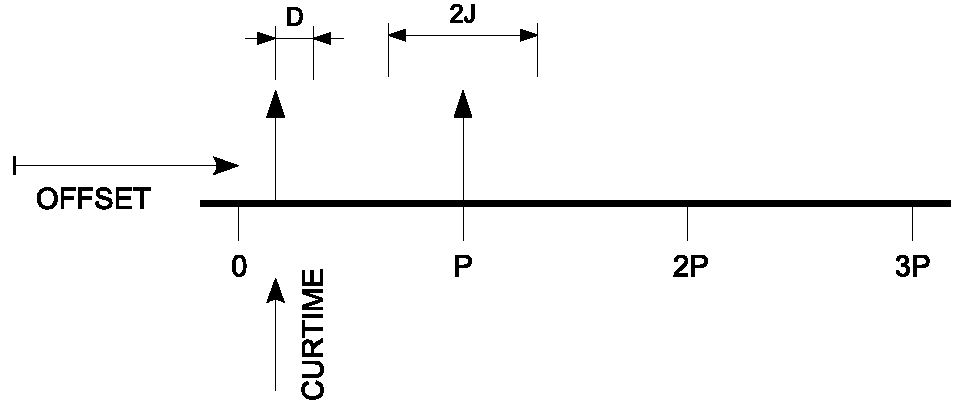
\includegraphics[width=4in]{periodic.eps}
\end{center}
\caption{Example of a periodic event stream with a $(p,j,d,o)$-tuple  $(p,j,d,o)$-組の周期的連続事象の例題\label{fig:perioddef}}
\end{figure}

スレッド間の交信は共有オブジェクトを基に行う。
このように共有オブジェクトの統合を確実に行うためには、同期の仕組みが必要である。この仕組みについては第~\ref{chap:sync}章で述べる.

\subsection{Duration文とCycle文}

Duration文は、モデルの特定部分の実行時間として設定するための固定推定値を許す、VDM++ 文である。
Duration文は次の形式をとる

\begin{lstlisting}
duration (@\textit{time}@) @\textit{文}@
\end{lstlisting}

これは、\emph{statement} の実行に \emph{time} 単位時間かかると推定されることを意味する。
この情報はリアルタイム動作の蓄積のために使われる; この蓄積についての詳細、また何の時間と解釈するべきかの方法論は、以下第~\ref{sec:timingintro}章に記述される。これ以外では、Duration文はその\textit{statement}本体の機能的効果を正確に有している。

Cycle文は、それが配置された\texttt{CPU}に関連するモデルの特定部分の、実行に当てる相対時間の推定を許す VDM++ 文である。
Cycle文は次の形式をもつ

\begin{lstlisting}
cycles (@\textit{命令サイクル}@) @\textit{文}@
\end{lstlisting}

これは、どのようなプラットフォーム上でも\emph{statement} の実行に\emph{instruction cycles}かかると推定されることを意味する。
したがって、2倍の処理速度のプロセッサーが選択された場合に時間は半分になる。
この情報はリアルタイム動作の蓄積において仕様される;この蓄積の詳細、またどのような時間と解釈されるべきかの方法論は、以下の第~\ref{sec:timingintro}章に記述される。
これ以外では、Cycle文はその\textit{statement}本体の機能的効果を正確に有している。

\subsection{システムと環境}

\vdmpp\ では分散システムの記述を可能とするため、モデル化されるシステムの多様な部品が、 
異なる\texttt{CPU}とそれらを互いに結ぶ\texttt{BUS}に対し、どのように配置されるかを表現するシステムの概念が導入されている。
キーワード``\keyw{class}''の代わりに``\keyw{system}''が用いられることを除けば、構文的にこのシステムは通常のクラスとまったく同じに記述される。

このシステムの特異な点は、 \texttt{CPU} と \texttt{BUS}という名の特殊な暗黙に定義されたクラスを、使用することができることである。
システムのインスタンスの生成は不可能であるが、\texttt{CPU} と \texttt{BUS} からなるインスタンスが初期化時に生成される。
 \texttt{CPU} と \texttt{BUS} は、システム定義以外の場所で用いることができないことに注意しよう。

\texttt{CPU} と \texttt{BUS} のインスタンスはインスタンス変数として生成されなければならず、その定義には構成子を用いなければならない。
\texttt{CPU} クラスに対する構成子は2つのパラメーターをとる: 1つ目は\texttt{CPU} に対して用いる基本的なスケジュール化方式であり、2つ目は \texttt{CPU} の処理能力を提示するものである (単位時間としてミリ秒を使用する場合はMillion Instructions Per Second またはMIPSというように示される)。 
\texttt{BUS}クラスに対する構成子は3つのパラメーターをとる。
1つ目はバスの種類、2つ目はバスの処理能力(バンド幅)、最後の3つ目は与えられた \texttt{BUS}インスタンスによって結ばれた\texttt{CPU}インスタンスの集合を示す。

\texttt{CPU}に対して、現時点でサポートされている基本的なスケジュール化方式は次の通り:
\begin{description}
\item[\texttt{<FP>}:] 固定優先度
\item[\texttt{<FCFS>}:] 先着順
\end{description} 

\texttt{BUS}に対して、現時点でサポートされている基本的なスケジュール化方式 (ただし初版ではすべてがFCFSで扱われている)は次の通り:
\begin{description}
\item[\texttt{<TDMA>}:] 時間分割多重アクセス
\item[\texttt{<FCFS>}:] 先着順
\item[\texttt{<CSMACD>}:] 衝突検出型搬送波検知多重アクセス
\end{description} 

VDM++ 技術を使い開発されるシステムの記述に用いた法則は、環境に対しても同様に適用してよい。
つまりキーワード ``\keyw{system}'' を全面的に環境に対しても用いることができるということであり、これによりシステムとその環境間の相互作用の記述が的確にできることを意味する。
これがなされない場合は、システム構成を記述する特殊なクラス``\texttt{World}''内に生成された環境インスタンスのそれぞれに対して、仮想プロセッサー(複数の\texttt{CPU})と仮想交信チャネル (1つの \texttt{BUS}) が設定される。、

\subsection{配置}

\texttt{CPU}クラスは \texttt{deploy} と\texttt{setPriority}という名のメンバー操作を含む。
 \texttt{deploy} 操作は1つのパラメータをとるが、これはシステム内で静的インスタンス変数として宣言されたオブジェクトでなければならない。
配置(deploy)操作の意味論としては、このオブジェクト内の全機能はそれが配置された\texttt{CPU} 上で実行されるということである。
\texttt{setPriority} 操作は2つのパラメータをとるが、1つ目は \texttt{CPU}に配置されたパブリックな操作の名称、2つ目は自然数でなければならない。
\texttt{setPriority} 操作の意味論としては、任意の操作に任意の優先度(2つ目のパラメータ)を設定するということである。
これは、任意の \texttt{CPU}で固定優先度スケジュール化が用いられる場合に使用される。


\section{タイミング分析}\label{sec:timingintro}

 \VDMTools\ を使用してタイミング分析を行う目的は、潜在的な実行時ボトルネックの識別を行うことである。
つまり、そのモデルにおけるスケジュール化上の問題やさらには致命的な遅れを招く失敗の原因となり得る、そういった部分を識別することである。
これで特定の \emph{動的構造} の実行可能性を調べることができる。
動的構造とは、たくさんのプロセッサー上でたくさんのプロセスやスレッドに分解される設計のことである。

\begin{figure}
\begin{center}
\begin{picture}(340,330)
\put(130,270){\framebox(80,60){%
  \parbox{2cm}{\raggedright Model Enhanced With Durations}}}

\put(0,180){\framebox(80,60){%
  \parbox{2cm}{\raggedright Task Switching Overhead}}}

\put(130,180){\framebox(80,60){%
  \parbox{2cm}{\raggedright \VDMTools}}}

\put(260,180){\framebox(80,60){%
  \parbox{2cm}{\raggedright Default Duration Information}}}

\put(130,90){\framebox(80,60){%
  \parbox{2cm}{\raggedright Timed Trace Information}}}

\put(130,0){\framebox(80,60){%
  \parbox{2cm}{\raggedright Trace Analysis}}}

\put(170,270){\vector(0,-1){30}}
\put(170,180){\vector(0,-1){30}}
\put(170,90){\vector(0,-1){30}}
\put(80,210){\vector(1,0){50}}
\put(260,210){\vector(-1,0){50}}
\end{picture}
\end{center}
\caption{タイミング分析へのアプローチ}\label{fig:timing}
\end{figure}

実行時のタイミング表明(形式的に表現される望ましいタイミングプロパティ)の検査は、意図されたタイミング分析の目的ではないし、記述された枠組み内で実行可能だというわけでもない。
さらに、タイミング要求に関する正しい動作を \emph{形式的に検証する} という目的でもない。

上記の目的は、対象の実行構造あるいは用いられるリアルタイムカーネル (述べたような用いられるスケジュール化方式)に従うものである。
上記目的をサポートするために、 \vdmtools\ は対象の実行環境をシミュレートすることを目指す。
対象の環境とは、それ自体が1つのシステムと考えられる環境であるのと同様に、異なるプロセッサーに配置され \texttt{BUS}で結ばれたシステムそのものである。
これは、対象プロセッサーのタイミングプロパティを近似するもので、複数のプロセッサーを結ぶ\texttt{BUS}であり、各プロセッサー上のリアルタイムカーネルによって用いられるスケジュール化方式をまねている。

タイミング動作に関しては、 \vdmtools\ が対象プロセッサーの時刻を\emph{シミュレート}する。
実行中はインタープリタが対象プロセッサーの時計に相当する内部変数の保守を行う、つまり、対象プロセッサーの時計がシミュレートされる、ということである。
インタープリタは最終システムで、別々に分散されたプロセッサーに対し意図したとおりのスケジュール化アルゴリズムを採用する。
モデルの実行中は、様々なプロセッサーに対してたくさんの事象が平行して起きる:

\begin{itemize}
\item スレッドのスワップインとアウト;
\item 操作の要求、活性化、および完了;
\item バス上のプロセス間で通信されるメッセージ.
\end{itemize}

このような事象を、 \emph{トレース事象}と呼ぶ。 
実行中すべてのトレース事象(trace events)は記録され、それらが起きたシミュレート時刻と共にタイムスタンプ(時刻印)が記録される。

タイミング情報については4つのソースが実行中に用いられる:

\begin{description}
\item[cycles文とduration文で拡張されたモデル:] duration文やcycle文のスコープに属するVDM++モデル部分を実行するとき、内部時計は、文の完了時点で、与えられた継続時間/命令サイクルにより進められる。
duration文は絶対時間だが、一方、cycle文はそれが実行されるプロセッサーの速度と関連することに注意しよう。
\item[タスク切り替えオーバーヘッド:] 対象とするリアルタイムカーネルに対してのタスク切り替えオーバーヘッドに対応するために、タスク切り替えオーバーヘッドを定義することができる。
\item[既定継続情報:] duration文のスコープに含まれないモデル部分については、伝統的な最悪事態分析を用いる。
しかしながら、基本的アセンブラ命令を実行するのにかかる時間に関して、キャッシュやパイプライン方式というような可能な限りの最適化技術を考慮することなしに、パラメータ化されている。
想定する対象プロセッサーに対して、ユーザーはアセンブリ命令の時間を定義できる。
このアセンブリ命令から対象プロセッサー上の実行時間への写像を、\emph{既定継続情報}と呼ぶ。
\item[\texttt{CPU}と \texttt{BUS}の処理能力:] 分散システムがモデル化された場合は、システムシナリオの解釈で用いられる\texttt{CPU}と \texttt{BUS}の処理能力
\end{description}

アプローチの概観は 図~\ref{fig:timing}で見ることができる。 
\vdmtools\ は上記で並べたタイミング情報の3つのソースを取上げ、モデルの実行時にこの情報を用いる。
実行中はタイムトレースファイルが生成されるが、タイムスタンプされたトレース事象を発生順に並べたものである。
これは簡単なテキストファイルなので、個々に分析することができる。

\section{本書の構造}

応答システム、VDM++ 、タイミング分析への短い導入の後は、本書は第~\ref{chap:process}章で、 \VDMTools を用いたリアルタイムシステムに対する想定される開発プロセスの比較的簡単な記述を始める。
提示された設計が最終的に実装される前に、そのタイミングプロパティにフィードバックを得ることができるように、上記と同様に本書は、分析および設計フェーズにおける様々なアクティビティに焦点をあてる。
設計過程でのこの一般的な提示の後に、このプロセスに従った実質的な開発例題が第~\ref{chap:example}章で示される。
第~\ref{chap:process} 章では後述の第~\ref{chap:example}章の相当箇所への参照を行っている。
第~\ref{chap:example}章で開発プロセスを描くために用いる例題は、ミサイル防御対策システムである。

その後連続する章では、どのように応答システムの様々な様相がリアルタイムシステムに対する \VDMTools\ 技術を用いてモデル化されるかについて、更に多くの参照を行う。
第~\ref{chap:sync}章では、VDM++で同期をどのように確実化するか説明する。
第~\ref{chap:period}章では、周期的システムや事象のモデル化が説明される。
第~\ref{chap:schedule} 章では、 \VDMTools\ 技術に支えられる様々な種類のスケジュール化方式が表される。
最後に第~\ref{chap:timetrace} 章で、タイミング結果の調整を含む \VDMTools\ を用いてどのような種類の実行後トレース分析が実行され得るかを描く。
第~\ref{chap:example}章では、参照章のいくつかに対する前方参照を多く行う。
したがって、こういった種類の材料にあまりなじみのない読者は、このような参照があるときには参照説明に飛んでみることが有効であろう。

付録としては、用語解説 (Appendix~\ref{app:glossary})、リアルタイムシステムに役立つ設計パターンを少し(Appendix~\ref{app:patterns})、そして最後にすべての例題の列挙 (Appendix~\ref{app:listing})を行っている。

\chapter{リアルタイムシステムのための開発プロセス}\label{chap:process}

この章では、リアルタイムシステムのために提示される開発プロセスの概観を与える。
第~\ref{chap:intro}章で述べた通りここで示す開発プロセスでは、システム分析および設計フェーズのアクティビティに焦点がおかれている。

\begin{figure}
\begin{center}
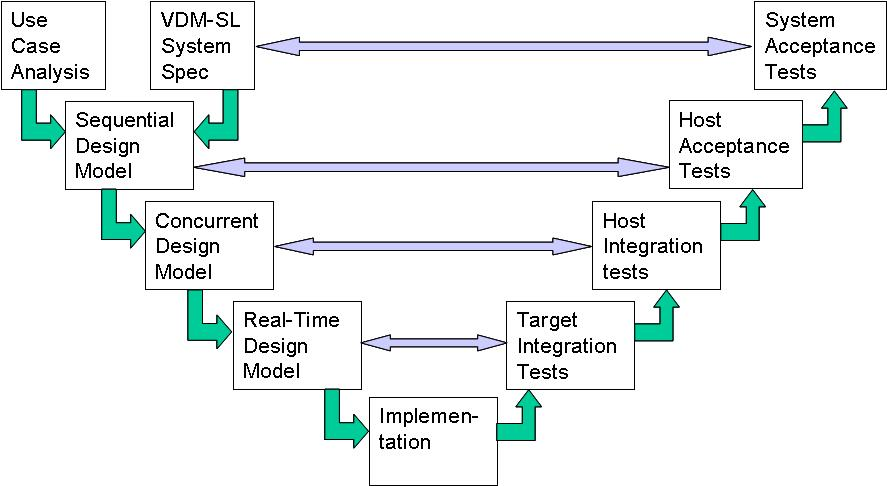
\includegraphics[width=\textwidth]{lifecycle}
\end{center}
%\begin{picture}(350,330)
%\put(0,270){\framebox(80,60){\parbox{2cm}{Sequential Model}}}
%\put(90,180){\framebox(80,60){\parbox{2cm}{Concurrent Model}}}
%\put(180,90){\framebox(80,60){\parbox{2cm}{Concurrent Real-Time Model}}}
%\put(270,0){\framebox(80,60){\parbox{2cm}{Implementation}}}

%\put(40,270){\line(0,-1){60}}
%\put(40,210){\vector(1,0){50}}

%\put(130,180){\line(0,-1){60}}
%\put(130,120){\vector(1,0){50}}

%\put(220,150){\line(0,1){60}}
%\put(220,210){\vector(-1,0){50}}

%\put(220,90){\line(0,-1){60}}
%\put(220,30){\vector(1,0){50}}


%\end{picture}
\caption{開発プロセスの概観}\label{fig:processoverview}
\end{figure}

図~\ref{fig:processoverview} では、この章で言及する様々なフェーズの概観が示されている。
これは伝統的な V-life サイクルであり、 (フェーズ間で繰り返しとフィードバックを行うことで)現実におきていることを近似するものとして多くの産業組織で用いられている。
フェーズのこの構築化は、伝統的なウォーターフォールプロセスと共に用いたり、またBoehmのスパイラルモデル\cite{Sommerville82, Boehm88}を使った各繰り返しに対して用いてもよい。
主な違いとしては、スパイラルプロセスモデルでは最もリスクの高い所産物が最初に分析対象となるということで、つまり以下に述べるプロセスにおいては、最も高いリスクを軽減するために必要とされる分析には何ら影響を与えない部分から抽象化を行う、ということになる。
図中の緑色の矢印は情報の(そしてこの場合は VDM モデルの)基本的流れを示し、一方で紫色の (垂直の) ラインは開発フェーズで (モデルを用いて)行われた検査は相当する受け入れ検査レベルで再生される可能性があることを示す。

開発プロセスは通常、開発するべきシステムの設計から独立した仕様をつくるために、非形式的要求を分析しそれらを捕らえることからはじめる。
この記述に基づいて、システムを静的構造に構築し、システムの逐次 VDM++ 設計モデルを生成する必要がある。
このモデルはその後拡張され、並列VDM++設計モデルとなるだろう。
並列設計モデルは後は自身で、リアルタイムな情報を取り入れることで拡張される。
この段階で、並列設計モデルを再び取り上げることが必要であることが分かる、というのも先の段階でなされた設計決定では、リアルタイム情報がモデルに追加された時点で実行不可能と判明するかもしれないのである (たとえば、モデルはその最終期限に間に合わないかもしれない)。 
並列分散リアルタイムVDM++設計モデルからは、実装が開発される可能性がある。  
最終的な実装の (また様々な設計指向モデルの)検査を行うことが、最も抽象的なモデルを検査の助言者として用いることができることであるのかもしれない。
ここで第~\ref{sec:tests}章の様々な検査フェーズにもどる。

リアルタイムシステムモデルを開発する場合は一般的に、システムをそれが実行され相互に影響している環境から切り離すことは困難である。
したがって、環境すべての関連部分もまたモデル化されることはしばしば起きる。

\section{要求捕捉}

システム開発プロセスの第一フェーズは、新しいシステムの要求を捕捉することである。このフェーズはまたそれぞれの企業標準にしたがい、システム分析フェーズあるいは仕様フェーズとも呼ばれる。
この段階はUML かあるいは VDM-SLを用いることで実施されることが推奨される。
両アプローチにとって、開始点は非形式の要求事項であり、終点はシステム要求の1仕様となるが、図~\ref{fig:inputoutput}で示されるように、設計項目からは独立している。
モデル駆動型アーキテクチャー(MDA) \cite{MDA} の専門用語においては、プラットフォーム独立モデル (PIM)と呼ばれる。

\begin{figure}
\begin{center}
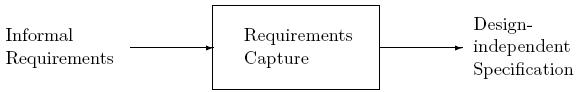
\includegraphics[width=0.8\textwidth]{reqcapture}
\end{center}
\caption{要求捕捉のための入出力関係の概観}\label{fig:inputoutput}
\end{figure}

\begin{figure}
\begin{center}
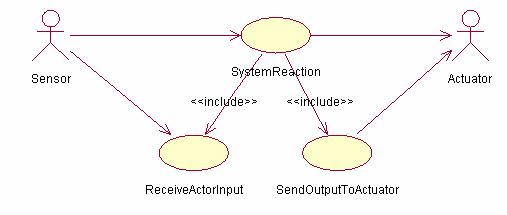
\includegraphics[width=0.8\textwidth]{generalusecase}
\end{center}
\caption{組込みシステム向け汎用ユースケース}\label{fig:usecase}
\end{figure}

両アプローチを続けて説明する。
第~\ref{subsec:capuse}章では標準となった UML \cite{UML20} アプローチを説明し、ここでは use-cases が生成されてクライアントやユーザーと論じられている。
このアプローチはそのミサイル防御対策システムと共に、第~\ref{sec:usecase}章で図つきで描かれている。

もう1つの方法として、変化の少ない VDM-SL モデルと、それに接続されたグラフィカルユーザーインターフェイス(GUI) が、この動画モデルとの相互作用をユーザーやクライアントに許すために生成される可能性もある( \cite{CashPoint}で述べられているのと同様な方法で)。
このアプローチは第~\ref{subsec:VDMSL}章に、第~\ref{sec:VDMSL}章の対策例題と共に、述べられている。

\subsection{UML ユースケースを用いた要求事項の捕捉}\label{subsec:capuse}

この章では、UML ユースケース図 \cite{UML20}を用いて、どのように要求を捕捉できるかを説明している。
ここではRational Roseツール \cite{Rose&00} の使用を仮定するが、他の UML ツールも同様な機能はもっている (今のところ \VDMTools\ 結合を除いては)。

要求分析の例は~\ref{sec:VDMSL}節で説明する。

\subsubsection{アクターとユースケースを見つける}

\begin{itemize}
\item システムの境界とそれらの主要な機能を識別する。
\item システムのアクターを識別する。アクターは設備やユーザーやシステム環境かもしれない。
\item ユースケースを識別する。
\item 各アクターの役割と各ユースケースの目標(ゴール)、をまとめる。
\item アクターとユースケースを調整して関連パッケージにまとめ入れる。
\item ユースケース図(図~\ref{fig:usecase} にこの例題がある)を用いてユースケースを記述する。
\item 状態遷移図を用いてシステムの状態を記述する。
\end{itemize}

\subsubsection{ユースケースモデルを構成する}

\begin{itemize}
\item ユースケース間に関係{\tt <<}includes{\tt >>}を定義する
(例えば \ 図~\ref{fig:usecase}).
\item ユースケース間に関係{\tt <<}extend{\tt >>} を定義する。
\item ユースケース間に汎化関係を定義する。
\item アクター間で汎化関係を定義する。
\end{itemize}

これらのステレオタイプは UML 2.0 標準 \cite{UML20}において定義されている。

\begin{figure}
\begin{center}
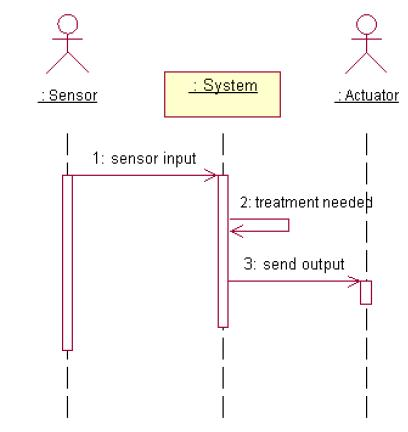
\includegraphics[width=0.5\textwidth]{generalseqdia2}
\end{center}
\caption{組込みシステムのための一般的シーケンス図}\label{fig:seqdiag}
\end{figure}

\begin{figure}
\begin{center}
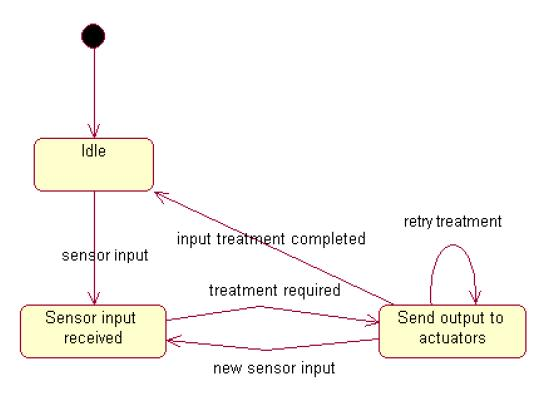
\includegraphics[width=0.8\textwidth]{generalstatedia}
\end{center}
\caption{組込みシステムのための一般的アクティビティ図}\label{fig:activitydiag}
\end{figure}


\subsubsection{詳細にユースケースの仕様を定める}

各ユースケースに対して

\begin{itemize}
\item アクターとシステムの間の相互作用を詳細に記述する。
\item アクターとシステムの間の相互作用を構造化する。
注意したいこととしては、アクションの通常シーケンスと異常時シーケンス(たとえば\ 例外ケース、分解ケース、失敗ケース 他)は区別するべきである 。
\item ユースケースは場合により、既に定義されたユーザーインターフェイスと結び付いているかもしれない。
人間対コンピュータのインターフェイスに特別に関心を払って、こういった面からの開発がなされるべだというわけではないが、ユースケースの便宜的な記述を用いるこのインターフェイス表現は、大いに役に立つ。
\item 役立つならば、ユースケースの全出口シナリオを記述することもできる。ユースケースと結び付いたシナリオとの違いは、シナリオはユースケースの1インスタンスであるということ。
\item 各ユースケースまたはシナリオを描く:
\begin{description}
\item[シーケスンス図を用いる:] この段階で問題あるシステムはクラスに分散されていないため、このようなシーケンス図は単にアクターとシステムの間のコントロールフローを表す。
UML2.0版 では、制御原則 \cite{UML20}の代替フローの情報も含む可能性がある。
典型的なダイアグラムとしては、A4/レター紙上に収まるべきであろう。
この例題は 図~\ref{fig:seqdiag}で見ることができる。
\item[アクティビティ図を用いる] 必要な場合 (これまたはマルチアクティビティ図で)。 この例題は図~\ref{fig:activitydiag}に示されている。
\item[状態図を用いる] ユースケースが複雑となりこの方が適切と判断される場合。
\end{description}
\end{itemize}

\subsection{VDM-SLを用いた要求事項の捕捉}\label{subsec:captureVDM}
\label{subsec:VDMSL}

前記の第~\ref{subsec:capuse}章で述べたユースケースアプローチの代替として、VDM-SLを用いて設計から独立した方法で非公式な要求を補足することが可能である。
最初のインスタンスでは、これが \cite{Fitzgerald&98b,Fitzgerald&05}の第2章に続く。
この段階で、状態変数として含めた時間をモデルの一部に導入することが可能である。
この方法で、機能、タイミング、時間依存機能といった要求が1つのモデル内で捕捉できる。

リアルタイムシステムをモデル化するために用いる一般的な戦略は、そのシステムを1つのトップレベル操作としてモデル化することであり、ここでの入力はシステムに入りモデル化される事象のシーケンスとして考える。
したがってトップレベル操作からの出力が、システムから送り出される事象となる。
時間が本質的なものであれば、すべての入力と出力の事象はその事象が出現した時間でタグ付けされなければならない(つまり\ 事象レコード値の追加項目として)。
こういったVDM-SL モデルでは、この方法で時間が明白にモデル化される。

VDM-SLモデルのトップレベル関数の一般的構造は、次のようなになるだろう(ここではトップレベルで閉鎖ループに伴う複雑な問題は考慮していない):

\begin{lstlisting}
operations

  PerformSystemReaction: seq of SensorInput ==> 
                         seq of ActuatorCommand
  PerformSystemReaction(inputseq) ==
   if inputseq = []
   then []
   else SensorTreatment(hd inputseq) ^ 
        PerformSystemReaction(tl inputseq)
\end{lstlisting}

 \texttt{SensorInput} 型および \texttt{ActuatorCommand} 型は、時間を属性として明示的に含めることができるか、あるいは時間が暗黙的に表現されるように入力間の固定時間間隔がモデル化できる。
センサー入力の処理にかかる時間が次のセンサー入力が到着する時間よりも長くなる場合には、現行の処理に中断がかかる。
その場合、上記で用いた \texttt{SensorTreatment} や\texttt{PerformSystemReaction}関数による機能記述はもっと複雑である。
このようなVDM-SL モデルの完全な例題を第~\ref{sec:VDMSL}章で与える。
当然のことながらこのアプローチを用いて、システムの応答に依存した環境動作を適切に考慮することのできない場所で、フィードバックが繰り返される。
もしセンサー入力のシーケンスがシステム出力シーケンスの順に一致しないとしたら。
それは単純に与えられた入力シーケンスは現実と一致しないことを意味する。
にもかかわらずこのような高レベルの実行モデルは、現実の最終的に装備されるセンサー類に対して助言を与えるものとなることで価値があるだろう。

適切なフィードバックの繰り返しに適応するために、新しくセンサー入力の検知はされなくとも、発行されるアクチュエータ命令と共に単純に蓄積パラメータを導入する必要がある。
蓄積パラメータは、新しいセンサー入力が到着したときにそれに応じて操作を行うことができる。
このアプローチは実際に、第~\ref{sec:VDMSL}章で続けられる。

 VDM-SLモデルをアニメート化し、ユーザーや内部の専門家やクライアントがどのように要求が捕捉されたかがわかる GUI の構築が可能であることには注目したい。
このアニメート化の技術は、入出力関係の点検が可能な場所で、多くのシナリオの視覚化を可能にする。

\subsection{要求捕捉の妥当性検査}

伝統的なライフサイクルでは、テスト計画だけが、システム開発の早い段階 \cite{Sommerville82}で作成される。
ここで述べた開発プロセスの利点の一つは、系統的なテストを行うことを可能とし、ライフサイクルのごく初期の段階で、このようなテスト計画に対するフィードバックを得ることができることである。
変化の少ない VDM-SL アプローチが要求の捕捉に用いられるのであれば、クライアントやユーザーとの対話のために用いたGUIを再利用すべきであり、モデルはクライアントとユーザーの満足のためにアニメート化されるべきである。
完成したシステムの最終的な受入テストではいわゆる概念プロトタイプの証明として、抽象的なVDM-SL モデルの実行から最終的に実装されたシステムの実行までとスクリプトを変化させることで、回帰テスト環境を可能な限り再利用するべきである。

\subsection{完了の基準}

このステージは次の場合に完了する:

\begin{enumerate}
\item 構造的に重要なユースケースが完成して、例えばインスペクションにより、手作業による妥当性検査が行われた、
\item 抽象的VDM-SL モデルが完成し、妥当性検査が行われた。
\end{enumerate}

\section{逐次設計モデル}

逐次設計モデルは、計算されるべきデータとそれをどう静的クラスに構成するかの両方を、特定の動的構造を指定せず記述しなければならない。

逐次モデルを作成する第一段階は、静的な構造を決定することである。
静的な構造は、システム動作をクラス/オブジェクトへ当てはめる準備となる。
クラス構造を導く古典本は既にたくさん存在するので\cite{Rumbaugh&91,Meyer88, Douglass99}、本書ではその論議は含めない。
本書では、どのようにクラスを識別することができるかのガイドラインのみを示し、またシステムで同定されたクラスのそれぞれに対してVDM++ の骨組み(skelton)を生成する際にどの程度まで VDM-SLモデルが再利用できるのかを論じる。

静的な構造の開発を行うことに対するアプローチは、UMLアプローチかVDM-SLアプローチのどちらが要求捕捉に用いられるかに依存する。
これらはしたがって以下で別々に扱う。
どちらの要求捕捉アプローチが用いられたとしても、現在の工程の成果物は常に VDM++クラスの骨組みになるであろう。

\subsection{要求捕捉に UML が用いられる場合}\label{subsec:UMLreq}

要求捕捉のために UMLが用いられた場合、ユースケースがクラスの数を同定するために分析され、これらのクラスから VDM++ クラスの骨組みが生成される。

\subsubsection{クラスを同定する}

このアクティビティは概念を識別することから成り、もっと一般的に言えば、要求捕捉プロセスの結果である仕様からの抽象化で構成される。
また、これらのクラス間では関連が定義されるべきである。
この件については完全な書物があるので、ここでは文献\cite{Kruchten00}から専門用語を引いて短い導入を行うにとどめる。
この段階で、特定のクラスに詳細を加えることよりもクラスを識別することがより重要である。
システム自体に対するクラスと共に、環境からのフィードバック捕捉を可能とする環境所産に対するクラスがあるべきである。
しかしユースケースによって識別される依存関係を基に、いくつかの属性との関係を定義することは可能かもしれない。
これらのクラスから、最初のクラス図が生成される可能性がある。

\begin{figure}
\begin{center}
\begin{tabular}{|l|l|l|l|l|}\hline
         & Actor & {\tt <<}Entity Class{\tt >>} & {\tt <<}Boundary Class{\tt >>} &
           {\tt <<}Control Class{\tt >>} \\ \hline
Actor                        &   N/A  & No & Yes & No \\ \hline
{\tt <<}Entity Class{\tt >>} &  No    &No\footnotemark & No & Yes \\ \hline
{\tt <<}Boundary Class{\tt >>}& Yes   & No & No  & Yes \\ \hline
{\tt <<}Control Class{\tt >>} & No    &Yes & Yes & Yes \\ \hline
\end{tabular}
\end{center}
\caption{クラス間の結合に対する提言\label{tab:assoc}}
\end{figure}
\footnotetext{2つのクラス間に集約単位や構図が存在しない場合。}

各クラスに対しては以下のステレオタイプが用いられるべきである:
\begin{description}
\item[{\tt <<}Entity Class{\tt >>}] このクラスが永続的データを含むことを示す。
\item[{\tt <<}Control Class{\tt >>}] システム中のアクティビティをこのクラスが制御、順序付け、調整することを示す。
\item[{\tt <<}Boundary Class{\tt >>}] このクラスがアクター (システム環境の一部)に対するインターフェイスであることを示す。
\end{description}

クラス間の関連の使用には、多くの提言が適用される。
これらは Table~\ref{tab:assoc} で見つけることができて、``No''は結合すべきでないこと``Yes''は結合され得ることを示している。

\subsubsection{VDM++ クラスの骨組み生成}\label{subsub:skeleton}

クラス定義が終了した場合、次の段階はモデルに対する骨組みとなるVDM++ クラスを生成することである。
クラスの骨組みは、 UMLクラス図と  \vdmtools からの Rose-VDM++ リンクを使用して、自動的に生成される。
これは自動的にRose リポジトリにある各クラスに対し、1つのMicrosoft Word RTF形式ファイルを生成する。
こういったファイルはそれぞれ、そのVDM++ クラスの骨組みを含む。
生成後は、Microsoft Word ファイル中のVDM++モデルと、Rational Rose モデルを相互に調整可能である。Rose-VDM++ リンクは、互いのモデルの変更をマージ(併合)することができる。

\subsection{要求捕捉に VDM-SL が用いられる場合}

形式化されていない(インフォーマルな)要求がVDM-SLで厳密に補足されている場合、VDM-SL 操作のほとんどは、構造や設計上の決定を考慮したVDM++のクラス内で、概念的に再利用可能であることが多い。 (例題 \cite{CashPoint}を参照)。
しかしリアルタイムシステムに対しては、VDM-SL モデルの性質から伝統的なシステム構造で必要とされる設計とはかなり異なるものとなるはずで、この種のシステムの再利用はあまり期待すべきではない。
それでも、このようなシステムの要求捕捉にVDM-SLを使うことは、依然として価値があるだろう。

VDM-SL モデルで形式的な機能要求が定義されたら、それらの要求を静的構造へマップしておくべきである。
骨組み VDM++ クラスは VDM-SLモデルから合成されるべき、ということである。
これは自動的なプロセスではない上に、最も都合よくシステムを分割し構成要素やクラスにする方法についてのガイドラインにおいては、独創的であることとか他のものより優れていることとかを要求しているものでもない。
以下のガイドラインがこの合成において用いられるべきである:

\begin{itemize}
\item VDM-SL モデルのレコード型が、一般的に静的構造におけるクラスとなる。
\item 機能的に独立したアクティビティは、一般的に静的構造において別々のクラスにカプセル化される。
\end{itemize}

複数のクラスやクラス間関係に分割するため、準拠すべきガイドラインがあるとすれば、それは対象システムとその環境の両方をモデル化するものである。
一般的には各々のセンサーやアクチュエータは自身のクラスをもつ。
配置の見通しとして、このようなクラスのインスタンスは一般的にそれら自身の \texttt{CPU}に割当てられる。
これらはユースケース図からアクターと仮定される。
伝統的には、環境と対象システムを表現するクラスの間でのすべての相互作用を調整するような、 \texttt{World} クラスをもつことがよいとされてきた。
このクラスは後に、異なるオブジェクト間に適切な結合を設定し、相互作用のテストに用いられることが可能である。

こういったクラス骨組み合成の例題が第~\ref{sec:skeleton}章に与えられている。

\subsection{VDM++ におけるクラス記述}

クラスの骨組みは徐々に完全な記述へと展開されるのがよい。
このことは、前段階で参照したそれらの操作に対して操作本体を完成することや、いくらかの関数や操作を追加することを含める。

ここで、考え得る型とインスタンス変数の不変条件を特定し、記述すべきである。
事前条件をすべての操作とすべてではない関数に対して指定するべきであり、また事後条件をそれが意味を持つ場所すべてに指定するべきである (つまり\ where 関数や操作本体の再表示を招くことのない場所、があるとすればである)。

VDM++ における完成されたクラス記述の例題は、第~\ref{sec:sequential}章に与えられている。

\subsection{環境のモデル化}

応答リアルタイムシステムの動作のモデル化は、実行環境の参照なしではしばしば困難となる。
この環境を表すクラス(または/あるいは並列モデルにおけるスレッド) を生成することがしばしば好都合となる。
これらクラスは後に、テストデータをもつモデルとして用いられる可能性もある。

\subsection{一般的な設計構造}\label{sec:typicalclassdiag}

\begin{figure}
\begin{center}
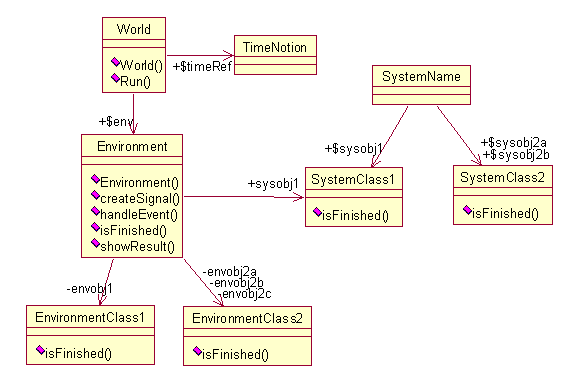
\includegraphics[width=0.8\textwidth]{generalclassdiag}
\end{center}
\caption{組込みシステムのための汎用クラス図}\label{fig:classdiag}
\end{figure}

図~\ref{fig:classdiag} では、本書のガイドラインで応答組込みシステムに対して推奨する一般的静的クラス構造を描く。
\texttt{Environment} に対し責任をもつクラスと、 \texttt{SystemName}という名のシステムの内の要素構成に責任をもつクラスを、常に持つことを推奨する。
また、\texttt{World}という名のクラスを常に持つことも推奨するが、これは環境およびシナリオ実行を可能にするシステム構成要素の両方の設定に責任のある、構成子を含むものである。

シナリオは通常は、 \texttt{Run}という名の操作で起動される。
このように、一般的には \texttt{new World().Run()}というような呼び出しが行えて、シナリオの詳細はパラメーターで与えられるかファイルに保存され標準 \texttt{IO} クラスで読み込まれるかとなる。
応答システムは環境からの刺激に対して応答するため、 \texttt{IO} は一般的に \texttt{Environment} クラスまたは環境の一部を表す他のクラス(図~\ref{fig:classdiag}内の\texttt{EnvironmentClass1} と\texttt{EnvironmentClass2} )のいずれか1つの内部で使用される。

構成子に加え、 \texttt{Environment} にはシステムに対して入力を準備する操作とシステムからフィードバックを受ける操作(handleEvent)を含むことが推奨される。
さらには、シナリオ中で活動的役割を演じるすべてのクラスに対して、 \texttt{isFinished}という名の操作 (この操作は局所的に処理が終了したときに指示される)を提供することも推奨される。
この操作は環境とシステム両方のクラスへのリンクを持つ。
第~\ref{chap:example} 章で示される例題で明らかになるが、逐次モデル中の\texttt{isFinished} のシグネチャは、一般的に論理値の結果を返すが、並列分散モデルでは変化するであろう。
 \texttt{Environment} クラスに対して、
 与えられたシナリオ(\texttt{showResult})の実行結果を見せることのできる、ある種の操作を提供することも必要である。

 \texttt{World}および全体的システムクラスである \texttt{SystemName} に対して、オブジェクト参照のたらいまわしなしにそれらのモデルを通した利用を容易にするためには、静的なパブリックインスタンスの利用が推奨される。
その応答システムにとって時間が重要な場合(通常はそうであるが)、何らかの時間の概念が含まれる。
逐次モデルにおいては基本的な \texttt{Timer} クラスを用いることを推奨するが、並列モデルにおいては時間と同期についてより強い概念を推奨し、第~\ref{sec:designconcur}章で示す。

最後に、制御フローを \texttt{Environment}からはずすことが推奨したい。
逐次レベルでは一般的にこれは繰り返しを用いて行い、システムの終了を行う (様々な \texttt{isFinished} 操作を用いて)。
繰り返しの中で、 \texttt{Step} 操作は時間を刻むためにまたシステムの様々な構成要素に制御を回すために用いられる。

\subsection{モデルの妥当性検査}

可能なら常時、モデルは妥当性検査のために実行されるべきである。
要求捕捉過程でユースケースアプローチが用いられた場合は、識別される全ユースケースでモデルの実行に対応することを保証したい。

すべてのモデルが実行可能ではないとしても、一部がそうであるならば当然これらは上記の方法で妥当性検査されるべきであることを注意したい。

上記のモデル妥当性検査のためのアニメート化の技術に加えて、より系統だった伝統的検査手法もまたモデルの妥当性検査に用いられるべきである。
従って、テストケースを回帰方式でこの工程に使うことができ、その後の工程で再利用できるように、テストケースを定義し自動テストスクリプトも作成するべきである。
\cite{Fitzgerald&05} (chapter~9) で示すVDMUnit テスト・フレームワークを効果的に利用できる可能性がある。

\subsection{完了の基準}

この段階は次の場合に完了する:

\begin{enumerate}
\item  VDM++ モデルの構文と型が正しい;
\item  UML クラス図と VDM++ モデルが同期している;
\item  モデルは既に妥当性検査されている;
\item モデルの実行可能部分に対して XX\%\ テストカバレジ(カバーされない部分は正当であることを示すべきである).
\end{enumerate}

ここで ``XX'' は、各個別の企業や機関で用いられている標準により決定されるべき数字である。

\section{並列 VDM++ 設計モデル}\label{sec:concur}
並列の VDM++ 設計モデルを開発する場合の目標は、特有の動的構造に向けての第一歩を踏み出すことであり、リアルタイム動作の最初のインスタンスへの心配は無用である。
このようなモデルの例題は第~\ref{sec:concurmod}章に与えられている。

\subsection{スレッドの識別}

並列モデルの開発における最初の段階は、どの計算が各々独立に実行可能か識別することである。
これらの計算は後に、独立スレッドに分離される可能性がある。
このような分離は、ハードウェア的制限や事前に定義済みの構造要求によりしばしば強いられることとなる。
可能な限り多くの独立スレッドを識別することが無駄ではない一方、一般的にシステム内のスレッド数は最小化される。
なぜなら(また一般的には) スレッドはモデルの複雑さを増しモデルの妥当性検査をより一層難しくするからである。

\subsection{交信}

スレッドの識別後、どのスレッドが互いに交信しているか、またどのような値が渡されているか、が決定されなければならない。
したがってスレッド間のオブジェクト共有は記述されるべきである。
共有オブジェクトを表すクラスに対しては、適切な同期の指定が求められる。

\subsection{同期ポイント}

オブジェクト共有の同期に加え、明白な同期時点の導入が必要となるかもしれない。
つまり個々のスレッドが、もうひとつのスレッドが適当な状態に到達するまでは指定された時点を越えた続行をしないことを保証することである。
このことは様々なスレッド中に正しい順付けを保証し、他にもデータの新規性の保証に、重要となるはずである。

\subsection{モデルの妥当性検査}

モデルは、対象環境にあるプロセッサーの対象リアルタイムカーネルで、使用されるのと同じスケジュール化方式を用いて実行されなければならない。
実行中にモデルがデッドロックを起こすことがないようにすべきである (\VDMTools\ においてこのために行われる形式的分析はまだないため、シナリオはテストケースとして用いられると限定されることに注意したい)。 
さらにモデルは、逐次モデルと機能的には同じ結果と、恐らくそこに現れる値の体系に伴う調整と、それらが出現した時間をもたらすべきである。

\subsection{一般的な設計構造}\label{sec:designconcur}

 図~\ref{fig:classdiag}にある一般的構造が並列モデルに対して推奨される。
逐次モデルからの主な変更は以下の通り:

\begin{itemize}
\item 制御フローは、\texttt{Environment} と共にある代わりにアクティブな部分すべてに分散され、\texttt{Step}操作の本体は一般的にはスレッドに変化する、というように変更される。
\item 異なるスレッド間の同期は、許可述語と排他制御制約を用いて記述される。
\item  \texttt{isFinished} 操作に対するシグニチャは変更され、値は返されない。
そのかわり許可述語としてブール式が一般的に用いられる。
これがこの操作を求めるスレッドを、対象インスタンスが仕事を終えるまで、遮断する方法となる。
\item 単純な \texttt{Timer} クラスを標準の \texttt{TimeStamp} クラスで置き換えることを推奨する。
これは制御フローが複数スレッドに分散されている場合、今実行している複数のステップを簡単に同期させるためのもので、 Appendix~\ref{sec:TimeStamp} にある \texttt{WaitNotify} クラスのサブクラスである。
\end{itemize}

\subsection{完了の基準}

\begin{enumerate}
\item  VDM++ モデルは構文と型が正しい。
\item  UML クラス図と VDM++ モデルは同期している。
\item モデルは妥当性検査がなされている。
\item モデルはデッドロックを起こしていない;
\item モデルの実行可能部分に対して XX\%\ テストカバレジ
(カバーされない部分は正当とみなされるべきである)。
\end{enumerate}

ここで ``XX'' は、各個別の企業や機関で用いられている標準により決定されるべき数字である。

\section{並列実時間分散VDM++設計モデル}

この段階で、モデルにリアルタイム情報が加わる。
加えて、問題のシステムが複数プロセッサー上に分散されることになるならば、それらプロセッサーに対し機能性配置が行われる。
そして第~\ref{sec:timingintro}章でで述べたタイミング分析が行われる。
このような分析の後、提案された動的構造が実際は実行不可能であるという結果に終わるかもしれない。
したがって第~\ref{sec:concur}章に立ち戻り動的構造を見直すか、または \texttt{CPU}あるいはその許容能力に対して機能性配置の見直しが必要となるかもしれない。
並列実時間モデルの例題は第~\ref{sec:realtime}章で与えられる。

\subsection{既定時間情報(CPU命令毎に想定する実行時間情報}

対象プロセッサーが標準のものでない場合 (現在サポートされているプロセッサーは Motorola 68040 のみ)は、必要な対象プロセッサーに対する既定継続情報を含むファイルが定義されるべきである。 
原則的にこれは単純な定義であり、そのプロセッサーのデータに基づいて行われる。
しかしながらキャッシングやパイプライン構造を用いる近年のプロセッサーでは、様々な基本命令に要する時間が文脈に依存するため、正確な推定はさらに難しいことが予想されるため、この枠組みを考慮することが不可能である。

\subsection{Duration文とCycle文}

モデルのリアルタイム動作が知られている部分 (たとえば 再利用されている構成要素) に対し、固定実行時間の正確な評価にDuration文を用いるべきである。
Cycle文は、1つのプロセッサーに対し相対的な実行時間(期待する命令サイクルという形で)の正確な評価に用いるべきである。

環境を効果的にモデル化するモデル部分に対して。
設計中のシステムの VDM++ モデルに必要とされる精密さに依存するが、環境モデルはさらに精巧であるべきである。
環境内の様々なインスタンス各々を、それらの仮想プロセッサー上にもつことがここで可能である。
しかしながら、例えば複数の環境インスタンスが同一のプロセッサー上に配置されるような制約を行うように、環境をモデル化することもまた可能である。

閉鎖ループシステムをモデル化するためには、アクチュエータに命令を送ることとセンサーでその効果を確認することの間に遅延を強いるために、Duration文が用いられるべきである。

\subsection{タスク切り替えオーバーヘッド}

対象のリアルタイムカーネルに対し、タスク切り替えオーバーヘッドを確認しておくべきであろう。
この値はモデルの実行中、 \vdmtools\ のタスク切り替えオーバーヘッドとして用いられるべきものだからである。

\subsection{一般的な設計構造}\label{sec:designvice}

図~\ref{fig:classdiag} の一般的構造は、リアルタイム分散モデルに対しても推奨されるものだ。
並列モデルからの主な変更点は以下の通り:

\begin{itemize}
\item まず \texttt{SystemName}クラスが変更され、機能を分散する対象であるすべての \texttt{CPU}や \texttt{BUS}に対して追加のインスタンス変数が導入されたシステムとなる。
加えてここに構成子が導入され、静的インスタンス変数の \texttt{CPU}への実際の配置が行われる。
加えて、 \texttt{CPU}のいくつかで優先度に基づくスケジュール化が行われている場合、この構成子内で様々な操作の優先度定義が可能である。
\item 選択的に、 \texttt{Environment} クラスからシステムを生成できる。
これを行わない場合は、\texttt{World} クラスに生成された各インスタンスに対して、 \vdmtools\ は単純に仮想 \texttt{CPU} 上のすべての機能を実行する。
環境の機能が互いに依存することが本質的であるような場合、つまり1つのインスタンスが実行中であるときに本来並列様式のもうひとつのインスタンスが実行は不可能な場合、 \texttt{Environment} に対してシステムを生成することがとても価値があるかもしれない。
\item 
異なるスレッド上で実行を単に始めることが必要な多くの操作は、\texttt{async}キーワードを用いて同期をとることとなる。
基本的に、そういった2つのインスタンスがユーザーに知られることなく異なる\texttt{CPU}に配置されているならば、それらは \texttt{BUS} 上で通信し同期の概念は本質的となっていることに注意しよう。
\item 一部のスレッド (一般的には以前より \texttt{Step}機能をもつもの) は周期的スレッドに変わる。
\item 時刻の明示的な概念は (\texttt{TimeStamp} クラスを用いた並列レベルで)取り除かれる。
時刻は暗黙的で、キーワード \texttt{time} を用いて任意の \texttt{CPU}上で現在時刻を参照することが可能である。
\end{itemize}

\subsection{モデルの妥当性検査}

モデルは、以下の2つ基準を満足させる必要があると同時に、多くの様々なシナリオを用いて実行されるべきである:

\begin{enumerate}
\item この段階に対する完了基準により要求されるテストカバレジを達成すること;
\item 要求捕捉の間に識別されたすべてのユースケースをカバーすること(要求の捕捉にはUML が用いられる)。
\end{enumerate}

この実行は、シナリオ中で計算される値の正確さチェックに、またデッドロックが起きていないことのチェックに用いる。
リアルタイム情報の導入はそれ自体がモデルにデッドロックを起こさせる可能性があるが、スケジューラーが時間なしモデルの実行中になされた決定と異なる決定をそれらに対して行うかもしれないからであることに注意したい。

\subsection{タイミング分析}

モデルを実行することで、後で分析が可能なタイムトレースファイルが生成される (これの例は第~\ref{chap:timetrace}章)。 
分析は以下の通りなされるべきである:

\begin{itemize}
\item 周期的スレッドは指定された期限を見過ごさない。
\item すべてのリアルタイム応答要求に対応がなされる (厳しいリアルタイム期限のすべてに対して再利用のシナリオが対応する)。
\end{itemize}

ここで \texttt{showtrace} という名の外部ツールが、これら時限トレースの自動分析で特に役立つ。
自動的に以下が提供される:
\begin{itemize}
\item 複数の \texttt{CPU}と \texttt{BUS}を含む物理構造のグラフィカルな概観。
\item 複数の \texttt{CPU}間でのすべての実行と交信の概観を提示。
\item 複数のインスタンスの詳細な概観と、単一 \texttt{CPU} におけるそれらインスタンス間の実行と交信の詳細な方法、を提示。
\end{itemize}

\subsection{完了の基準}

\begin{enumerate}
\item モデルは構文と型が正しい。
\item UML クラス図と VDM++ モデルは同期している。
\item モデルはスケジュール化可能である。
\item モデルはデッドロックを示さない。
\item モデルはすべての実行されたシナリオに対して機能的に正しい。
\item モデルは物理的構築に対する機能性の配置を含めている。
\item すべての周期的スレッドには、行われるテストに対する物理構成の選択と共に期限が設けられる。
\item 行われるテストに対して、すべてのリアルタイム応答要求を満たす。
\item モデルの実行可能部分に対して XX\%\ テストカバレジ(カバーされない部分は正当とみなされるべきである)。
\end{enumerate}

ここで ``XX'' は、各個別の企業や機関で用いられている標準により決定されるべき数字である。

\section{実装}

実装へのアプローチは、対象の実装言語およびプログラム構造や性能の制約に依存するものである。
C++ が実装言語ならば、動的なメモリー割当が許され、 \VDMTools\ C++ コードジェネレータの使用が可能である。
これはかなりの労力軽減を意味するが、実装がマウスの1クリックで行えるからである。同様に、 Java が実装言語ならば、 \VDMTools\ Java コードジェネレータの使用が可能である。
しかしながらこのような自動化は、厳密なリアルタイムシステムを求める場合は当てにされるべきものではない。

他の環境では実装は手作業で書かれなければならない。
しかし、モデル化の各段階で獲得される情報の量と深さのおかげで、これが極めて簡単な作業になる。
一般的には、 VDM++ モデルをコードに翻訳するための多くの規則は、かなり機械的に適用することが可能である。
%For instance
%\cite{Bousquet00} gives a list of rules that can be applied to translate
%VDM++ models into an Ada 95 implementation.

\section{別のテストフェーズ}\label{sec:tests}

図~\ref{fig:processoverview} で識別されるように、開発途中のシステムにおいて多くの様々なフェーズがあり、様々なレベルでテストが行われる。
便利な開発技術をもってしても、通常は、開発中のシステムが目指す統合テストフェーズ前に間に合わせることができるかどうか正しい妥当性検査を行うことができない。
もしこれらのテストが指定された期限を越える可能性はないことを示そうとするなら、そのために状況を改善するためのシステム再設計と相当する実装に重大なコストが生じる。本書で述べるアプローチでは、システムに潜在するボトルネックをせめて最終実装がなされる前に見つけることを目指す。
目標は、(開発が行われている)ホストコンピュータを放っておいて、恐らく分散している、想定したハードウェアプラットフォームのタイミングに関する振る舞いの情報とともに、並行リアルタイムVDM++設計モデルのタイミングに関する振る舞いをシミュレートすることである。

\begin{figure}
\begin{center}
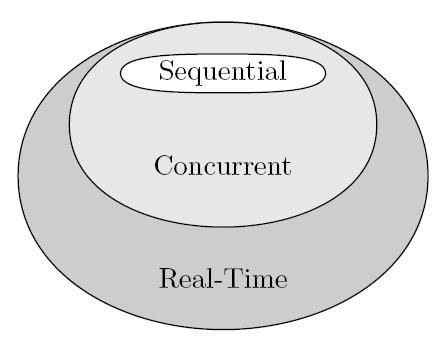
\includegraphics[width=0.5\textwidth]{VDM++levelsofmodels}
\end{center}
\caption{VDM++ モデル間の関係}\label{fig:relationship}
\end{figure}

本書で述べるアプローチでは、様々なテストフェーズで用いられるテストケースは、設計が成され続く最終実装で再利用された段階で、すでに実行されている。
これは開発工程において、特定設計のタイミングプロパティのフィードバックのみがかなり遅れて来る標準的開発手法と比較すると、大きな変更である。
個々のモデル各々はどんなに現実に近づいていくとしても、おおかたの抽象モデルはシステムとその環境をいくらか理想化して見ているもので、より時を経たモデルの方がより詳細までが考慮されている、ということを注意しておこう。

\section{論議}

この章では1つの VDM-SL モデルと3つの VDM++ モデルの進化を述べてきた: 逐次モデル、並列モデル、それに並列実時間モデルである。
それらの間には、どのモデル間にも形式的関係は設定されていないという意味で、形式的な関係はない。
これは、このプロセスで提唱してきた合理的なソフトウェアエンジニアリングアプローチと一致するが、純粋な形式的開発とは相反する。
それでも、このプロセスは次のモデルを得るために各モデルに詳細を加えるという作業を含めるので、図2.6.に見るように、ある意味で各モデルが次のモデルの一部と考えることができる。
つまり、並列モデルは逐次モデルの拡張であり、リアルタイム分散モデルは並列モデルの拡張である。
各モデルは徐々に具体的で複雑なものとなるが、徐々に現実に近づいていくのである。

\chapter{例題の展開}\label{chap:example}

この章では開発工程の例題を提示する。
この開発は第~\ref{chap:process}章からの各手順を経ている。
開発するシステムは実際のリアルタイムシステムの簡易版である。
システムに対する非形式の要求を提示することから始め、その後様々な開発モデルを提示する。

\section{防御対策システム}\label{sec:CMdesc}

 VDM++ でモデル化されるアプリケーションはミサイル防御対策システムのための制御装置である。
これは脅威に関してセンサーからの情報をとり上げ、感知された脅威をそらすことを意図した火炎弾を放つハードウェアに対する命令を送る。
全体的に高レベルの構造が 図~\ref{fig:contextdiag}に見てとれる。

火炎弾は一定の時間間隔で放たれ、発射される火炎弾の数と発射間隔は、ミサイルの脅威と入射角度に依存する
航空機の各所に、異なる火炎弾容器か弾倉が設置され、様々な角度から来る脅威を処理する。
脅威センサーは脅威のIDを制御装置に伝える。
異なる種類のIDとミサイルの角度それぞれに対して、制御装置は、ある角度を処理する特定の火炎弾容器(弾倉)の一定のパターンの火炎弾の連射で、どのように迫り来る脅威を処理するか、対策を立てなければならない。
このパターンは処理すべき火炎弾の数と各発射間の間隔(遅延)を含む。
タスクは、各交信間の指定間隔と既定の発射数を火炎弾発射ハードウェアに伝える
本書の目的に沿うため、2種類の火炎弾しかないと仮定する。

\begin{figure}
\begin{center}

\includegraphics[width=\textwidth]{contextdia}
\end{center}
\caption{防御対策システムのためのコンテキスト図}\label{fig:contextdiag}
\end{figure}

\begin{figure}
\begin{center}
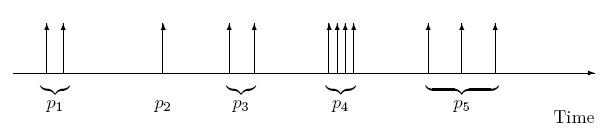
\includegraphics[width=\textwidth]{flareseqs}
\end{center}
\caption{火炎弾シーケンスの例題}\label{fig:firing}
\end{figure}


火炎弾シーケンスの例題は 図~\ref{fig:firing}に示される。
発射命令は垂直矢印で表わされている。
この図には5つのアクションが描かれている。
簡単にするために、システムにはミサイルは3種類だけであると仮定する: A、 B、 C でありこの順に優先度は高くなる。
同様に例題を簡単にするために、物理的な発射は、指定の継続時間に何もされないことを要求する ``空'' の発射を特別に加えて、2種類だけと仮定する。 
この例題の目的のため、示された異なるミサイル型に応答する各火炎弾容器を、図~\ref{fig:missileresp}にある火炎弾シーケンスによって行うための、防御対策システムを仮定する。

このシステムに対して、以下の要求項目が適用される:

\begin{enumerate}
\item もし、与えられた脅威に対する火炎弾容器を用いた火炎弾シーケンスをその火炎弾容器で扱われる角度から計算する間、もう1つの脅威が感知された(同じ角度領域に)場合は、システムはより最新の脅威の優先度をチェックすべきであり、前より大きな脅威である場合には、現在の火炎弾シーケンスの計算を放棄すべきである。
そして新しい火炎弾シーケンスの計算が成されるべきである。
\item もし異なる火炎弾容器で扱われる角度で異なる脅威が感知された場合には、平行して対応する火炎弾シーケンスが実行される。
\item 制御装置は、センサーより脅威情報を受け取った後の250ミリ秒以内に、最初の発射コマンドを送る能力を持つべきである。\label{timereq34}
\item 制御装置は130 ミリ秒以内に火炎弾シーケンスを破棄する能力を持つべきである。
\end{enumerate}

開発されるべきシステムは、編成される物理構造は未定の様々なハードウェア部品 (センサーや火炎弾容器)から成る可能性がある。

\section{要求捕捉のためのUML ユースケース}\label{sec:UMLreq} 
\label{sec:usecase}

防御対策システムに対する要求捕捉のためにユースケースを用いるならば、図~\ref{fig:counteruse}にあるようなユースケース図を提供する。
各長円形(ユースケースのグラフィカル表現)に対して、ユースケースのテキスト記述が必要である。
これは一般的には箇条書きでなされる。
以下の3つの小章で、異なるユースケースのそれぞれに対する記述を示す。

\begin{figure}
\begin{center}
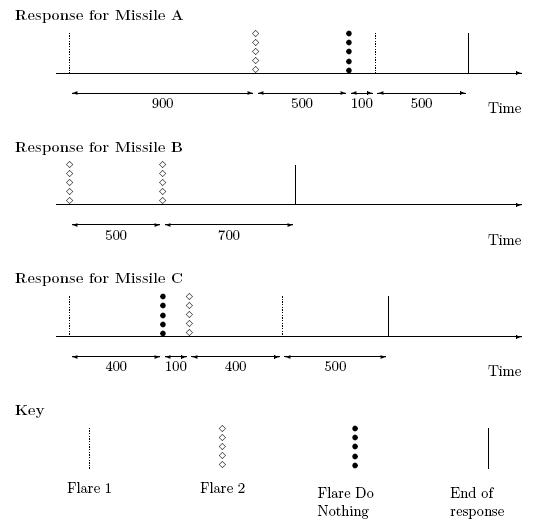
\includegraphics[width=\textwidth]{responses}
\end{center}
\caption{モデル中で用いられるミサイル防御対策例\label{fig:missileresp}}
\end{figure}

\begin{figure}
\begin{center}
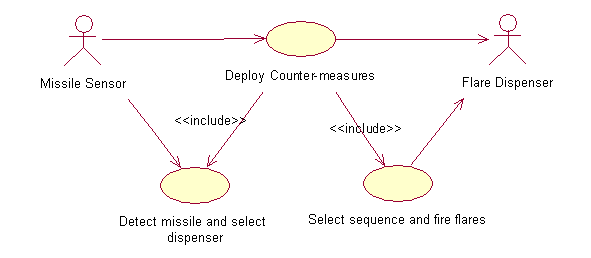
\includegraphics[width=\textwidth]{CMusecases}
\end{center}
\caption{防御対策システムのためのユースケース図\label{fig:counteruse}}
\end{figure}

\subsection{防御対策を展開する}

\begin{description}
\item[Primary Actor(s):] ミサイルセンサーと火炎弾容器
\item[Secondary Actor(s):] なし
\item[Intent:] このユースケースは、与えられた脅威を識別することそれにしたがった発射に、責任がある。
\item[Assumptions:] すべての潜在する脅威が識別される。
\item[Known Limitations:] 複数の脅威が互いに近づき過ぎた場合、システムはそれらすべてをうまく処理することができないかもしれない。
\item[Includes:] ``ミサイル検知と容器選択'' および ``シーケンス選択と発射''
\item[Pre-conditions:] 脅威は到着していてミサイルセンサーに検知されている。
\item[Course of action:] 新しい脅威であるミサイルがミサイルセンサーにより検知されたとき、攻撃の角度に対して適切な火炎弾容器が決定されなければならない。
それから、もう1つの脅威が既にその火炎弾容器によって扱われているかどうかを決定しなければならない。
この場合には、脅威識別の優先度が比較されて、
もし新しい脅威がより高い優先度をもつのであればその火炎弾シーケンスが決定されなければならず、その火炎弾容器は現在行っていることを中止し新しいシーケンスの発射を始めなければならない。
優先度が等しいかより低い場合その脅威は単に無視される。
もし脅威がそれ以前に検知されてない場合、対応する火炎弾シーケンスが決定され、続けてその火炎弾容器を用いて発射される。
これは図~\ref{fig:counterstate}で示された状態図に描かれている。
\item[Post-conditions:] 火炎弾の発射が完了したとき、脅威はそらされ、ミサイル対応策システムによって守られるシステムが、もはや目標となることはないようにすべきである。
\end{description}

\subsection{ミサイルを検知し容器を選択する}

\begin{description}
\item[Primary Actor(s):] ミサイルセンサー
\item[Secondary Actor(s):] なし
\item[Intent:] このユースケースは、特定の脅威の識別と攻撃角度の認識を行い、この測定に基づいてどの火炎弾容器を選択するかについて責任を持つ。
\item[Assumptions:] すべての潜在する脅威が識別される。
\item[Known Limitations:] 複数の脅威が互いに近づき過ぎた場合、システムはそれらすべてをうまく処理することができないかもしれない。
\item[Includes:] なし。
\item[Pre-conditions:] 脅威は到着していてミサイルセンサーに検知されている。
\item[Course of action:] 脅威の識別と攻撃角度を受け取ったときは、いつでも、対応する火炎弾容器を選択し、図~\ref{fig:missileresp}の識別に従って火炎弾列を発射しなければならない。
\item[Post-conditions:] 正しい火炎弾容器と行われるべき火炎弾シーケンスが識別されている。
\end{description}

\subsection{シーケンスの選択と火炎弾発射}

\begin{description}
\item[Primary Actor(s):] 火炎弾容器
\item[Secondary Actor(s):] なし
\item[Intent:] このユースケースは、第~\ref{sec:CMdesc}章に記述したタイミング要求にしたがった火炎弾シーケンスの、実際の発射に責任がある。
\item[Assumptions:] すべての潜在する脅威が認識される。
\item[Known Limitations:] 異なる火炎弾がどのくらい短い間隔で発射できるかについて、恐らく物理的な制限が存在する。
\item[Includes:] なし
\item[Pre-conditions:] 火炎弾シーケンスは識別されている。
\item[Course of action:] 内部時計がスタートし火炎弾シーケンスにより識別された時刻に火炎弾容器による別々の発射がなされた。
\item[Post-conditions:] すべての必要な火炎弾が発射された。
\end{description}

\begin{figure}
\begin{center}
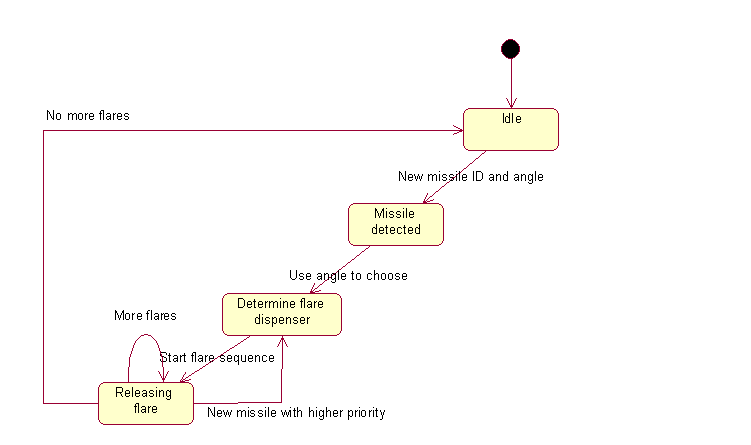
\includegraphics[width=\textwidth]{CMstate}
\end{center}
\caption{防御対策システム展開のための状態図\label{fig:counterstate}}
\end{figure}

\subsection{要約}

上記のユースケース記述から理解できるとおり、防御対策システムの主要機能はユースケースによって識別される。
これはシステムを抽象化して考察する手法で、開発プロセスにおいて後で考慮しなければならない様々な設計事項からは独立したものである。
ユースケースは、他分野の専門家にシステムの重要な機能を把握していることを伝える、最初の方法となり得る。
ユースケース図は、どのようにして様々なユースケースがつじつまが合うのか、特に、より複雑なシステムをモデル化する場合に、概観を得るにふさわしい方法になり得る。
しかしながら、ユースケースのどのような妥当性検査も、手作業的なレビューでしか行うことができない。
上記で述べたような自然言語形式を取り扱うとき、自動化された妥当性検査を実行できる何らの方法もない。

\section{要求捕捉のためのVDM-SL}\label{sec:VDMSLreq}\label{sec:VDMSL}

この章では、防御対策システムに対する要求が VDM-SLを用いた的確な方法で獲得される。 
この意図は、どのような設計事項からも独立な抽象的仕様とすることである。
モデルの開発は第~\ref{subsec:UMLreq}章からの一般的原則にしたがう。 
この最初のモデルでなされる基本的なモデル化決定事項は、最初のミサイルを点検すること、それが唯一の受け取った脅威であったならば適切な応答は何であるべきかを決定すること、である。
現在のミサイル処理を行う前に、1つ以上の更なるミサイルが領域に到着している場合、新しいミサイルの優先度が現在のものより高いときには応答が変更される。

\subsection{型の定義}\label{subsec:generaltypes}

防御対策システムは入力として \texttt{MissileInput}を取り込む。
これは \texttt{MissileType} と\texttt{Angle}のペアの値の連続である。 
\texttt{MissileType}は検知することのできる様々な可能なミサイルを表す定数値である。
この場合には3つの異なるミサイルをもつが、テスト目的のために、何のミサイルも存在していないことを表す特別な値 \texttt{<None>}を共に加える。
簡単にするため\texttt{Angle} は 0 から 360 の数の度数としてモデル化される(2次元座標系に対応し得る一つのモデル).

\begin{lstlisting}
types
  
MissileInputs = seq of MissileInput;

MissileInput = MissileType * Angle;

MissileType = <MissileA> | <MissileB> | <MissileC> | <None>;

Angle = nat
inv num == num <= 360;
\end{lstlisting}

型 \texttt{Output} は、弾倉に対する識別子 (\texttt{MagId})からOutputStepsシーケンスへの写像を表し、ここで \texttt{OutputStep}は行われる火炎弾の型 (\texttt{FlareType}) とその発射の時間(ミリ秒でモデル化されている\texttt{AbsTime} )との対である。

\begin{lstlisting}
Output = map MagId to seq of OutputStep;

OutputStep = FlareType * AbsTime;

AbsTime = nat;
\end{lstlisting}

ここには2種類の火炎弾(\texttt{FlareOne} と \texttt{FlareTwo})しか仮定されていないこと、さらにまた何もしないというアクションはある脅威に対する応答として極めて重要となる可能性があり、そのため火炎弾の一種として考えられるていること、には注意したい。
これらのすべては応答している対象のミサイル型にしたがって追加的にタグ付けされたもので、生成された結果を簡単に妥当性検査するためのものである。

\begin{lstlisting}
FlareType = <FlareOneA> | <FlareTwoA> | <FlareOneB> |
            <FlareTwoB> | <FlareOneC> | <FlareTwoC> |
            <DoNothingA> | <DoNothingB> | <DoNothingC>;
\end{lstlisting}

\texttt{Plan} は出力の構築中に使用される。
これは、発射される火炎弾の型 \texttt{FlareType} と、発射の後に次の発射までの待ち時間の総和である\texttt{Delay}から構成される。

\texttt{Response}はミサイル対応策システムの応答を表す型であり、 \texttt{Plan} 列中の各要素と同じく、\texttt{FlareType} と\texttt{Delay}から構成される。

\begin{lstlisting}
Plan = seq of (FlareType * Delay);

Delay = nat;

Response = FlareType * Delay;
\end{lstlisting}

\subsection{値定義}

異なるミサイルにどのように対処するかに関する情報が\texttt{responseDB} にある(ミサイルから応答シーケンスへの写像で 図~\ref{fig:missileresp}で識別されると同様に\texttt{Plan} に示されている)。

\begin{lstlisting}
values

responseDB : map MissileType to Plan =
 {<MissileA> |-> [mk_(<FlareOneA>,900), mk_(<FlareTwoA>,500),
                  mk_(<DoNothingA>,100), mk_(<FlareOneA>,500)],
  <MissileB> |-> [mk_(<FlareTwoB>,500), mk_(<FlareTwoB>,700)],
  <MissileC> |-> [mk_(<FlareOneC>,400), mk_(<DoNothingC>,100),
                  mk_(<FlareTwoC>,400), mk_(<FlareOneC>,500)]
 };
\end{lstlisting}

ミサイル間の相対的な優先度が\texttt{missilePriority}を用いて表されていて、これは各ミサイルを数字にマップするもので、より大きな数字がより高い優先度を示す。

\begin{lstlisting}
missilePriority : map MissileType to nat
                = {<None>     |-> 0,
                   <MissileA> |-> 1,
                   <MissileB> |-> 2,
                   <MissileC> |-> 3};
\end{lstlisting}

入力の各値は100 ミリ秒間隔で分ける。
ミサイル到着の間のより大きな間隔は、入力中の値\texttt{<None>}で示される。
シンボリック定数 \texttt{stepLength} をこの時間間隔を表すために用いる。

\begin{lstlisting}
stepLength : nat = 100
\end{lstlisting}

\subsection{防御対策機能}

トップレベル関数は \texttt{CounterMeasures}と名付けられている。 
これは入力として\texttt{MissileInputs}を取り入れ \texttt{Output}を返す。 
単純な補助関数 \texttt{CM}の呼出しから構成される。

\begin{lstlisting}
functions

CounterMeasures: MissileInputs -> Output
CounterMeasures(missileInputs) ==
  CM(missileInputs,{|->},{|->},0,{});
\end{lstlisting}

防御対策関数の反復版である \texttt{CM}は4つのパラメーターを取る。
それらは次のように説明できる:

\begin{description}
\item[\texttt{missileInputs}:] このパラメーターはどの火炎弾発射が成されるべきかの分析で、まだ考慮されていないミサイル入力を含める。
このパラメーターについては各再帰呼び出しでこのシーケンスが1つ減じるように再帰が行われる。
\item[\texttt{outputSoFar}:] このパラメーターは、今までのところ考慮されたミサイル入力を与えられて、弾倉識別子から行われる予定の火炎弾シーケンス(そしてそれらの予定発射時間)への写像 を含める。
これは蓄積パラメーターで、最後に最終結果を含むことになる。
\item[\texttt{lastMissile}:] このパラメーターは、弾倉識別子から、今までのところ\texttt{MagId}に関連して出力に影響を与えた最後のミサイルへの写像を含める。
このミサイルの優先度は、次のミサイルの到着に関連し、重要である。
\item[\texttt{curTime}:] このパラメーターはこのミサイルが検知されてきた時間 (\texttt{stepLength}の倍数)を指定する。
\end{description}

防御対策を考慮するためのミサイルが1つも残っていない場合には、\texttt{outputSoFar} が直接用いられる。
そうでない場合は、次に到着するミサイルの優先度が \texttt{lastMissile}と比較されなければならない。
新しく到着するミサイルの優先度が最後のミサイルより高い場合には、出力のための既存の計画を中断し代わりに新しいミサイルに対する応答を組み入れなければならない。
他方で優先度がより低い場合は、最新のミサイルは無視される。
\newpage

\begin{lstlisting}
CM: MissileInputs * Output * map MagId to [MissileType] * 
    nat -> Output
CM( missileInputs, outputSoFar, lastMissile, curTime) ==
  if missileInputs = []
  then outputSoFar
  else let mk_(curMis,angle) = hd missileInputs,
           magid = Angle2MagId(angle)
       in
         if magid not in set dom lastMissile or
            (magid in set dom lastMissile and
             missilePriority(curMis) > 
             missilePriority(lastMissile(magid)))
         then let newOutput = 
                     InterruptPlan(curTime,outputSoFar,
                                   responseDB(curMis),
                                   magid)
              in CM(tl missileInputs, newOutput, 
                    lastMissile ++ {magid |-> curMis},
                    curTime + stepLength)
         else CM(tl missileInputs, outputSoFar, 
                 lastMissile,curTime + stepLength);
\end{lstlisting}

関数 \texttt{InterruptPlan} は、より高い優先度に対する応答を出力に組み入れることができるように、これまでの予期された出力を修正するのに用いられる。
この意味は、\texttt{curTime} より前の出力は変更されることはなく、他方の \texttt{curTime}時点以降の出力は任意の \texttt{Plan}\footnote{\texttt{Output} は絶対時刻に関するものである一方で、 \texttt{Plan} は相対時刻に関するものである。}から採られるということである。
このようにここで転換を行う必要があり; これは\texttt{MakeOutputFromPlan}で実行される。

\begin{lstlisting}
InterruptPlan: nat * Output * Plan * MagId -> Output
InterruptPlan(curTime,expOutput,plan,magid) ==
  {magid |-> (if magid in set dom expOutput
              then LeavePrefixUnchanged(expOutput(magid), 
                                        curTime)
              else []) ^
              MakeOutputFromPlan(curTime, plan)} 
  munion
  ({magid} <-: expOutput);
\end{lstlisting}

\texttt{LeavePrefixUnchanged} は、現時点より前の出力が最新のミサイル到着によって影響を受けることがないことを保証する。

\begin{lstlisting}
LeavePrefixUnchanged: seq of OutputStep * nat -> 
                      seq of OutputStep
LeavePrefixUnchanged(output_l, curTime) ==
  [output_l(i) | i in set inds output_l
               & let mk_(-,t) = output_l(i) in t <= curTime];
\end{lstlisting}

\texttt{MakeOutputFromPlan} は \texttt{curTime} 時点で始まった応答シーケンス(\texttt{response}) を加工し、それを \texttt{Output} 値に変換する。 
これは応答列を出力に変換するが、そこでは最初の火炎弾発射が0という時刻に行われたとする。
この出力は現在時刻で補正され、目的の出力を実現する。

\begin{lstlisting}
MakeOutputFromPlan : nat * seq of Response -> seq of OutputStep
MakeOutputFromPlan(curTime, response) ==
  let output = OutputAtTimeZero(response) in
    [let mk_(flare,t) = output(i)
     in
       mk_(flare,t+curTime)
    | i in set inds output];
\end{lstlisting}

関数 \texttt{OutputAtTimeZero} は1つの応答を取上げ、最初の火炎弾発射はゼロ時刻に行ったという出力に変換する。
その後は、発射と発射の間の遅延は応答により指定された遅延に相当することになる。

\begin{lstlisting}
OutputAtTimeZero : seq of Response -> seq of OutputStep
OutputAtTimeZero(response) ==
  let absTimes = RelativeToAbsoluteTimes(response) in
    let mk_(firstFlare,-) = hd absTimes in
      [mk_(firstFlare,0)] ^
      [ let mk_(-,t) = absTimes(i-1),
            mk_(f,-) = absTimes(i) in
          mk_(f,t) | i in set {2,...,len absTimes}];
\end{lstlisting}

関数 \texttt{RelativeToAbsoluteTimes} は、相対時間の遅延から絶対時間の遅延への変換を実行する。
これは、最初の火炎弾発射の遅延で、応答中の後の火炎弾の発射を、再帰的に相殺する。
\newpage

\begin{lstlisting}
RelativeToAbsoluteTimes : seq of Response -> 
                          seq of (FlareType * Delay)
RelativeToAbsoluteTimes(ts) ==
  if ts = []
  then []
  else let mk_(f,t) = hd ts,
           ns = RelativeToAbsoluteTimes(tl ts) in
         [mk_(f,t)] ^ [ let mk_(nf, nt) = ns(i)
                        in mk_(nf, nt + t)
                      | i in set inds ns];
\end{lstlisting}

\texttt{Angle2MagId} 関数は、ミサイルの入力の角度からそのミサイルに対処する弾倉への変換を行う。
この初期の高レベルのモデルでは、この関数は、単純にそれぞれがテスト目的に90度を処理するハードコードされた4つの異なる弾倉を扱う。

\begin{lstlisting}
Angle2MagId: Angle -> MagId
Angle2MagId(angle) ==
  if angle < 90
  then mk_token("Magazine 1")
  elseif angle < 180
  then mk_token("Magazine 2")
  elseif angle < 270
  then mk_token("Magazine 3")
  else mk_token("Magazine 4");
\end{lstlisting}

\subsection{モデルの妥当性検査}

モデルの機能性が適切であるという信頼を得るために、何らかの形でそれを妥当性検査することが必要である。
このモデルは VDM-SL で作成されているので、幸運なことに\VDMTools のVDM-SL 版を用いてこれを妥当性検査することが可能である。
モデルは、いったん構文および型のチェックがなされると、\texttt{CounterMeasures}という名の main 関数が意図された様式で動作する。
ここでの戦略はいつものようにテストを伴うもので、簡単な値から始めて徐々にもっともっと複雑なシナリオを産みだすことである。
この場合例えば、それぞれ到着するはずのミサイルが1つだけであるとした場合の動作のテストから始めることができるであろう。

Appendix~\ref{app:VDMSLmodel} では、3つの値定義が、もっと複雑なシナリオでテストが繰り返されたことを表わしている。
これら3つは、 \VDMTools のテストカバレジ機能を使って見ることができて、十分にモデルのすべての部分を対象としていることが判明した。
このVDM-SLによる最初のモデルは、様々なタイミング遅延を考えない抽象化を行っているが、それでもシステムの特定のタイミング要求(~\pageref{timereq34}ページ の項目3、4で記載されている)を検査する意味がある。
両タイミング要求はまた、与えられたシナリオと共に妥当性検査される。

\subsection{要約}

第~\ref{sec:VDMSLreq}章では、防御対策システムをかなり抽象化したモデルが提示されている。
第~\ref{subsec:captureVDM}章に述べたような VDM-SLを用いてリアルタイムシステムの仕様を定めるための一般的な法則に、このモデルがどのようにしたがっているのかに注意しよう。
このモデルは、後でシステムをバラバラにして静的構成物(クラス)と動的構造(スレッド)にするために考慮される必要が生じる、どのような設計事項からも完全に独立である。
このモデルの最もよいところは、どのような詳細設計もなく正確に防御対策システム要求の特性を示すことである。

このモデルはたくさんのテストケースでテストされてきた。
時間の重要な部分については、これらのテストケースがシナリオの広範囲をカバーし、モデルが期待された結果を引き渡した、ことを裏付けることに努力が払われてきた。
しかしながらこの努力において、2つの見返りがあった: 第一に、テストケースはシステムの受入れテスト中に再利用可能であること; 第二に、 VDM-SL モデルは後続モデルの開発中にその機能的な動作の比較を行うことで、助言としての使用が可能であること。

この抽象モデルから学べることは、防御対策システムが意図している動作が何かの共通の理解を得ることができて、それが最終実装が完了するときに助言として与えることが可能であるというである。
しかし、これは防御対策システムの理想化版であると心に留めておかなければならないことに、注意したい。

\section{VDM++ クラス骨組み}\label{sec:skeleton}

この章では、第~\ref{subsub:skeleton}章と第~\ref{sec:typicalclassdiag}章で論じられたのと同様に、防御対策システムのさまざまなクラスへの最初の分解がどのように達成できるかの考察がなされる。
システムを構造化することをクラスへと導くのに用いてきた主要なガイドラインは、モデル化において環境を含めることが必要であるということである。
これは、システムのセンサーやアクチュエータをシミュレートするクラスを持たなくてはならないことを意味する。

第~\ref{sec:VDMSLreq}章で表示されている主なアクティビティは、ミサイル検知と火炎弾発射である。
加えて、システムにミサイル到着の警告を与えるハードウェアであるセンサーをシミュレートするクラスをもつことを、期待することになるだろう。
このため4つの候補クラスを挙げ、それぞれを \texttt{MissileDetector}、\texttt{FlareController}、 \texttt{FlareDispenser} 、 \texttt{Sensor}、と名づける。

第~\ref{subsec:captureVDM}章で論じたとおり、 第~\ref{sec:UMLreq}章で提示したユースケースも、第~\ref{sec:VDMSLreq} 章で提示した VDM-SL 仕様も、システムのこの構造化に大いなる助けを提供してはくれない。
これがリアルタイムシステムであるために、 VDM-SL モデルの全部品を再利用することもまた簡単ではない。

\section{逐次 VDM++ 設計モデル}\label{sec:seqVDM}\label{sec:sequential}

逐次モデルは以下のクラスをもつ:

\begin{description}
\item[\texttt{CM}:] これは全体的システムクラスであり (\texttt{SystemName} クラス) すべてのシステム構成要素に対する静的パブリックインスタンスを生成する。 
\item[\texttt{World}:]  main クラスであり、複数のシステムクラスと環境を結びつけシナリオを実行させるのに用いられる。
\item[\texttt{Environment}:] 環境をモデル化するのに用いられる (この場合センサーがシステムに対する入力提供を行う)。
\item[\texttt{Sensor}:] 与えられた角度でミサイル到着を感知するのに用いるハードウェアをモデル化するためのクラス。
\item[\texttt{MissileDetector}:]  \texttt{Sensor} から情報を取り込み、それを \texttt{FlareController}の1つに渡すクラス。
\item[\texttt{FlareController}:] たくさんの火炎弾容器を用いて与えられた検知済みミサイルに向けた火炎弾出力を制御するクラス。
\item[\texttt{FlareDispener}:] ミサイル型に依存する実際の火炎弾を使いこなすクラス。
\item[\texttt{Timer}:] 逐次 VDM++ モデルを通して時間を刻むのに用いられるタイマークラス。
\item[\texttt{IO}:]  VDM++ 標準ライブラリクラス。
\item[\texttt{GLOBAL}:] たくさんのシステムクラスや環境クラスで使用されたたくさんの一般的定義を提供するスーパークラス。
\end{description}

様々なクラス間関係の概観を 図~\ref{fig:classdiagseq}で見ることができる。

\begin{figure}
\begin{center}
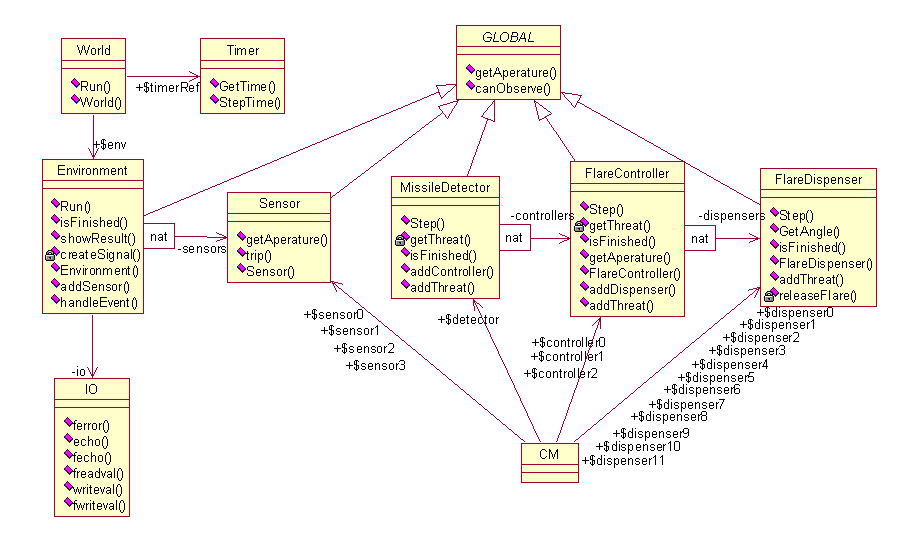
\includegraphics[width=\textwidth]{seqCMclassdiag}
\end{center}
\caption{逐次防御対策モデルのためのクラス図\label{fig:classdiagseq}}
\end{figure}

\subsection{防御対策クラス}

これは、第~\ref{sec:designvice}章の \texttt{SystemName}に相当する \texttt{CM} という名の全体的システムクラスである。
第~\ref{sec:VDMSLreq}章で4つの異なる弾倉 (または火炎弾容器) がそれぞれ90度をカバーしつつ用いられた。
実際にはさまざまな数のセンサーやアクチュエータを用いることが可能である。
原則的には全体的システムに対する耐障害性を増加するために、部分的に重なるセンサーやアクチュエータを重複してもつことも可能である。
本書で記述したVDM++フレームワークを用いて、これがどのように成し得るかを示す設計例を以下に示す。
\begin{itemize}
\item 4つのセンサーが各々90度の角度を対象としている;
\item 1つのミサイル検知機;
\item 3つの火炎弾制御機が120 度の角度をカバーし、それぞれ4つの火炎弾容器を制御する;
\item 12の火炎弾容器が各々30度の角度に対応する。
\end{itemize}

この方法で各々の火炎弾制御装置はそれぞれを制御する4つの火炎弾容器をもつであろう。
以下で明らかになるであろうが、これは少々複雑なシステムであるのだが、センサー、火炎弾制御装置、火炎弾容器の代替構成要素を詳しく調べこれを再構成することを簡単にする様式でモデル化されている。

\texttt{CM} クラスにおいては次のように記述されている:
\newpage

\begin{lstlisting}
class CM
instance variables

public static 
detector : MissileDetector := new MissileDetector();
public static sensor0 : Sensor := new Sensor(0);
public static sensor1 : Sensor := new Sensor(90);
public static sensor2 : Sensor := new Sensor(180);
public static sensor3 : Sensor := new Sensor(270);
public static 
controller0 : FlareController := new FlareController(0);
public static 
controller1 : FlareController := new FlareController(120);
public static 
controller2 : FlareController := new FlareController(240);
public static 
dispenser0 : FlareDispenser := new FlareDispenser(0);
public static 
dispenser1 : FlareDispenser := new FlareDispenser(30);
public static 
dispenser2 : FlareDispenser := new FlareDispenser(60);
public static 
dispenser3 : FlareDispenser := new FlareDispenser(90);
public static 
dispenser4 : FlareDispenser := new FlareDispenser(0);
public static 
dispenser5 : FlareDispenser := new FlareDispenser(30);
public static 
dispenser6 : FlareDispenser := new FlareDispenser(60);
public static 
dispenser7 : FlareDispenser := new FlareDispenser(90);
public static 
dispenser8 : FlareDispenser := new FlareDispenser(0);
public static 
dispenser9 : FlareDispenser := new FlareDispenser(30);
public static 
dispenser10 : FlareDispenser := new FlareDispenser(60);
public static 
dispenser11 : FlareDispenser := new FlareDispenser(90);

end CM
\end{lstlisting}

\subsection{World クラス}

 \texttt{World} クラスは2つの静的パブリックインスタンス変数と2つの操作から構成される。
2つのインスタンス変数は \texttt{env}ironment と \texttt{timerRef} を参照し、environment と systemクラスの両方に用いられる。

\begin{lstlisting}
class World

instance variables
  
public static 
env : [Environment] := nil;
public static timerRef : Timer := new Timer();
\end{lstlisting}

構成子である \texttt{World} はオブジェクトトポロジーを築くため (センサー、環境に対する制御装置と容器、検知機、様々な制御装置をそれぞれに追加する)に用いられる。
原則として \texttt{new Environment} は\texttt{instance variables} のセクションに作成できるはずであるが、これは \vdmtools の初期化において無限再帰を導入することになるのである。

\begin{lstlisting}
operations

public World: () ==> World
World () ==
 (  -- set-up the sensors
    env := new Environment("scenario.txt");
    env.addSensor(CM`sensor0);
    env.addSensor(CM`sensor1);
    env.addSensor(CM`sensor2);
    env.addSensor(CM`sensor3);

    -- add the first controller with four dispensers
    CM`controller0.addDispenser(CM`dispenser0);
    CM`controller0.addDispenser(CM`dispenser1);
    CM`controller0.addDispenser(CM`dispenser2);
    CM`controller0.addDispenser(CM`dispenser3);
    CM`detector.addController(CM`controller0);

    -- add the second controller with four dispensers
    CM`controller1.addDispenser(CM`dispenser4);
    CM`controller1.addDispenser(CM`dispenser5);
    CM`controller1.addDispenser(CM`dispenser6);
    CM`controller1.addDispenser(CM`dispenser7);
    CM`detector.addController(CM`controller1);
 
    -- add the third controller with four dispensers
    CM`controller2.addDispenser(CM`dispenser8);
    CM`controller2.addDispenser(CM`dispenser9);
    CM`controller2.addDispenser(CM`dispenser10);
    CM`controller2.addDispenser(CM`dispenser11);
    CM`detector.addController(CM`controller2);
   );
\end{lstlisting}

\texttt{Run} 操作はモデルの実行に用いられ、これは環境に制御を引き渡すことによって成される。

\begin{lstlisting}
public Run: () ==> ()
Run () == 
  env.Run()

end World
\end{lstlisting}

\subsection{Global クラス}\label{sec:GlobalSeq}

 \texttt{GLOBAL} クラスは、モデルの停止に対して関連するグローバル定義を保存する共有場所を提供する責任がある。

これは観測できる度数(見ることのできる角度は「aperture」と呼ぶ。)を指示する値定義を含める :

\begin{lstlisting}
class GLOBAL

values

public SENSOR_APERTURE = 90;
public FLARE_APERTURE = 120;
public DISPENSER_APERTURE = 30
\end{lstlisting}

GLOBALクラスはまた、第14.1 章で示した\texttt{MissileType} と\texttt{FlareType}  に加えて、入力される事象を認識するための\texttt{EventId}型も含む
\newpage

\begin{lstlisting}
types

public 
MissileType = <MissileA> | <MissileB> | <MissileC> | <None>;

public FlareType =
    <FlareOneA> | <FlareTwoA> | <DoNothingA> | 
    <FlareOneB> | <FlareTwoB> | <DoNothingB> | 
    <FlareOneC> | <FlareTwoC> | <DoNothingC>;

public Angle = nat
inv num == num <= 360;

public EventId = nat
\end{lstlisting}

 \texttt{canObserve} 操作は、 aperture(センサー、火炎弾制御装置、または、火炎弾容器)が\texttt{pangle}の角度にやって来るミサイルを観測することができるかどうかのチェックに用いられる。
 \texttt{GLOBAL} の各サブクラスは \texttt{getAperture}という名の操作を提供しなければならないが、これは1対の角度をもたらし、apertureが観測できる左手側と観測できる角度の数を指し示す。
 
\begin{lstlisting}
operations

public canObserve: Angle * Angle * Angle ==> bool
canObserve (pangle, pleft, psize) ==
  def pright = (pleft + psize) mod 360 in
    if pright < pleft
    -- check between [0,pright> and [pleft,360>
    then return (pangle < pright or pangle >= pleft)
    -- check between [pleft, pright>
    else return (pangle >= pleft and pangle < pright);
       
public getAperture: () ==> Angle * Angle
getAperture () == is subclass responsibility;

end GLOBAL
\end{lstlisting}

\subsection{Environment クラス}

 \texttt{Environment} クラスは、すべてのシステムクラスと環境クラスとのやりとりに伴う相互作用に責任がある。
これは \texttt{GLOBAL}のサブクラスとして定義されている。 
入力と出力はそれらのために定義された型をもった行のシーケンスである。
型 \texttt{inline} と\texttt{outline} は組であり最後にその事象が現れた時間を付けて終わる ( \texttt{outline} において、最後の2つはそれぞれ事象が受けとられた時間と処理された時間)。

\begin{lstlisting}
class Environment is subclass of GLOBAL

types

public inline  = EventId * MissileType * Angle * nat;
public outline = EventId * FlareType * Angle * nat * nat;
\end{lstlisting}

複数のインスタンス変数は、\texttt{inlines} と \texttt{outlines}に加えて \texttt{io}を実行するために在る。
\begin{lstlisting}
-- access to the VDMTools stdio
io : IO := new IO();

inlines : seq of inline := [];

outlines : seq of outline := [];
\end{lstlisting}

\texttt{ranges}  と\texttt{sensors} の写像は、センサーとそれが観測できる角度範囲の履歴を保持するために使われる。

\begin{lstlisting}
ranges : map nat to (Angle * Angle) := {|->};
sensors : map nat to Sensor := {|->};
inv dom ranges = dom sensors;
\end{lstlisting}

\texttt{evid} は最後に受けた事象を保持し、\texttt{busy} は環境が忙しいか否かをするのに使う。

\begin{lstlisting}
evid : [EventId] := nil;

busy : bool := true;
\end{lstlisting}

構成子は与えられたシナリオを読み取り、ファイル名はパラメータとして用いられる。

\begin{lstlisting}
operations

public Environment: seq of char ==> Environment
Environment (fname) ==
 def mk_ (-,input) = io.freadval[seq of inline](fname) in
   inlines := input;
\end{lstlisting}

センサーは \texttt{addSensor}操作を用いて \texttt{Environment} に加えられなければならない。
\texttt{ranges} と \texttt{sensors} の間の状態不変条件の維持を確実にするために、 \texttt{atomic} 文が用いられることに注意しよう。

\begin{lstlisting}
public addSensor: Sensor ==> ()
addSensor (psens) ==
  ( dcl id : nat := card dom ranges + 1;
    atomic (
     ranges := ranges munion {id |-> psens.getAperture()};
     sensors := sensors munion {id |-> psens} 
    )
  );
\end{lstlisting}

 \texttt{Run}操作は環境からの新しいシグナルを生成し、システムと環境の両方がその実行を終了するまで相当するシステム応答を行う。

\begin{lstlisting}
public Run: () ==> ()
Run () == 
 (while not (isFinished() and CM`detector.isFinished()) do
    (createSignal();
     CM`detector.Step();
     World`timerRef.StepTime();
    );
 showResult()
 );
\end{lstlisting}

\texttt{createSignal}  操作は、入力を抽出し、与えられた角度\texttt{pa}の観測が可能なセンサーに指示する。
\newpage

\begin{lstlisting}
private createSignal: () ==> ()
createSignal () ==
  ( if len inlines > 0
    then (dcl curtime : nat := World`timerRef.GetTime(), 
              done : bool := false;
          while not done do
            def mk_ (eventid, pmt, pa, pt) = hd inlines in
              if pt <= curtime
              then (for all id in set dom ranges do
                      def mk_(papplhs,pappsize) = ranges(id) in
                        if canObserve(pa,papplhs,pappsize)
                        then sensors(id).trip(eventid,pmt,pa);
                    inlines := tl inlines;
                    done := len inlines = 0;
                    evid := eventid )
              else (done := true;
                    evid := nil ))
    else (busy := false;
          evid := nil));
\end{lstlisting}

 \texttt{handleEvent} 操作は、 \texttt{CM} クラスが入力事象を処理し保存しなければならない出力事象を生成した時に、用いられる。

\begin{lstlisting}
public 
handleEvent: EventId * FlareType * Angle * nat * nat ==> ()
handleEvent (evid,pfltp,angle,pt1,pt2) ==
  (outlines := outlines ^ [mk_ (evid,pfltp, angle,pt1, pt2)] );
\end{lstlisting}

 \texttt{showResult} 操作は全体的な結果を書き出すために用いられる。

\begin{lstlisting}
public showResult: () ==> ()
showResult () ==
  def - = io.writeval[seq of outline](outlines) in skip;
\end{lstlisting}

最後に \texttt{isFinished} 操作は、\texttt{Environment} がその実行を終了させられたかどうかのチェックに用いられる。
\newpage

\begin{lstlisting}
public isFinished : () ==> bool
isFinished () == 
  return inlines = [] and not busy;

end Environment
\end{lstlisting}

\subsection{Sensor クラス}

 \texttt{Sensor} クラスは、環境からセンサーハードウェアをモデル化するために用いられる。
センサー観測角の左側をモデル化するインスタンス変数である \texttt{aperture}を、これは含んでいる。

\begin{lstlisting}
class Sensor is subclass of GLOBAL

instance variables

private aperture : Angle;
\end{lstlisting}

構成子が \texttt{aperture} インスタンス変数を初期化し、\texttt{getAperture} 操作はこの情報を用いる。

\begin{lstlisting}
operations

public Sensor: Angle ==> Sensor
Sensor (psa) == aperture := psa;

public getAperture: () ==> GLOBAL`Angle * GLOBAL`Angle
getAperture () == return mk_ (aperture, SENSOR_APERTURE);
\end{lstlisting}

 \texttt{trip} 操作は事象にシグナルを送るために \texttt{Environment} から呼び出される。
センサーは \texttt{addThreat} 操作を用いて更なる処理を行うために、ミサイル検知を始動させる。
センサーが与えられた事象を観測できなければならないことを、呼び出し側が確実にする必要があることには注意しよう。

\begin{lstlisting}
public trip: EventId * MissileType * Angle ==> ()
trip (evid, pmt, pa) ==
  -- log and time stamp the observed threat
  CM`detector.addThreat(evid, pmt,pa,World`timerRef.GetTime())
pre canObserve(pa, aperture, SENSOR_APERTURE)

end Sensor
\end{lstlisting}

\subsection{MissileDetector クラス}

 \texttt{MissileDetector} クラスの基本的な仕事は、すべてのセンサーデータを集めてそれぞれの事象を適切な \texttt{FlareController} インスタンスに対して送り出すことである。

  \texttt{Environment}  クラスと同じ方法で、インスタンス変数\texttt{ranges}  と\texttt{controllers}は、履歴を保持するために使われる。

\begin{lstlisting}
class MissileDetector is subclass of GLOBAL

instance variables

ranges : map nat to (Angle * Angle) := {|->};
controllers : map nat to FlareController := {|->};
inv dom ranges = dom controllers;
\end{lstlisting}

  \texttt{threats} インスタンス変数は、取り付けられたすべてのセンサーの観測記録を収集し、\texttt{busy} が\texttt{MissileDetector} の状態を持つ。

\begin{lstlisting}
threats : seq of (EventId * MissileType * Angle * nat) := [];

busy : bool := false
\end{lstlisting}

 \texttt{addController} 操作はモデルのインスタンス化を行うためにのみ用いられる。
\begin{lstlisting}
operations

public addController: FlareController ==> ()
addController (pctrl) ==
  (dcl nid : nat := card dom ranges + 1;
   atomic
    (ranges := ranges munion {nid |-> pctrl.getAperture()};
     controllers := controllers munion {nid |-> pctrl}
    );
  );
\end{lstlisting}

\texttt{Step}操作は、アルゴリズムを「1ステップ実行する」ために用いられ:
脅威を取り上げその脅威を手渡すべき正しい制御装置を見つける、そして適切な制御装置のインスタンス上で \texttt{addThreat} を呼び出す。
すべての制御装置がそれら各自の処理において \texttt{Step} を行うことが、確実に保証される必要もある。

\begin{lstlisting}
public Step: () ==> ()
Step() ==
  (if threats <> []
   then def mk_ (evid,pmt, pa, pt) = getThreat() in
          for all id in set dom ranges do
            def mk_(papplhs, pappsize) = ranges(id) in
              if canObserve(pa, papplhs, pappsize)
              then controllers(id).addThreat(evid,pmt,pa,pt);
    busy := len threats > 0;
    for all id in set dom controllers do
      controllers(id).Step()
  );
\end{lstlisting}

\texttt{addThreat} 操作は、事象の一覧を修正するのに用いられる。
現在のモデルにおいては事象は先着順で保存されるが、代わりに違った順を用いることも想像できるであろう。

\begin{lstlisting}
public addThreat: EventId * MissileType * Angle * nat ==> ()
addThreat (evid,pmt,pa,pt) == 
  (threats := threats ^ [mk_ (evid,pmt,pa,pt)];
   busy := true );
\end{lstlisting}

 \texttt{getThreat} 操作は、事象一覧を修正するための局所的な補助操作である。
最後に \texttt{isFinished} 操作は、すべての制御装置が終了したときにこれが終了する、と定義されている。

\begin{lstlisting}
private getThreat: () ==> EventId * MissileType * Angle * nat
getThreat () ==
  (dcl res : EventId * MissileType * Angle * nat := hd threats;
   threats := tl threats;
   return res );

public isFinished: () ==> bool
isFinished () ==
  return forall id in set dom controllers &
            controllers(id).isFinished()

end MissileDetector
\end{lstlisting}

\subsection{FlareController クラス}

 \texttt{FlareController}  クラスの仕事は、来たるべき脅威に対応する正しい火炎弾容器がどれかを決定することである。

 \texttt{Sensor} クラスと同様に、これが働く角度範囲の左手側を保持するインスタンス変数として \texttt{aperture} を持つ。
加えて、 \texttt{MissileDetector} や \texttt{Environment}クラスの場合と同じ方式を用いて、すべての関連する火炎弾容器へのリンクを保持している。

\begin{lstlisting}
class FlareController is subclass of GLOBAL

instance variables

private aperture : Angle;

ranges : map nat to (Angle * Angle) := {|->};
dispensers : map nat to FlareDispenser := {|->};
inv dom ranges = dom dispensers;
\end{lstlisting}

 \texttt{MissileDetector} クラスと全く同様に、 \texttt{threats} および\texttt{busy} インスタンス変数を含む。

\begin{lstlisting}
-- the relevant events to be treated by this controller
threats : seq of (EventId * MissileType * Angle * nat) := [];

-- the status of the controller
busy : bool := false
\end{lstlisting}

構成子が\texttt{Sensor} クラスと同じ様式で \texttt{aperture} インスタンス変数を設定している。
 \texttt{addDispenser}操作は、 \texttt{MissileDetector} と \texttt{Environment} クラスのそれぞれにおける \texttt{addController} と \texttt{addSensor}に似ている。

\begin{lstlisting}
operations

public FlareController: Angle ==> FlareController
FlareController (papp) == aperture := papp;

public addDispenser: FlareDispenser ==> ()
addDispenser (pfldisp) ==
  let angle = aperture + pfldisp.GetAngle() in
    (dcl id : nat := card dom ranges + 1;
     atomic
     (ranges := ranges munion 
                {id |-> mk_(angle, DISPENSER_APERTURE)};
      dispensers := dispensers munion {id |-> pfldisp});
     );
\end{lstlisting}

操作 \texttt{Step} は  \texttt{MissileDetector}クラスにおかれた \texttt{Step} 操作と同じ方法でアルゴリズムを1ステップ実行するするために用いられ:脅威を取り上げその脅威を手渡すべき正しい制御装置を見つける、そして適切な制御装置のインスタンス上で \texttt{addThreat} を呼び出す。
すべての制御装置がそれら各自の処理において \texttt{Step} を行うことが、確実に保証される必要もある。

\begin{lstlisting}
public Step: () ==> ()
Step() ==
  (if threats <> []
   then def mk_ (evid,pmt, pa, pt) = getThreat() in
          for all id in set dom ranges do
            def mk_(papplhs, pappsize) = ranges(id) in
              if canObserve(pa, papplhs, pappsize)
              then dispensers(id).addThreat(evid,pmt,pt);
   busy := len threats > 0;
   for all id in set dom dispensers do
     dispensers(id).Step());
\end{lstlisting}

\texttt{getAperture} 操作は、左手側スタート地点と開始角を獲得し、 \texttt{Sensor} クラスにある\texttt{getAperture} と同じ方法で1対の角度を生み出す。

\begin{lstlisting}
public getAperture: () ==> GLOBAL`Angle * GLOBAL`Angle
getAperture () == return mk_(aperture, FLARE_APERTURE);
\end{lstlisting}

 \texttt{MissileDetector} クラスと全く同様に、 ここには\texttt{addThreat}、\texttt{getThreat} 、\texttt{isFinshed} の操作がある。

\begin{lstlisting}
public addThreat: EventId * MissileType * Angle * nat ==> ()
addThreat (evid,pmt,pa,pt) ==
  (threats := threats ^ [mk_ (evid,pmt,pa,pt)];
   busy := true );

private getThreat: () ==> EventId * MissileType * Angle * nat
getThreat () ==
  (dcl res : EventId * MissileType * Angle * nat := hd threats;
   threats := tl threats;
   return res );

public isFinished: () ==> bool
isFinished () ==
  return forall id in set dom dispensers &
            dispensers(id).isFinished();

end FlareController
\end{lstlisting}

\subsection{FlareDispenser クラス}

  \texttt{FlareDispenser} クラスは、与えられたミサイルIDに対する計画(\texttt{Plan})にしたがう実際の火炎弾発射行為に対する責任がある。
 \texttt{responseDB}値は \texttt{MissileType} からこのような \texttt{Plan}に対する写像を含める。

\begin{lstlisting}
class FlareDispenser is subclass of GLOBAL

values

responseDB : map MissileType to Plan =
  {<MissileA> |-> [mk_(<FlareOneA>,900),
                   mk_(<FlareTwoA>,500),
                   mk_(<DoNothingA>,100),
                   mk_(<FlareOneA>,500)],
   <MissileB> |-> [mk_(<FlareTwoB>,500),
                   mk_(<FlareTwoB>,700)],
   <MissileC> |-> [mk_(<FlareOneC>,400),
                   mk_(<DoNothingC>,100),
                   mk_(<FlareTwoC>,400),
                   mk_(<FlareOneC>,500)] };
\end{lstlisting}

同様の方法で、 \texttt{missilePriority} は様々なミサイルの型に対する優先度について情報を提供する。

\begin{lstlisting}
missilePriority : map MissileType to nat =
  { <None>     |-> 0,
    <MissileA> |-> 1,
    <MissileB> |-> 2,
    <MissileC> |-> 3 }
\end{lstlisting}

\texttt{Plan}は、 \texttt{PlanStep}のシーケンスとして構築されている。

\begin{lstlisting}
types

public Plan = seq of PlanStep;

public PlanStep = FlareType * Delay;
\end{lstlisting}

\texttt{FlareDispenser} は、火炎弾容器の現在の状態を保持するいくつかのインスタンス変数を含む。

\begin{lstlisting}
instance variables

public curplan : Plan := [];
curprio        : nat  := 0;
busy           : bool := false;
aperture       : Angle;
eventid        : [EventId];
\end{lstlisting}

構成子は\texttt{Sensor} と\texttt{FlareController}クラスの構成子と同じ方法で、 \texttt{aperture} インスタンス変数を設定する。
 \texttt{GetAngle} が通例の方法で\texttt{aperture} を提供する。

\begin{lstlisting}
operations

public FlareDispenser: nat ==> FlareDispenser
FlareDispenser(ang) ==
  aperture := ang;

public GetAngle: () ==> nat
GetAngle() ==
  return aperture;
\end{lstlisting}

The \texttt{Step} 操作は\texttt{MissileDetector} と \texttt{FlareController} クラスで見られるのと同様のものであるが、ここでは、さらに他のクラスに情報を伝えるのではなく、実際の火炎弾発射が行われる。


\begin{lstlisting}
public Step: () ==> ()
Step() ==
  if len curplan > 0
  then (dcl curtime : nat := World`timerRef.GetTime(),
            first : PlanStep := hd curplan,
            next : Plan := tl curplan;
        let mk_(fltp, fltime) = first in
          (if fltime <= curtime
           then (releaseFlare(eventid,fltp,fltime,curtime);
                 curplan := next;
                 if len next = 0
                 then (curprio := 0; 
                       busy := false ) )
           )
    );
\end{lstlisting}

 \texttt{addThreat} 操作は、新しいミサイルが検知されたという事象を挿入するために \texttt{FlareController}から使用される。
ここで、今行っているもう1つのミサイルへの対処を中断するかどうかを決定するために、 ミサイルの優先度が絶対必要である。

\begin{lstlisting}
public addThreat: EventId * MissileType * nat ==> ()
addThreat (evid, pmt, ptime) ==
  if missilePriority(pmt) > curprio
  then (dcl newplan : Plan :=  [],
            newtime : nat := ptime;
        -- construct an absolute time plan
        for mk_(fltp, fltime) in responseDB(pmt) do
          (newplan := newplan ^ [mk_ (fltp, newtime)];
           newtime := newtime + fltime );
        -- immediately release the first action
        def mk_(fltp, fltime) = hd newplan;
            t = World`timerRef.GetTime() in
          releaseFlare(evid,fltp,fltime,t);
        -- store the rest of the plan
        curplan := tl newplan;
        eventid := evid;
        curprio := missilePriority(pmt);
        busy := true );
\end{lstlisting}

 \texttt{releaseFlare} 操作は、 \texttt{Environment} クラスにある  \texttt{handleEvent} 操作を用いて、単純に環境と交信している

\begin{lstlisting}
private releaseFlare: EventId * FlareType * nat * nat==> ()
releaseFlare (evid,pfltp, pt1, pt2) == 
  World`env.handleEvent(evid,pfltp,aperture,pt1,pt2);
\end{lstlisting}

最後に \texttt{isFinished} 操作は、 \texttt{FlareDispenser} が手いっぱいかどうかチェックしている。

\begin{lstlisting}
public isFinished: () ==> bool
isFinished () == 
  return not busy

end FlareDispenser
\end{lstlisting}

\subsection{Timer クラス}\label{sec:timerclass}

\texttt{Timer} クラスは、逐次モデルを通して時間の進行を制御するために用いられる。

 \texttt{Timer} は\texttt{currentTime}という名の1つのインスタンス変数を持ち、システムにおける現在時刻を表わしている。

\begin{lstlisting}
class Timer

instance variables

currentTime : nat := 0;
\end{lstlisting}

システム中で定数\texttt{stepLength}を単位として時間は増加する。。

\begin{lstlisting}
values

stepLength : nat = 100;
\end{lstlisting}

操作 \texttt{StepTime} はシステム中で時間を進ませるために用いられる。

\begin{lstlisting}
public StepTime : () ==> ()
StepTime() ==
  currentTime := currentTime + stepLength;
\end{lstlisting}

操作 \texttt{GetTime} は現在時刻を読むために用いられる。

\begin{lstlisting}
public GetTime : () ==> nat
GetTime() ==
  return currentTime;

end Timer
\end{lstlisting}

\subsection{IO クラス}

 \texttt{IO} クラスは VDM++ 標準入出力ライブラリである。
これ以上の説明は不要である。

\begin{lstlisting}
class IO

types

public filedirective = <start>|<append>

functions

public writeval[@p]: @p -> bool
writeval(val)==
is not yet specified;

public fwriteval[@p]:seq1 of char * @p * filedirective -> bool
fwriteval(filename,val,fdir) ==
is not yet specified;

public freadval[@p]:seq1 of char -> bool * [@p]
freadval(f) ==
is not yet specified
post let mk_(b,t) = RESULT in not b => t = nil;

operations

public echo: seq of char ==> bool
echo(text) ==
fecho ("",text,nil);

public 
fecho: seq of char * seq of char * [filedirective] ==> bool
fecho (filename,text,fdir) ==
is not yet specified
pre filename = "" <=> fdir = nil;

public ferror:() ==> seq of char
ferror () ==
is not yet specified
end IO
\end{lstlisting}

\subsection{モデルの妥当性検査}

VDM-SL モデルと同じく、上記で提示した逐次VDM++ モデルの正しい動作について妥当性検査を行う必要がある。
この場合、入力および出力は標準 \texttt{IO} クラスを用いて行う。
このように新しい可能な入力でモデルをテストするためには、 \texttt{scenario.txt} ファイルに対して変更を行う必要がある。
簡単なテストケースを用意することでこれを再度スタートし、それから徐々にもっともっと複雑なものにしていく。
このケースの場合、正しい動作の妥当性検査は\texttt{FlareDispenser}がさまざまな角度を処理していることで複雑である (それらの角度は割り当てられた \texttt{FlareController} に関連するからである)これよりそれら独自の角度のみについて報告することになる。
モデルを変更して実際の角度を生み出す( \texttt{FlareController} と \texttt{FlareDispenser}に対する角度を結合する)ことは読者への練習問題として残しておく。

WEB上で利用できるこのモデルのインターネット版は、多少複雑な\texttt{scenario.txt}となったが、\texttt{new World().Run()}を評価することでモデルの全部分を少なくとも一度は練習することを確実にするのに十分なものである。
ここでは\VDMTools のテストカバレージ機能を用いていることを、再度述べておく。
このVDM++による逐次モデルは、様々なタイミング遅延を考えない抽象化を行っているが、
それでも、システムの特定のタイミング要求( page~\pageref{timereq34}の項目3と4に挙げられている)を検査する意味がある。
これら2つのタイミング要求は、与えられたシナリオで妥当性検査されているものでもある。

\subsection{要約}

第~\ref{sec:seqVDM} 章では、防御対策システムのより設計指向的なモデルが提示された。
このモデルはシステムを静的構成要素 (クラス)に分けるが、 まだ動的な構造 (スレッド)を扱っていない。
このモデルの長所は、想定される静的構成要素を用いた機能的に正しい動作の重視である。
ここでのモデルの精度が、伝統的な検査技術を用いた妥当性検査を可能にする。

このモデルは、第~\ref{sec:VDMSLreq}章の VDM-SL モデルに対して用いられたのと概念的には同一のテストケースを用いて、テストされた。
この方法で、古いテストケースがホスト受入れテスト中に再利用され、そしてVDM-SL モデルは、この逐次 VDM++ モデルの機能的な動作を比較するための1つの助言として用いられた。
このようなテストケースを再利用するときは常に、新しいモデルに対して望まれるテストカバレジを達成するためのさらなるテストケースを含めることが必要であるかもしれない。
この逐次設計モデルから学ぶことができるのは、防御対策システムをその静的構成要素に分ける一般的な構造分解について、今は共通の理解をもっているということである。
加えて、 第~\ref{sec:VDMSLreq}章のより抽象化されたレベルで記述された動作に相当する新しいモデルの機能性、を妥当性検査してきた。

\section{並列 VDM++ 設計モデル}\label{sec:concurmod}

この章では、並列設計モデルを達成するために逐次防御対策モデルに対して行った変更点に焦点をおく。
全クラスをすべて一覧にしたものがAppendix~\ref{app:concurCM} に提示されていて、新しいクラス図の概観は 図~\ref{fig:classdiagconcur}に与えられている。

逐次モデルからの4個のクラスが、実行可能な独立した計算を持つので、アクティブなスレッドを持つことになる。
これらは、 \texttt{Environment}、\texttt{MissileDetector}、 \texttt{FlareController}、\texttt{FlareDispenser} のクラスである。
これは逐次モデルにおいて全体的な制御をもっていたクラス(\texttt{Environment}) と\texttt{Step} 操作を持っていたすべてのクラスを含んでいることに注意しよう。

これらの変更に加えて、タイミングを扱う方法を変えるので、より精巧に時間を扱うようTimerクラスを変更します。これにはTimeStampとWaitNotifyとClockTickクラスを使います。これらのクラスは、同じ方針に基づく他の並行VDM++モデルにもそのまま使うことができます。

交信は、センサーとミサイル検知機(単向性の) の間およびミサイル検知機と火炎弾制御装置 (双方向性の)との間で起きる。
交信の正確な順付けを確実にするために、同期が用いられる。

ここで並行モデルをクラス毎に示す。
 \texttt{CM}、 \texttt{GLOBAL}、 \texttt{Sensor} 、 \texttt{IO}、のクラスは前述のモデルから変化はないので、 ここでは再度説明しない。

\begin{figure}
\begin{center}
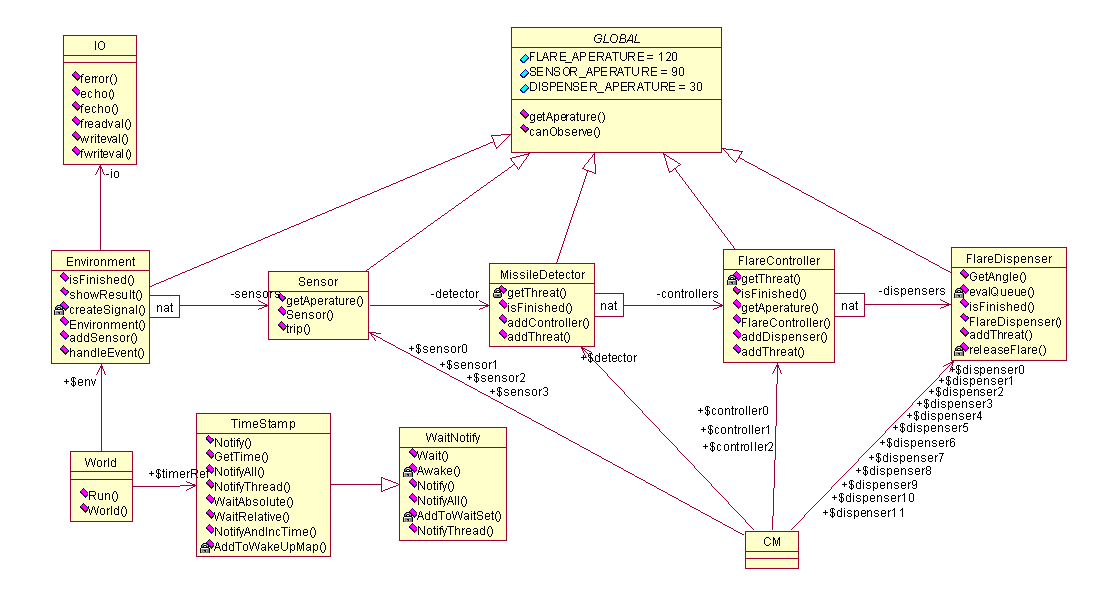
\includegraphics[width=\textwidth]{concurCMclassdiag}
\end{center}
\caption{並列防御対策モデルに対するクラス図\label{fig:classdiagconcur}}
\end{figure}

\subsection{World クラスの変更}

\texttt{timerRef} インスタンス変数は \texttt{Timer} クラスへの参照から\texttt{TimeStamp} クラスへの参照に変更されている。
これは異なる独立なスレッド間で適切に同期を行うために成されている。

 \texttt{World} クラスの構成子は、\texttt{CM}クラスからの静的に宣言された \texttt{detector}へのスタート文が最後におかれていることを除けば、前述のモデルから変更はない。

\begin{lstlisting}
start(CM`detector)
\end{lstlisting}

しかしながら \texttt{Run} 操作は抜本的に変更されたため、以下の通りとなる:

\begin{lstlisting}
public Run: () ==> ()
Run () == 
  (-- start the environment
   start (env);
   -- wait for the environment to handle all input
   env.isFinished();
   -- wait for the missile detector to finish
   CM`detector.isFinished();
   -- print the result
   env.showResult())
\end{lstlisting}

この新しい定義は、望まれたアクション実行の準備が本当に整うまでは遮断されるように定義された許可述語、をもつ様々な操作に、如何に依存しているかについては注意しよう。

\subsection{Environment クラスの変更}

 \texttt{Environment} クラスにおいて、 \texttt{Run} 操作は削除され、その代わりにスレッドが含まれている。
これは次の様になる:

\begin{lstlisting}
thread
  while true do
   (if busy
    then createSignal();
    World`timerRef.NotifyAndIncTime())
\end{lstlisting}

基本的にここでのスレッドは\texttt{Run} 操作と似ているが、少しだけより単純化されている。

 \texttt{isFinished} 操作もまたその述語を許可述語の中に移すことで単純化されている。
最後に、もしそれが既に実行されていれば発動できないことを確実にしている \texttt{handleEvent} 操作に対して、同期化制約が成される(下記の \texttt{sync}章にある \texttt{mutex} 述語)。

\begin{lstlisting}
public isFinished : () ==> ()
isFinished () == skip;

sync

mutex (handleEvent);
per isFinished => not busy;
\end{lstlisting}

\subsection{MissileDetector クラスの変更}

 \texttt{addController} 操作においては、追加された制御装置もまたスタートするため、定義は次の通りとなる:

\begin{lstlisting}
public addController: FlareController ==> ()
addController (pctrl) ==
  (dcl nid : nat := card dom ranges + 1;
   atomic
    (ranges := ranges munion {nid |-> pctrl.getAperture()};
     controllers := controllers munion {nid |-> pctrl}
    );
   start (pctrl) );
\end{lstlisting}

 \texttt{Environment} クラスにおける \texttt{Run}操作に対するの同様に、 \texttt{Step} 操作は削除される。
その代わりにスレッドが導入される。
もし何らかの脅威が現れると、前述の \texttt{Step} が行ったのとまったく同様の方法で、ミサイル検知スレッドは繰り返し脅威を読み込む。

\begin{lstlisting} 
thread

-- the missile detector continuously processes sensor
-- events. getThread is automatically blocked if there
-- are no threats available
while true do
  (def mk_ (evid,pmt, pa, pt) = getThreat() in
     for all id in set dom ranges do
       def mk_(papplhs, pappsize) = ranges(id) in
         if canObserve(pa, papplhs, pappsize)
         then controllers(id).addThreat(evid,pmt,pa,pt);
   busy := len threats > 0 )
\end{lstlisting}

操作 \texttt{isFinished} は逐次モデルとは異なるが、スレッドが終了してしまうまで遮断するための許可述語を用いるからである。
これは \texttt{forall} の定量化を、すべての \texttt{controllers}に及ぶループというように変更することを意味している。

\begin{lstlisting}
public isFinished: () ==> ()
isFinished () ==
  for all id in set dom controllers do
    controllers(id).isFinished()
\end{lstlisting}

同期化の視点から見れば、 \texttt{addThreat} と\texttt{getThreat} は同じインスタンス変数を修正しているため、 \texttt{mutex}述語を用いて互いに排他的に宣言される必要がある。
加えて、\texttt{getThreat} と \texttt{isFinished} の操作に対して許可述語が導入される。
\texttt{getThreat} は、\texttt{MissileDetector}を制御する主たるスレッドからは ``blocking read'' として用いられる。

\begin{lstlisting}
sync

mutex (addThreat,getThreat);

per getThreat => len threats > 0;
per isFinished => not busy
\end{lstlisting}

\subsection{火炎弾制御クラスの変更}

 \texttt{addDispenser} 操作においては、追加された容器もまたスタートするため、定義は次の様になる:

\begin{lstlisting}
public addDispenser: FlareDispenser ==> ()
addDispenser (pfldisp) ==
  let angle = aperture + pfldisp.GetAngle() in
    (dcl id : nat := card dom ranges + 1;
     atomic
      (ranges := ranges munion 
                 {id |-> mk_(angle, DISPENSER_APERTURE)};
       dispensers := dispensers munion {id |-> pfldisp});
     start (pfldisp) );
\end{lstlisting}

 \texttt{MissileDetector} クラスに対するのとまったく同様に、\texttt{Step}操作は削除され代わりに新しいスレッドが導入される。
スレッドでは最初に、制御するすべての容器に対するスレッドをスタートさせることが必要だ。
発射制御装置に対するスレッドは、ある脅威が現れた場合の操作\texttt{Step}の一部と同様である。
\texttt{FlareController} スレッドは継続してセンサー事象を処理する。

\begin{lstlisting}
thread

(while true do
   (def mk_ (evid,pmt, pa, pt) = getThreat() in
      for all id in set dom ranges do
        def mk_(papplhs, pappsize) = ranges(id) in
          if canObserve(pa, papplhs, pappsize)
          then dispensers(id).addThreat(evid,pmt,pt);
    busy := len threats > 0 ) )
\end{lstlisting}

操作 \texttt{isFinished} は逐次モデルとは異なるが、スレッドが終了してしまうまで阻止するための許可述語を用いるからである。
これは \texttt{forall} の定量化を、すべての  \texttt{dispensers}に及ぶループというように変更することを意味している。

\begin{lstlisting}
public isFinished: () ==> ()
isFinished () ==
  for all id in set dom dispensers do
    dispensers(id).isFinished();
\end{lstlisting}

同期化の視点から見れば、 \texttt{addThreat} と\texttt{getThreat} は同じインスタンス変数を修正しているため、上記の \texttt{MissileDetector} クラスに対してと全く同様に \texttt{mutex}述語を用いて互いに排他的に宣言される必要がある。
加えて、\texttt{getThreat} と \texttt{isFinished} の操作に対して許可述語が導入される。
\texttt{getThreat} は\texttt{FlareController}を制御する主たるスレッドからは ``blocking read'' として用いられる。

\begin{lstlisting}
sync

mutex (addThreat,getThreat);

per getThreat => len threats > 0;
per isFinished => not busy
\end{lstlisting}

\subsection{FlareDispenser クラスの変更}

 \texttt{FlareDispenser} クラスにおける \texttt{Step} 操作は、\texttt{FlareController} と \texttt{MissileDetector} のクラスに対するのとまったく同様に、スレッドに変更される。
機能性の大部分は\texttt{evalQueue}という名の新しい操作内におかれている。

\begin{lstlisting}
thread
  while true do
    (World`timerRef.WaitRelative(TimeStamp`stepLength);
     evalQueue());
     
operations

private evalQueue: () ==> ()
evalQueue () ==
  (if len curplan > 0
   then (dcl curtime : nat := World`timerRef.GetTime(),
             done : bool := false;
         while not done do
           (dcl first : PlanStep := hd curplan,
                next : Plan := tl curplan;
            let mk_(fltp, fltime) = first in
              (if fltime <= curtime
               then (releaseFlare(eventid,fltp,fltime,curtime);
                     curplan := next;
                     if len next = 0
                     then (curprio := 0; 
                           done := true; 
                           busy := false ) )
               else done := true ) ) ) );
\end{lstlisting}

前述同様に、 述語を許可述語に変えることで\texttt{isFinished} 操作は変更される。
同期化の視点から見れば、\texttt{mutex}述語が \texttt{addThreat} と\texttt{evalQueue}の操作に対して用いられる。

\begin{lstlisting}
public isFinished: () ==> ()
isFinished () == 
  skip

sync

mutex (addThreat,evalQueue);
per isFinished => not busy
\end{lstlisting}

\subsection{TimeStamp クラスの導入}

 \texttt{TimeStamp} 設計パターンは Appendix~\ref{sec:TimeStamp}で詳細が紹介されている。 
しかし、ここで並列  VDM++ 防御対策モデルで用いられてきた主要な操作が導入される。
 \texttt{TimeStamp} パターンはそのほかの点では独立なスレッド間で同期の処置がとられる保証をするために用いられる (\texttt{TimeStamp}透視からのクライアントとして動作する)。 
 \texttt{TimeStamp} クラスは、  \texttt{WaitNotify}クラスのサブクラスであるが、これはJava \cite{Gosling&00} で用いられている 待機通告メカニズムをモデル化するもので、詳細はAppendix~\ref{app:waitnotify}に記述されている.

\texttt{TimeStamp} は、現時刻を表すものとそれぞれの時に起こされるのはどのスレッドかの情報を表すものとの、2つのインスタンス変数を持つ。

\begin{lstlisting}
class TimeStamp is subclass of WaitNotify

instance variables
  
currentTime : nat := 0;
wakeUpMap : map nat to nat := {|->};
\end{lstlisting}

クライアントは、相対的または絶対的な waitを要請してよいが、並列防御対策モデルにおいては相対的な待ちのみが利用されている。
これは \texttt{WaitRelative}を用いて実行される。

\begin{lstlisting}
operations

public WaitRelative : nat ==> ()
WaitRelative(val) ==
( AddToWakeUpMap(threadid, currentTime + val);
  WaitNotify`Wait();
);
\end{lstlisting}

\texttt{AddToWakeUpMap}は \texttt{wakeUpMap}に新しい待ちを追加するために用いられる。

\begin{lstlisting}
AddToWakeUpMap : nat * nat ==> ()
AddToWakeUpMap(tId, val) ==
  wakeUpMap := wakeUpMap ++ { tId |-> val };
\end{lstlisting}

操作 \texttt{NotifyAndIncTime} は、時刻を増加し現時刻の処置を待っているすべてのスレッドを起動するために、用いられる。

\begin{lstlisting}
NotifyAndIncTime : () ==> ()
NotifyAndIncTime() ==
( currentTime := currentTime + 1;
  for all t in set dom (wakeUpMap :> {currentTime}) do
    NotifyThread(t)
);
\end{lstlisting}

特定のスレッドは\texttt{NotifyThread}を用いて即座に起動できる。

\begin{lstlisting}
public NotifyThread : nat ==> ()
NotifyThread(tId) ==
( wakeUpMap := {tId} <-: wakeUpMap;
  WaitNotify`NotifyThread(tId)
);
\end{lstlisting}

クラスの現在時刻は \texttt{GetTime}操作を通して得られる。

\begin{lstlisting}
public GetTime : () ==> nat
GetTime() ==
  return currentTime;
\end{lstlisting}

 \texttt{wakeUpMap} はたくさんの様々な操作により動かされるので、それらに対し中立的排他的であるためにアクセス設定を行う必要がある。

\begin{lstlisting}
sync

mutex(AddToWakeUpMap, Notify, NotifyThread, NotifyAll);
\end{lstlisting}

%The time stamp thread periodically calls
%\texttt{NotifyAndIncTime}. The period of the thread depends on the
%desired value of one time step.

%\begin{lstlisting}
%thread

%  periodic (1000)(NotifyAndIncTime)

%end TimeStamp
%\end{lstlisting}

\subsection{モデルの妥当性検査}

先に提示した逐次 VDM++ モデルに関して、上記で提示した並列VDM++ モデルの正しい動作についての妥当性検査を行う必要がある。
これらモデルの両方とも入出力に対する標準\texttt{IO} クラスを用いる。
前述同様に、これをスタートするのに、簡単なテストケースの提供から始め、それから徐々により複雑なものにしていく。
並列 VDM++ モデルに利用される入力形式は逐次 VDM++ モデルに利用されるものと同一であるため、様々な\texttt{scenario.txt} ファイルをもつすべてのテストケースで変更なしに再利用されることが可能である。
 \texttt{FlareDispenser}に対して相対的角度をもつ事象がまだ存在し、興味をもたれた読者はこのモデルに対する同種の変更を行うことができる。

逐次 VDM++ モデルに関してWEB上で利用できるこのモデルのインターネット版は、多少複雑な\texttt{scenario.txt}となったが、、\texttt{new World().Run()}を評価することでモデルの全部分を少なくとも一度は練習することを確実にするのに十分なものである。
ここでは\VDMTools のテストカバレージ機能を用いていることを、再度述べておく。

\subsection{要約}

第~\ref{sec:concurmod} 章では、防御対策システムの並列設計指向的モデルが提示された。
このモデルは第~\ref{sec:seqVDM}章にある静的構成要素(クラス)への分解の再利用を行っている。
加えて、動的構造(スレッド)を追加している。
このモデルの長所は、動的な構造の導入であり、一方で機能的に正確な動作を今もなお確実なものとしている。
ここでのモデルの精度が、伝統的な検査技術を用いた妥当性検査を可能にする。

このモデルは、第~\ref{sec:VDMSLreq}章と~\ref{sec:seqVDM}章の VDM-SL モデルと 逐次 VDM++ モデルに対して用いられたテストケースを用いて、テストされた。
この方法で、古いテストケースがシステム受入れテスト中に再利用され、そしてVDM-SL モデルは、この並列 VDM++ モデルの機能的な動作を比較するための1つの助言として、逐次 VDM++ モデルに関するのと同じ方法で用いられた。

この並列設計モデルから学ぶことができるのは、今システムの動的構造の共通な理解をもっているということである。
加えて、 第~\ref{sec:VDMSLreq}章と~\ref{sec:seqVDM}章のより抽象化されたレベルで記述された動作に相当する新しいモデルの機能性、を妥当性検査してきた。
この妥当性検査は再び伝統的な検査技術を用いて行われたし、逐次 VDM++ モデルからのテストケースの莫大な再利用が可能であった。

\section{リアルタイム並列/分散 VDM++ 設計モデル}\label{sec:realtime}

リアルタイムモデルは並列モデルと多くの面で異なっている:

\begin{itemize}
\item  \texttt{World}クラス内の\texttt{timerRef} インスタンス変数は、 VDM++ に対する拡張が直接に時間を含めるため、もはや必要とされていない。
\item  \texttt{CM} クラスはシステムに変更された (\texttt{class} キーワードを \texttt{system} キーワードに変更することで). 
加えて、静的インスタンス変数が \texttt{CPU}と\texttt{BUS}に対して導入され、 システムの機能性の配置が求められている。
最後に、構成子が \texttt{CM} システムに導入され、様々な静的に宣言されたインスタンス変数を様々な\texttt{CPU}に配置する。
\item 単にもう1つのスレッドに信号を送る必要のある並列モデルからのたくさんの操作が、 \texttt{async}キーワードを用いることで非同期に変えられる。
\item Duration文は、以前の経験から実行時間が知られているモデルの部分を指し示すのに、用いることができる。
\item Cycle文は時計周期数が以前の経験から既に知られている部分を指し示すことができる。
\end{itemize}

そうでない場合、モデルは並列モデルから概して変化しない。
様々なクラスの概観は、図~\ref{fig:classdiagvice}で見ることができる。

\begin{figure}
\begin{center}
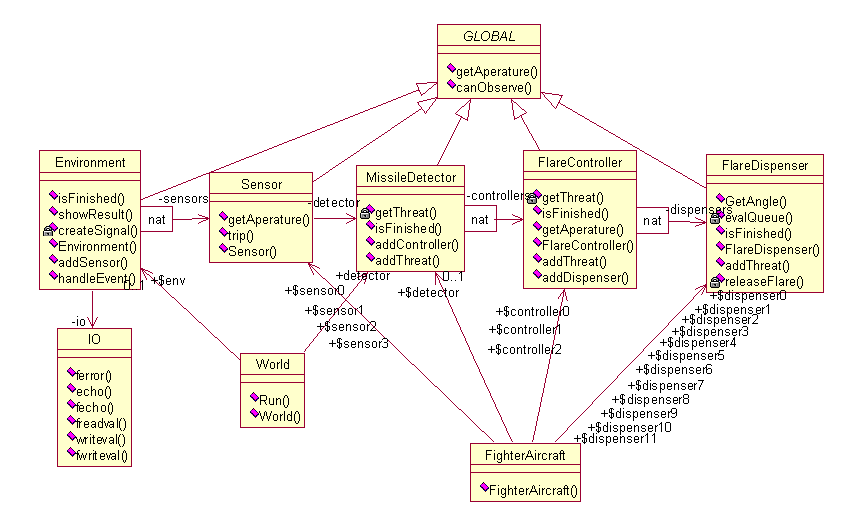
\includegraphics[width=\textwidth]{viceCMclassdiag}
\end{center}
\caption{リアルタイム分散防御対策モデルのためのクラス図\label{fig:classdiagvice}}
\end{figure}

\subsection{防御対策クラスの変更}

上記で説明した通り、 \texttt{CM} クラスはたくさんの新しいインスタンス変数をもつ。
ここで考えられた経験に基づくハードウェア構造は、6つの \texttt{CPU}と3つの \texttt{BUS}をもつ。
これらの宣言は次の様になる: 

\begin{lstlisting}
instance variables
cpu1 : CPU := new CPU (<FCFS>,1E6);
cpu2 : CPU := new CPU (<FCFS>,1E6);
cpu3 : CPU := new CPU (<FP>,1E9);
cpu4 : CPU := new CPU (<FCFS>,1E6);
cpu5 : CPU := new CPU (<FCFS>,1E6);
cpu6 : CPU := new CPU (<FCFS>,1E6);
bus1 : BUS := new BUS (<FCFS>,1E6,{cpu1,cpu3});
bus2 : BUS := new BUS (<FCFS>,1E6,{cpu2,cpu3});
bus3 : BUS := new BUS (<FCFS>,1E6,{cpu3,cpu4,cpu5,cpu6});
\end{lstlisting}

このハードウェア構造のグラフィカルな概観は、 \texttt{showtrace} 外部ツールを用いて自動的に生成される。
この多少複雑な構造のため、 図~\ref{fig:cpuarchitecture}のように見える。

\begin{figure}
\begin{center}
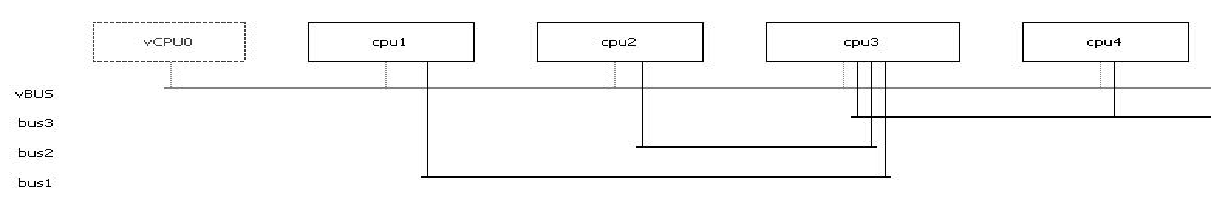
\includegraphics[width=\textwidth]{cpuarchitecture}
\end{center}
\caption{分散型防御対策モデルのためのCPU 構造
\label{fig:cpuarchitecture}}
\end{figure}

\texttt{CM} 構成子はそれから、すべての静的なインスタンスをこれら様々な \texttt{CPU}に配置し、各々の \texttt{CPU}で用いられた多くの操作に対して優先順位を設定する。

\begin{lstlisting}
operations

public CM: () ==> CM
CM () ==
  (cpu3.deploy(detector);
   cpu3.setPriority(MissileDetector`addThreat,100);
   cpu1.deploy(sensor0);
   cpu1.setPriority(Sensor`trip,100);
   cpu1.deploy(sensor1);
   cpu2.deploy(sensor2);
   cpu2.setPriority(Sensor`trip,100);
   cpu2.deploy(sensor3);
   cpu3.deploy(controller0);
   cpu3.setPriority(FlareController`addThreat,80);
   cpu4.deploy(dispenser0);
   cpu4.setPriority(FlareDispenser`addThreat,100);
   cpu4.setPriority(FlareDispenser`evalQueue,80);
   cpu4.deploy(dispenser1);
   cpu4.deploy(dispenser2);
   cpu4.deploy(dispenser3);
   cpu3.deploy(controller1);
   cpu5.deploy(dispenser4);
   cpu5.setPriority(FlareDispenser`addThreat,100);
   cpu5.setPriority(FlareDispenser`evalQueue,80);
   cpu5.deploy(dispenser5);
   cpu5.deploy(dispenser6);
   cpu5.deploy(dispenser7);
   cpu3.deploy(controller2);
   cpu6.deploy(dispenser8);
   cpu6.setPriority(FlareDispenser`addThreat,100);
   cpu6.setPriority(FlareDispenser`evalQueue,80);
   cpu6.deploy(dispenser9);
   cpu6.deploy(dispenser10);
   cpu6.deploy(dispenser11);
   )
\end{lstlisting}

\subsection{World クラスの変更}

 \texttt{World} クラスにおける変更はただ\texttt{timerRef}インスタンス変数が削除されたことである。

\subsection{Environment クラスの変更}

\texttt{timerRef} 参照を用いる代わりに、ここでは\texttt{Environment} クラスが 特別な \texttt{time}キーワードを使用する。
これは例えば操作\texttt{createSignal} において見ることができるが、ここでは \texttt{duration} 文もまた導入されている。

\begin{lstlisting}
private createSignal: () ==> ()
createSignal () ==
  duration (10) 
  (if len inlines > 0
   then (dcl curtime : nat := time, done : bool := false;
         while not done do
           def mk_ (eventid, pmt, pa, pt) = hd inlines in
             if pt <= curtime
             then (for all id in set dom ranges do
                     def mk_(papplhs,pappsize) = ranges(id) in
                       if canObserve(pa,papplhs,pappsize)
                       then sensors(id).trip(eventid,pmt,pa);
                   inlines := tl inlines;
                   done := len inlines = 0;
                   evid := eventid )
             else (done := true;
                   evid := nil))
   else (busy := false;
         evid := nil));
\end{lstlisting}

これ以外に新しい \texttt{Environment} クラスに対する唯一の相違は、スレッドが周期的に作られることである:

\begin{lstlisting}
thread

periodic (1000,10,900,0) (createSignal)
\end{lstlisting}

\subsection{Sensor クラスの変更}

 \texttt{Sensor}クラスに対して唯一必要な変更は、\texttt{trip} 操作が非同期になされること、そして\texttt{time} キーワードを \texttt{World`timerRef.GetTime()} 式の代わりかわりに用いることである。
このようにして、現在 the \texttt{trip} 操作は次のように見える:

\begin{lstlisting}
async public trip: MissileType * Angle ==> ()
trip (pmt, pa) ==
  -- log and time stamp the observed threat
  detector.addThreat(pmt,pa,time)
pre canObserve(pa, aperture, SENSOR_APERTURE)
\end{lstlisting}

\subsection{ミサイル検知クラスの変更}

 \texttt{MissileDetector} クラスに対して唯一必要な変更は、\texttt{addThreat} 操作が非同期になされることである。

\subsection{FlareControllerクラスの変更}

 \texttt{MissileDetector} クラスに対するのとまったく同じに、 \texttt{FlareController} クラスに対して唯一必要な変更は\texttt{addThreat} 操作が非同期になされることである。

\subsection{FlareDispenser クラスの変更}

 \texttt{FlareDispenser} クラスで、 \texttt{addThreat} と\texttt{evalQueue} 操作は非同期でなされる。
加えて、上記のわずかな他のクラスに対すると同様に、ここで\texttt{time} キーワードに対して直接に参照を行う。
このように、これら2つの操作は現在以下のように見れる:

\begin{lstlisting}
async public addThreat: EventId * MissileType * nat ==> ()
addThreat (evid, pmt, ptime) ==
  if missilePriority(pmt) > curprio
  then (dcl newplan : Plan :=  [],
            newtime : nat := ptime;
        -- construct an absolute time plan
        for mk_(fltp, fltime) in responseDB(pmt) do
          (newplan := newplan ^ [mk_ (fltp, newtime)];
           newtime := newtime + fltime );
        -- immediately release the first action
        def mk_(fltp, fltime) = hd newplan in
          releaseFlare(evid,fltp,fltime,time);
        -- store the rest of the plan
        curplan := tl newplan;
        eventid := evid;
        curprio := missilePriority(pmt);
        busy := true );

async evalQueue: () ==> ()
evalQueue () ==
  duration (10)
  (if len curplan > 0
   then (dcl curtime : nat := time, done : bool := false;
         while not done do
           (dcl first : PlanStep := hd curplan,
                next : Plan := tl curplan;
            let mk_(fltp, fltime) = first in
              if fltime <= curtime
              then (releaseFlare(eventid,fltp,fltime,curtime);
                    curplan := next;
                    if len next = 0
                    then (curprio := 0; 
                          done := true; 
                          busy := false ) )
              else done := true ) ) );
\end{lstlisting}

加えて、スレッドは\texttt{Environment} クラスに対したのと同様に周期的に作成される。

\begin{lstlisting}
thread

periodic (1000,0,0,0) (evalQueue)
\end{lstlisting}

\subsection{モデルの妥当性検査}

 以前に提示されたVDM モデルに対すると同様、上で提示されたリアルタイム分散VDM++ モデルの正しい動作を妥当性検査する必要がある。
これらモデル両方は、入出力に対して標準\texttt{IO} クラスを用いる。
前述と同様に、妥当性検査は簡単なテストケースの提供から始め、徐々により複雑なものを対象とすることになるだろう。
リアルタイム分散 VDM++ モデルのため用いる入力形式は並列 VDM++ モデルのために用いるものと一致しているため、テストケース各々の\texttt{scenario.txt} ファイルを用いる妥当性検査では、全テストケースが少しの変更もなく再びの再利用が可能である。
しかし、ここでは時間計測のおかげでこのシステムの ``real-world''実装に近づいているので、出力の期間計測は以前のモデルのものとは一致しないことを期待する必要がある。
したがって時間計測が何らかのボトルネックを引き起こすかどうかの判断は、指示子しだいである。
もう1つ、\texttt{FlareDispenser}に対する相対的角度を論点にするものもまだ存在するので、興味を持たれる読者はこのモデルに対して同種の変更を行うことができる。

前述の VDM++ モデルに関してWEB上で利用できるこのモデルのインターネット版は、多少複雑な\texttt{scenario.txt}となったが、、\texttt{new World().Run()}を評価することでモデルの全部分を少なくとも一度は練習することを確実にするのに十分なものである。
ここでは\VDMTools のテストカバレージ機能を用いていることを、再度述べておく。

\subsection{要約}

この章では、タイミング情報を組み入れて分散型構造を提供する防御対策システムのモデルを提示してきた。
ある程度はこのモデルはまだ現実世界の理想化である、ことは指摘しておくべきであろう。
モデルは決定論的であり、ハードウェアは完全に実行を行い、指定された間隔以内で応答する、と仮定する。起きるかもしれない何らか外部事象にも限定された見方しか行わない。 
これらは2つの理由から、提案されたアプローチにおける重要な流れではない。

\begin{itemize}
\item 例えば\ 決定主義やハードウェア動作に関してなされる多くの仮定は、またホスト統合テストの間にもなされる;
これらの仮定が破られたときのシステム動作は、対象の統合テストの間にのみテストできる。
\item 
原則的に、あらゆる種類の事象をモデル化することが可能である。
特に``unknown'' 事象、またこのような事象の存在の中に記述されるシステム動作、がモデル化できるであろう。
\end{itemize}

\chapter{同期}\label{chap:sync}

この章では、並列スレッドに関連する事項が追加されている。
特に、共有オブジェクトに対して同期を記述するための原則が述べられ、さらにはこれらの原則に基づく同期のメカニズムが示される。

\section{同期の原則}

VDM++における同期は、\emph{permission predicates}を用いて行われる。
許可述語は、そこで操作が実行されるかもしれない環境を指定する式である。

\begin{lstlisting}
per @\emph{operation name}@ => @\emph{guard condition}@
\end{lstlisting}

許可述語の意味論としては、クライアントが操作呼び出しを要求する時にその操作の許可述語が評価される、というようなことになる。
もしこれが真であるとしたら、実行が始まって操作が起動されるのかもしれない; もし誤りであるのなら、クライアントが遮断されることでスケジューラが起動されるのである。
許可述語は、クラスの sync 節に一覧されている。
便利な省略形として、キーワードである \texttt{mutex} を用いて操作間の相互排除を表現してもよい。
さらなる詳細については、様々な種類の保護条件と共に以下に述べる。

保護条件は、そのクラスのインスタンス変数に全体に及ぶ作用領域を持っている。
例えば、単一バッファの以下の仕様を考えてみよう:
\newpage

\begin{multicols}{2}
\begin{lstlisting}
class Buffer

instance variables
  data : [nat] := nil

operations
  public Put : nat ==> ()
  Put(v) == data := v;

sync
  per Put => data = nil;
\end{lstlisting}
\begin{lstlisting}
  public Get : () ==> nat
  Get() ==
   let n = data in
     (data := nil;
      return n)
  pre data <> nil

sync
  per Get => data <> nil

end Buffer
\end{lstlisting}
\end{multicols}

\subsection{履歴カウンタ}

保護条件ではまた \emph{history counters}の参照が可能である。
これは特定の操作の履歴を記述するものだ。
基本となる3つの履歴カウンタがある:

\begin{description}
\item[\texttt{\#req(op)}] ある特定のオブジェクトにおいて op が要求された回数;
\item[\texttt{\#act(op)}] ある特定のオブジェクトにおいて op が発動された回数;
\item[\texttt{\#fin(op)}] ある特定のオブジェクトにおいて op が実行を完了した回数\end{description}

簡単な例題として、N台設置バッファを考えてみよう:

\begin{multicols}{2}
\begin{lstlisting}
class BufferN

values
  N : nat = 5

instance variables

  data : seq of nat := [];
  inv len data <= N

operations
  public Put : nat ==> ()
  Put(v) ==
    data := data ^ [v];

\end{lstlisting}
\begin{lstlisting}
  public Get : () ==> nat
  Get() ==
    let n = hd data in
      (data := tl data;
       return n)
  pre data <> []

sync
  per Put =>
    #fin(Put) - #fin(Get) < N;
  per Get =>
    #fin(Get) < #fin(Put);

end BufferN
\end{lstlisting}
\end{multicols}

この例題では、複数の許可述語がそのクラスのインスタンス変数に関して、同等によく表現され得ていることに注意したい。
しかしながら、一般的にこのような保護においては、もっと洗練された同期述語の使用が可能である。
例えば、 常に \texttt{Put} のN個の起動のみを動作中とできる、という要求を表現することができる:

\begin{lstlisting}
per Put => #fin(Put) - #fin(Get) < N and #fin(Put) = #act(Put);
\end{lstlisting}

基本的な履歴カウンタに加え、派生した2つの履歴カウンタがある:

\begin{description}
\item[\texttt{\#active(op)}]  opの現在作動中のインスタンス数。したがって \\ \texttt{\#active(op) = \#act(op) - \#fin(op)}。
\item[\texttt{\# waiting(op)}]  opに対するまだ作動していない要求数。したがって \\ \texttt{\#waiting(op) = \#req(op) - \#act(op)}。
\end{description}

\subsection{相互排除}

基本履歴カウンタを用いて、複数の操作起動間に相互排除 (\emph{mutex}) を指定することが可能だ。
しかしながら、 \texttt{mutex} 述語の省略形としてキーワード \texttt{mutex} を使用できればというのが共通の要求となるであろう。

\texttt{mutex} 述語はユーザーが、そのクラスの全ての操作が相互排除をしながら実行される、あるいは一覧の操作が互いに相互排除的に実行される、ことを指定できるようにする。
1つの相互排除述語に現れる操作は、他の \texttt{mutex} 述語でも同様に現れることができて、また通常の許可述語にて用いられることも可能だ。
各々の \texttt{mutex} 述語は暗黙に、名前一覧に載る各々の操作に対する履歴保護を用いることで、許可述語に翻訳される。
たとえば、

\begin{lstlisting}
sync
  mutex(opA, opB);
  mutex(opB, opC, opD);
  per opD => someVariable > 42;
\end{lstlisting}

これは以下のような許可述語 (上記の式と意味論的に同等である)に翻訳されるだろう:

\begin{lstlisting}
sync
  per opA => #active(opA) + #active(opB) = 0;
  per opB => #active(opA) + #active(opB) = 0 and
             #active(opB) + #active(opC) + #active(opD) = 0;
  per opC => #active(opB) + #active(opC) + #active(opD) = 0;
  per opD => #active(opB) + #active(opC) + #active(opD) = 0 and
             someVariable > 42;
\end{lstlisting}

各々のクラスで各々の操作に対して、1つの明白な許可述語をもつことだけは唯一許されていることに注意しよう。

\texttt{mutex(all)}束縛では、 そのクラス \emph{および任意のスーパークラスで} で指定された操作の全ては互いに排他的に実行されるべきであることを示している。

\texttt{mutex}を使用することで、危険域の並列実行を防ぐことができることは明らかである。

\section{待機通告}\label{sec:waitnotify}

よく知られている同期のメカニズムは、Java プログラミング言語 \cite{Gosling&00}に用いられている待機通告である。
この概念を理解するために、次に定義される \texttt{b} という同期は行われていない共有バッファによって伝達を行う2つのスレッド \texttt{Producer} と\texttt{Consumer} を考えてみよう。

\begin{multicols}{2}
\begin{lstlisting}
class UnsyncBuffer

instance variables
  data : [nat] := nil

operations
  public Put : nat ==> ()
  Put(v) ==
    data := v;
\end{lstlisting}
\begin{lstlisting}

  public Get : () ==> nat
  Get() ==
    let n = data in
      (data := nil;
       return n)
  pre data <> nil

end UnsyncBuffer
\end{lstlisting}
\end{multicols}

非同期のバッファは、プロデューサとコンシューマのスレッド間でデータ交信を行うために用いられる。

\begin{multicols}{2}
\begin{lstlisting}
-- Producer thread
while true do
  (let v = Produce() in
     b.Put(v))
\end{lstlisting}
\begin{lstlisting}

-- Consumer thread
while true do
  Consume(b.Get())
\end{lstlisting}
\end{multicols}

もちろん、コンシューマスレッドがデータをコンシューマする場合に有効なデータがバッファに必ずしも存在する必要はない、という問題がおきる。
さらに、プロデューサスレッドがコンシューマスレッドに対して ``too fast''なデータを生成するとデータが失われる可能性がある。

待機通告オブジェクトは、バッファに対するアクセスを2つのスレッドを通して同期させることを可能とする。

\begin{multicols}{2}
\begin{lstlisting}
-- Producer thread
while true do
  (let v = Produce() in
     b.Put(v)
   o.Notify();
   o.Wait())
\end{lstlisting}
\begin{lstlisting}

-- Consumer thread
while true do
  (o.Wait();
   Consume(b.Get());
   o.Notify())
\end{lstlisting}
\end{multicols}

1つのスレッドは\texttt{o.Wait}を呼び出した後は、もう1つのスレッドが \texttt{o.Notify}を呼び出すまで遮断する。
このようにこの例題で、産出スレッドは値の産出後はこれをバッファに置き、コンシューマスレッドに通告し、そして遮断する。
コンシューマスレッドはプロデューサスレッドに通告されるまでは遮断されているが; それからバッファ内のデータをコンシューマし、その後にプロデューサスレッドに通告する。

待機通告を用いることの利点は、任意の共有オブジェクトに対するアクセスを同期させることに用いることができるということであり; つまりは、この共有オブジェクトは共有ということを頭に入れて設計される必要がなかったということである。
このことは大いに仕様と設計を簡略にするものであり、なぜなら動的構造設計が始まるまでは同期の考慮を支障なく延期することができるからである。

待機通告メカニズムの初期化には配慮のなされる必要があるが、これはデッドロックを起こす可能性があるからである。
例えば上記の例題では、もしプロデューサスレッドが最初に実行されたならば、その通告に続いてプロデューサとコンシューマの両方が新たな通告を待っていることとなり、これが外から与えられなければならない。
代わりに、スレッドは最初に実行されるようコンシューマを強要するような方向に編成されることが可能だ。

待機通告はVDM++における原則ではなく; むしろユーザー定義クラスである、ということに注意しよう。
この定義は Appendix~\ref{app:waitnotify}で見つけられる。

\section{スレッド完了}

許可述語の一般的な使用としては、他のすべてのスレッドの完了まで既定スレッドを遮断することがある。
たとえば、図~\ref{fig:notwait}のモデルを考えよう。

\texttt{Main} は実行時に\texttt{SubThread}のインスタンスを生成しスタートするが、\texttt{SubThread} が必要に応じて何らかのデータをここにおく機会を得る前に、共有オブジェクトの内容を引き渡すのである。

この問題を解決するためには、完了を決定するために共有オブジェクトが用いられるべきである。
操作 \texttt{IsFinished}が \texttt{Shared}の仕様に追加されるべきである。
この操作の呼び出しは、 \texttt{SubThread} が完了したと決定されるまで、遮断するべきである。

\begin{figure}
\begin{multicols}{2}
\begin{lstlisting}
class Shared

instance variables
  data : seq of nat := []

operations
  public Put : nat ==> ()
  Put(n) ==
    data := data ^ [n];

  public Get : () ==>
               seq of nat
  Get() == return data

sync

mutex(Put);
mutex(Put,Get)

end Shared

class SubThread

instance variables
  s : Shared

operations
\end{lstlisting}
\begin{lstlisting}

  public Init : Shared ==> ()
  Init(ns) == s := ns

thread
  for i = 1 to 100 do
    s.Put(i * i)

end SubThread

class MainThread

operations

  public Main :
           () ==> seq of nat
  Main() ==
    (dcl s : Shared :=
               new Shared(),
         t : SubThread :=
               new SubThread();
     t.Init(s);
     start(t);
     return s.Get() 
    )

end MainThread
\end{lstlisting}
\end{multicols}
\caption{スレッド完了を待たない\label{fig:notwait}}
\end{figure}

操作 \texttt{Main} に対する仕様はしたがって次のようになる:

\begin{lstlisting}
public Main : () ==> seq of nat
Main() ==
  ( dcl s : Shared := new Shared(),
        t : SubThread := new SubThread();
    t.Init(s);
    start(t);
    s.IsFinished();
    return s.Get()
  )
\end{lstlisting}

スレッド完了の決定の遂行は、暗黙にも明示的にも可能である。
暗黙のアプローチは、スレッドにより生成されたデータの総量に基づく。
例えばスレッドが 100個の値を生成することが分かっている場合は、これを完了の決定に用いることができる。

\begin{multicols}{2}
\begin{lstlisting}
class Shared

instance variables
  data : seq of nat := []

operations
  public Put : nat ==> ()
  Put(n) ==
    data := data ^ [n];

  public Get :
          () ==> seq of nat
  Get() == return data;
\end{lstlisting}
\begin{lstlisting}

  public IsFinished :
            () ==> ()
  IsFinished() == skip;

sync

mutex(Put);
mutex(Put,Get);
per IsFinished =>
    #fin(Put) = 100

end Shared
\end{lstlisting}
\end{multicols}

明示的なアプローチにおいては、ずっと待ち続けているスレッドは、共有オブジェクトにその完了を伝える:
\newpage

\begin{multicols}{2}
\begin{lstlisting}
class Shared

instance variables

  data : seq of nat := [];
  finished : bool := false;

operations

  public Put : nat ==> ()
  Put(n) == data := data ^ [n];

  public Get :
          () ==> seq of nat
  Get() == return data;

\end{lstlisting}
\begin{lstlisting}
  public IsFinished :
           () ==> ()
  IsFinished() == skip;

  public Finished : () ==> ()
  Finished() ==
    finished := true

sync
  mutex(Put);
  mutex(Put,Get);
  mutex(Finished);
  per IsFinished => finished

end Shared
\end{lstlisting}
\end{multicols}

\section{要約}

この章では、同期のための様々なメカニズムを提示してきた: 許可述語を用いた同期原則および待機通告メカニズムである。
一般的に許可述語に基づく同期は強力な効果を発揮できるが、この述語が高度な表現に富むものだからである。
この力の代償は、このような許可述語が用いられた場合にデッドロックに悩まされるモデルのデバッグがたいへん難しくなるはずだということだ。
したがって、待機警告メカニズムが用いることが可能な場所どこにでも、デバッグが容易であるので、待機警告クラスの操作内部にどのような問題であるかの同定を助けるためのブレークポイントをおけるようにすることが推奨される。


\chapter{周期性}\label{chap:period}

多くのリアルタイムシステムは周期性の要素 -- 固定頻度での繰り返しを行うもの -- を備えている。
この章では、周期性がどのようにモデル化できるかについて述べる。

\section{周期的スレッド}\label{sec:periodthread}

スレッドは周期的である可能性がある: つまり、操作は固定頻度で呼び出される可能性がある。 
この典型的な使用として、外部センサーの調査を行うということがある。

\begin{lstlisting}
class Sensor

operations
  public GetData : () ==> nat
  GetData() ==
    is not yet specified

end Sensor

class SensorPoll

instance variables
  lastReading : [nat] := nil;
  sensor : Sensor

operations
  public Init : Sensor ==> ()
  Init(ns) ==
    sensor := ns;

  PollSensor : () ==> ()
  PollSensor() ==
    lastReading :=
       sensor.GetData()

thread
  periodic (100,10,90,0) (PollSensor)

end SensorPoll

class Main

operations
  public Run : () ==> ()
  Run() ==
  ( dcl sp : SensorPoll :=
              new SensorPoll(),
        s : Sensor := new Sensor();
    sp.Init(s);
    start(sp)
  )

end Main
\end{lstlisting}

ここでセンサースレッド \texttt{sp} は \texttt{start(sp)}文の実行に続いて、およそ100単位時間に1回の割合で実行されるとする。

上記のような簡単なシステムで、\texttt{PollSensor} はおよそ100単位時間に1回の割合で起動されるはずであることに注意したい。
周期文に対する2番目のパラメータでは、このスレッドの周期的発動に最高10単位時間のジッターが許されていることを示す。
3番目のパラメータは、この周期的スレッドの2つのインスタンス間は少なくとも90単位時間あることを示している。
おしまいに最後のパラメータはこの周期的スレッドの発動に補正は要求されていないことを示す。
たくさんのスレッドが同時にスタートし、それらを特別な順に実行したいというような場合に、これは最も価値のある特性となる。

さらに多くのスレッドをもつシステムにおいて、周期性は単にスケジューラに、特定の周期スレッドがスケジュール化可能な時刻がいつかという情報を与えるだけのことである。
このように実際には、周期的スレッドは遅らされる可能性もある。
事実、周期的スレッドが遅れるというのはしばしばモデルの興味あるプロパティであり、そのモデルのそういった部分は再設計される必要があることを示すはずであるからだ。
したがってタイムトレースファイルにおいて、周期的スレッドが遅れたとすれば、特別な事象は出力である。

\subsection{周期的スレッドとスケジュール化}

Periodic threads are subject to the same scheduling policy as other
threads. This has a number of implications for their
use. Specifically:
周期的スレッドは、他のスレッドと同様のスケジュール化方式に制約されている。
このことが使用に際しては多くを意味する。
具体的には次の通り:

\begin{itemize}
\item たとえある周期的なスレッドがその周期の最後までに完了しなかったとしても、もう1つの周期的スレッドは次の周期で可能となるであろう。
このように、周期的スレッドの同時に重複した発動が可能である。
しかし、ユーザーとしてはこのような使用には慎重になるべきである、というのはもっともっと多くのスレッドが産生されるかもしれないことを意味するからである。
\item 周期に基づくスケジュール化の下では、より高い優先度をもつスレッドがスケジュール化されるため、周期スレッドはその期限を守れない可能性がある。
\end{itemize}

\section{周期的事象のモデル化}\label{sec:modperevents}

一般的には、操作の発動としては外部事象がモデル化される。
このように周期事象をモデル化するには、周期的操作の発動としてモデル化されるべきである。
たとえば、時計をモデル化することを望むと仮定する:

\begin{lstlisting}
class Clock

instance variables
  curtime : nat := 0

operations
  public GetTime : () ==> nat
  GetTime() == return curtime;

  Tick : () ==> ()
  Tick() == curtime := curtime + 1

thread
  periodic (100,0,0,0)(Tick)

end Clock
\end{lstlisting}

 \texttt{Clock} のインスタンスは、100単位時間ごとに実行されるスレッドをもっている。
このような時計はいくつかのスレッド間で共有され、共有スレッドを横切る動作を同期させるために用いられる。
時計の例題としては他に第~\ref{sec:timerclass}章と Appendix~\ref{sec:TimeStamp}に見つけることができるだろう。

\section{統計的スケジュール化可能システム}

特定期間で統計的スケジュール化可能として知られているシステムは、周期的スレッドを用いて簡単にモデル化することができる。
たとえば、それぞれ 30、 70、 110 の単位時間の頻度の3つのスレッド \texttt{A}、\texttt{B}、\texttt{C}を仮定する。

\begin{lstlisting}
class A
...
thread
  periodic (30,0,0,0) (OpA)
end A

class B
...
thread
  periodic (70,0,0,0) (OpB)
end B

class C
...
thread
  periodic (110,0,0,0) (OpC)
end C

class Main

operations
  public Run : () ==> ()
  Run() ==
  ( dcl a : A := new A(),
        b : B := new B(),
        c : C := new C();
    ...
    duration (0)
    startlist({a,b,c});
    ...
  )
end Main
\end{lstlisting}

ここで \texttt{duration(0) startlist(...)} 文は、3つのスレッドすべてがスタート可能な時間は同じであることを保証するために用いられる。
あるスレッドを他のものより遅くスタートさせることを望むのであれば、その1つに対し正の補正値を設定することが可能であろう。

\section{要約}

周期性を見せるシステムは、 言語原則を用いることで、VDM++ で素直に記述することができる。
これらの原則に基づいたタイマーや時計といった特性は、モデルに組み入れることが可能である。

一般的に、システムが統計的にスケジュール化可能であり高いCPU利用要求は持たない場合は、単調比率分析 \cite{Audsley&93,Burns95} がシステムのスケジュール化に用いられる可能性がある。
この場合、指定された期限越えるといった問題は自動的に解決し、よってこのようなシステム単調比率分析が好ましいことによる。

%\fbox{More examples with offset should be introduced!!!!}

\chapter{スケジュール化方式} \label{chap:schedule}

\vdmtools\ は多くの様々なスケジュール化方式をサポートしている。
この章では、これらの様々な方針について述べ、各々特定の方針をもつモデルに対する意味づけをまとめる。

実行中の任意の時点で、\vdmtools\ は2つの補完的スケジュール化方式をとる: 基本スケジュール化方式と第2スケジュール化方式である。

基本スケジュール化方式はいつスレッドがスケジュール解除されるかを決める。
第2のスケジュール化方式は、スケジューラがスケジュールする次のスレッドを見つけようとする順を決定する。
各々のカテゴリを別々に考慮する。

\section{主要なスケジュール化アルゴリズム}

\vdmtools\ は限定された時間と協同の間での基本的スケジュール化アルゴリズムの選択を提供する。
一般的に、許可述語が誤りであるものに対して、スレッドが遮断する時点で、あるスレッドは操作呼出しがなされるまで実行が行われる。

協同スケジュール化アルゴリズムにおいては、スレッドがスケジュール解除されるかもしれない方法は他になく: 各々のスレッドは完了するために実行が許される。

時間の限定されたスケジュール化アルゴリズムにおいては、ある定義された期間以上連続実行が許されるスレッドはない; この期間が完了したときはスケジューラがスレッドのスケジュール解除を行う。

2つの時間限定スケジュール化アルゴリズム:\emph{instruction number scheduling} と \emph{time slice scheduling}が利用できる。
命令番号スケジュール化の下では、各々のスレッドが実行する時間の合計は、スレッドの実行中に実行された命令数により限定される。
このように命令番号スケジュール化の下では、スケジューラによりなされる決定はDuration文または既定継続情報から独立している。
時間分割スケジュール化の下では、各々のスレッドが実行する時間の総計は固定されたシミュレート時刻の総計により制限されている。
このように、このスケジュール化アルゴリズムの下で、各々のスレッドが実行する時間の総計はDuration文に、あるいは既定継続情報に、影響される。

\section{第2のスケジュール化アルゴリズム}

2つのスケジュール化アルゴリズムがサポートされていて: ラウンドロビンまたは優先度に基づくものである。

\subsection{ラウンドロビンスケジュール化}

ラウンドロビンの下では、スケジューラは任意の、固定順、を用いるが、次の実行スレッドを見つけるためのものである。
以下に続く例題を考える。
スレッド \texttt{t1}、 \texttt{t2}、\texttt{t3}と、スケジューラが \texttt{[t1,t2,t3]}の順を用いことを、仮定しよう。 
さらに、 \texttt{t1} がスケジュール解除され、この時点で \texttt{t2} が遮断され、 \texttt{t3} がスケジュール化可能であると仮定しよう。

スケジューラは最初に \texttt{t2} がスケジュール化可能であるかをテストするであろう;
これは遮断がなされているからで、次には \texttt{t3} がスケジュール化可能かをチェックするだろう。
このようにして \texttt{t3}がスケジュール化される。

そして \texttt{t3} がスケジュール解除されたときに、 \texttt{t1} と\texttt{t2} の両方がスケジュール化可能である、と仮定する。
スケジューラは最初に\texttt{t1}を検査し、これはスケジュール化可能なので、選択され実行される。

このようにラウンドロビンスケジュール化の下では、弱い公正プロパティが存在し\cite{Lamport91}: 絶対遮断されないスレッドはそのうちスケジュール化されるであろう。

\subsection{優先度に基づくスケジュール化}

優先度に基づくスケジュール化はラウンドロビンスケジュール化の改良型である。
それぞれのスレッドに対して数の優先度が割り当てられる。
スケジューラーがスケジュールされるべき次のスレッドの選択が必要なときは、優先度が最高のスレッドすべてが標準のラウンドロビンを用いてチェックされる; もしスケジュール化可能なスレッドが見つからなければ、2番目に高い優先度のすべてのスレッドが標準ラウンドロビンを用いてチェックされ、それが続けられる。

これを描くために、以下の例題を考えよう。
スレッド \texttt{a1}、 \texttt{a2}、 \texttt{a3}、 \texttt{b1}、
\texttt{c1}、\texttt{c2}、を仮定する。 
スレッド \texttt{a1}、 \texttt{a2} 、\texttt{a3} の優先度は3; \texttt{b1} は優先度が2、そして\texttt{c1} と \texttt{c2} は優先度1をもつ。
用いられるラウンドロビン順は以下の通りと仮定する:

\begin{tabular}{cl}
Priority & Order \\ \hline
3        & \texttt{[a1,a2,a3]} \\
2        & \texttt{[b1]} \\
1        & \texttt{[c1, c2]} \\
\end{tabular}

以下の状態でスケジュール化を考えよう:

\begin{tabular}{cl}
Thread & Status \\ \hline
a1 & Blocked \\
a2 & Schedulable \\
a3 & Schedulable \\
b1 & Schedulable \\
c1 & Schedulable \\
c2 & Schedulable \\
\end{tabular}

スケジューラは最初に最高優先度のスレッドを調べる。
このように最初のスレッド \texttt{a1} がチェックされるはずだが; これは遮断されたために \texttt{a2}がチェックされる。 \texttt{a2} はスケジュール化可能であるため、選択されるであろう。

またもう1つの状況を考える:

\begin{tabular}{cl}
Thread & Status \\ \hline
a1 & Blocked \\
a2 & Blocked \\
a3 & Blocked\\
b1 & Blocked\\
c1 & Blocked\\
c2 & Schedulable\\
\end{tabular}

スケジューラは最初に優先度3のスレッドを調べる; それらはすべて遮断されている。
それから優先度2のスレッドを調べる; これらもすべて遮断されている。
最後に優先度1のスレッドを調べる: 始めは \texttt{c1}を調べて遮断されているため、\texttt{c2} がチェックされる。
 \texttt{c2}がスケジュール化可能であるためこれが選択される。

優先度が最高ではないスレッドに対しての公式プロパティはなく: それらは渇望される可能性があることに注意したい。

\subsection{既定スレッドの優先度}

 図~\ref{fig:priodefault}にある以下のモデルを考えてみよう。

 \vdmtools\ インタープリタにおいて、ラウンドロビンスケジュール化を用いた式 \texttt{new B().Main()} が実行されることを仮定する。
そしてモデルが実行され、少なくとも11個の要素をもったシーケンスからなる結果が引き渡される。
インタープリタ内で命令が発せられ初期化されたスレッドは、既定スレッドと呼ばれる。
ここで、 \texttt{A}は優先度が2で\texttt{B}は優先度が1であるような、優先度に基づくスケジュール化を用いてモデルが実行される状態を考えてみよう。
この場合は計算が永遠に終了しない、なぜなら \texttt{B} は常にスケジュール化可能である\texttt{A}より低い優先度をもつことでスケジュールされることは決してないからである。

\begin{figure}
\begin{lstlisting}
class A

instance variables
  data : seq of nat := []

operations
  public IsFinished:() ==> ()
  IsFinished() == skip;

  public Get: () ==>
              seq of nat
  Get() == return data

sync
  per IsFinished =>
      len data > 10

thread
  (dcl i : nat := 0;
   while true do
   ( data := data ^ [i];
     i := i + 1 ))

end A

class B

operations
  public Main:() ==> seq of nat
  Main() ==
  ( dcl a : A := new A();
    start(a);
    a.IsFinished();
    a.Get())

end B
\end{lstlisting}
\caption{既定スレッドの優先度を描く例題\label{fig:priodefault}}
\end{figure}

この問題を避けるために、\vdmtools\ は以下の方式を実装している:
既定スレッドは常にシステム中の他のスレッドより厳密に高い優先度が与えられていて、既定スレッドを引き渡したクラスに実際にどのような優先度が指定されていたかに関係することはない。
この方法で、既定スレッドはスケジューラにより常に最初にチェックされる。

\chapter{タイムトレース分析}\label{chap:timetrace}

この章では、タイムトレースファイルの形式とそれに基づき行われ得る分析の種類を述べる。

\section{タイムトレースファイル}

実行中に生成されたタイムトレースファイルは、スレッドスワッピング、CPUと操作要求間の相互メッセージ、起動、完了、の情報を含める。

\subsection{例題}

トレースファイルから抽出したものを例題として以下に示す。 

\begin{figure}
{\small
\begin{alltt}
CPUdecl ->  id: 13 expl: false sys: "none" name: "vCPU 7"
DeployObj ->  objref: 160 clnm: "FlareDispenser" cpunm: 0 time: 728
OpRequest -> id: 1 opname: "FlareController`addDispenser" objref: 138 
             clnm: "FlareController" cpunm: 0 async: false time: 736
MessageRequest -> busid: 0 fromcpu: 0 tocpu: 9 msgid: 23 
                  callthr: 1 opname: "FlareController`addDispenser" 
                  objref: 138 size: 80 time: 736
MessageActivate -> msgid: 23 time: 736
MessageCompleted -> msgid: 23 time: 736
ThreadSwapOut -> id: 15 objref: 152 clnm: "FlareDispenser" 
                 cpunm: 9 overhead: 2 time: 736
ThreadCreate -> id: 16 period: false objref: 138 
                clnm: "FlareController" cpunm: 9 time: 738
ThreadSwapIn -> id: 16 objref: 138 clnm: "FlareController" 
                cpunm: 9 overhead: 2 time: 738
\end{alltt}
}
\caption{\texttt{logfile}からの抽出例題}
\end{figure}

Each entry in the タイムトレースファイルの各入口は、事象名と \texttt{->}で区切られた事象情報から構成されている。
事象は、オブジェクト履歴事象、メッセージ事象、宣言事象、配置事象、スレッド事象、といった様々なカテゴリに分類される。
カテゴリは提供された事象情報を口述する。

\begin{description}
\item[オブジェクト履歴事象] は、操作要求、起動、完了、から成る。
これらの情報に対して提供される情報は次の通り: 呼び出される操作; 非同期の操作であるかどうかの情報; それに基づいて操作が呼び出されているオブジェクト参照 id と \texttt{CPU} id ; その1つのインスタンスがこのオブジェクトであるクラス; そして、事象が起きた時刻。
\item[メッセージ事象] は操作要求に似ているが異なる点は、\texttt{BUS}上で交信されたメッセージの要求、起動、完了、を識別することである。
これらのメッセージは、様々な \texttt{CPU}に配置されたインスタンス上である操作が発動されるべきときに、自動的に \VDMTools\ によって引き出される。
それぞれのメッセージには個別の識別が与えられる。
このようにして、使用される \texttt{BUS}や行き来する \texttt{CPU} やその他のすべての情報を含む、これはメッセージ要求事象なのである。
重要なこととしてこれは、他の \texttt{CPU}で呼ばれた操作に対しパラメータとして渡された値から導くサイズ属性も含むものである。
\item[宣言事象] はシステム``classes'' に含まれ、\texttt{CPU}のものと \texttt{BUS}のものを宣言することができる。
加えて\texttt{CPU}のものは、新しいオブジェクトが \texttt{World}クラス内部に生成されたときに暗黙に宣言され得るもので、また記録も取られる。
\item[配置事象] は、オブジェクトが生成されたときに常にログに記録される。
    オブジェクトは初めに生成され、仮想 \texttt{CPU} (always with cpuid 0) に配置され、続いて様々な \texttt{CPU}に配置される。
\item[スレッド事象] は、生成され、抹殺され、スワップインアウトしたスレッド、あるいは(周期的スレッドに対しては)期限を越えスワップインされたスレッド、に相当する。
この場合、スレッド id と共にオブジェクト参照idが、スレッドを有するオブジェクト、そのオブジェクトがインスタンスであるクラス、事象の時刻、そして遅滞のある周期スレッドに対してはその遅れ、に対して提供される。
\end{description}

\section{分析ツール}

タイムトレースファイルはすぐに大きくなるので、それらを分析するツールを用いることが絶対不可欠である。
ここでいくつかそのようなツールの例を挙げる。
ツールは一般的なものまたは注文仕立てのものとなるであろうが、つまりは一般的な統計関連のトレースを行うかあるいはアプリケーション依存の情報を提供するか、である。
しかしながら、ほとんどのユーザーは初めは一般的なツールを用いて、それでは特殊な望む分析を行うことができない場合にのみ特別注文の解決を求めて更に努力を捧げるのである。

\subsection{一般的分析ツール}

現在のところ、\VDMTools\ により生成されたトレースファイルに対して、外部の一般的分析ツールが1つ存在する。
これは \texttt{showtrace} と呼ばれるオープンソースツールであり、 \texttt{Eclipse}プラットフォーム\cite{Carlson05}の最上位に実装されてきた。

 \texttt{showtrace} ツールはトレースファイルを型チェックすることができて、構文分析やチェックで正しければ次を示すことができる:

\begin{itemize}
\item 図~\ref{fig:cpuarchitecture}に見られる複数の \texttt{CPU}と連結\texttt{BUS}を含めるシステム構造。
\item 様々な \texttt{CPU}と \texttt{BUS}が動作中の図解である実行の概観(例題として 図~\ref{fig:exeoverview} を参照)。
\item  \texttt{CPU} や実行中のさまざまなスレッドに、各々の \texttt{CPU} に対する詳細画像の概観、そこでは、その \texttt{CPU} や実行中のさまざまなスレッドに配置された様々なオブジェクトが見れる(例として図~\ref{fig:detailedexe}を参照)。
\end{itemize}

\begin{figure}
\begin{center}
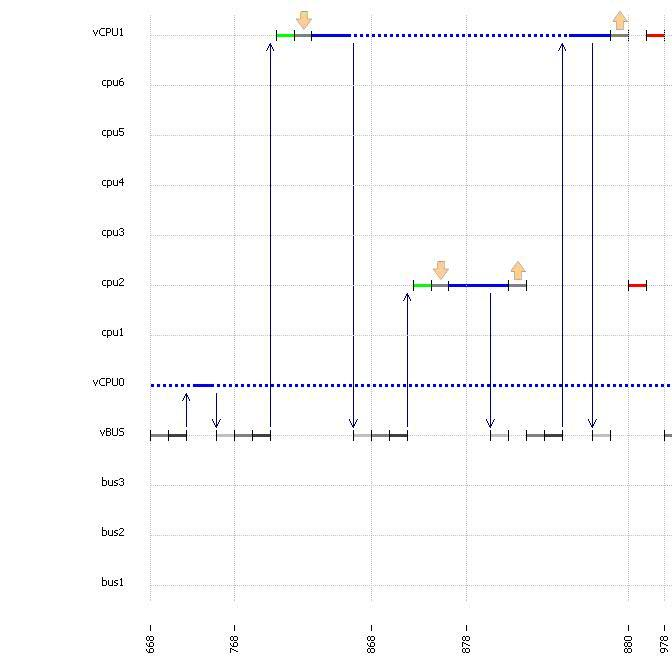
\includegraphics[width=\textwidth]{exeoverview}
\end{center}
\caption{防御対策例題のための実行概観からの抽出\label{fig:exeoverview}}
\end{figure}

\begin{figure}
\begin{center}
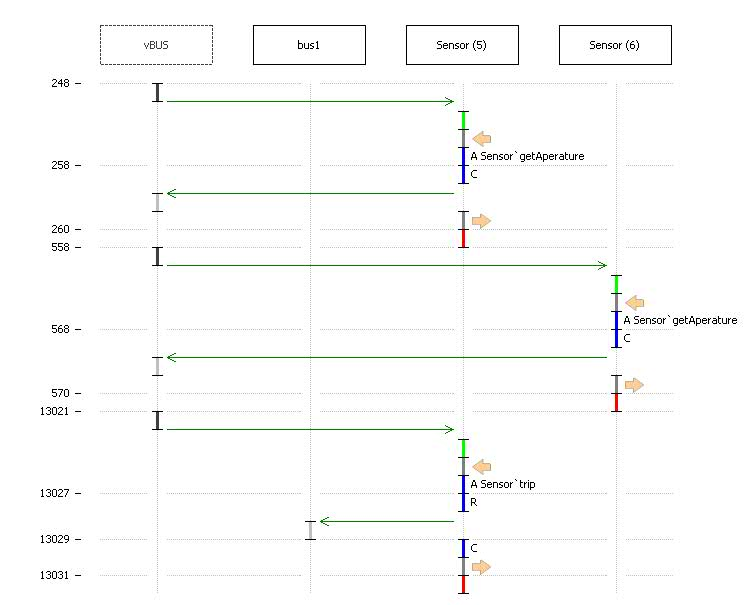
\includegraphics[width=\textwidth]{detailedexe}
\end{center}
\caption{防御対策例題のための1つの \texttt{CPU} 実行からの抽出\label{fig:detailedexe}}
\end{figure}

\subsection{注文仕立ての分析ツール}

もちろんたくさんの注文仕立ての分析ツールがあり、アプリケーションドメインや興味のあるリアルタイムプロパティに従って、トレースファイルのために配置も可能である。
ここで一般的なアプローチのいくつかに焦点をあてる。

\subsubsection{標準的テキスト処理ツールの使用}

タイムトレースファイルは単純な ASCII ファイルなので、このようなファイルの操作は直接的である (e.g.\ in Perl \cite{Wall&92}). 
この例としてPerlスクリプトがあるが、図~\ref{fig:chartExcel}で示される防御対策モデルの初期版より求まるトレースファイルから、Excelのスプレッドシートを生成するために用いられる。
この図式に、モデル中の多様なスレッドが作動する時刻の画像描写が見れる。
標準のオフィスツールでコンマ区切りのファイルを受け取ることができるので、このようなスクリプトを書くことがそのまま連続データを処理することである。

\subsubsection{視覚化}

共通する注文仕立ての分析ツールはトレースの視覚化であり、そこに時刻を載せることで特定の事象がスレッドのアクティビティライン上で起きる。
この例題は図~\ref{fig:vistrace}に示されている。

 Java Swing\cite{JavaSwing}、Qt \cite{Qt}、Visual Basic \cite{VisualBasic}といった圧倒的多数のGUIツールキットが与えられて、 このような視覚化は比較的開発しやすい、しかし \texttt{showtrace}ツールを用いるよりも確かに多くの時間を費やす。
さらにモデル動作を交信することはかなり力強いことであり得る。

\begin{figure}
\begin{center}
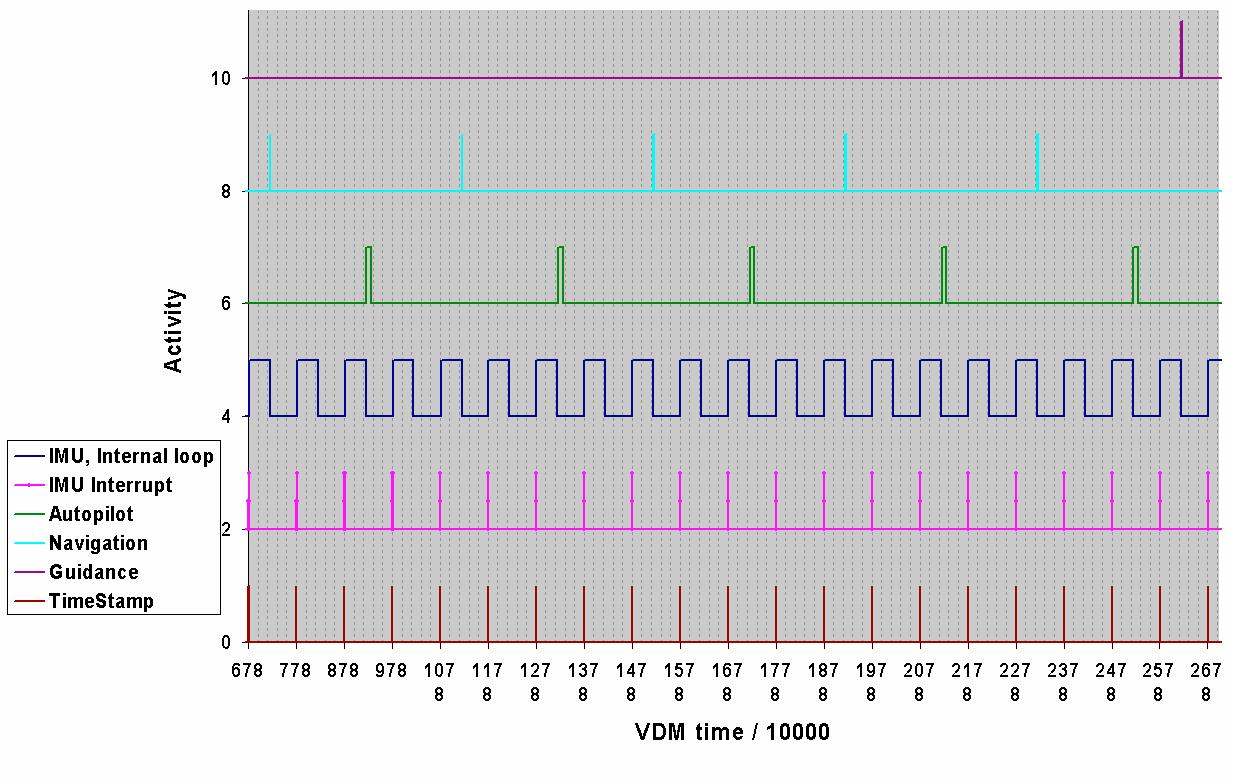
\includegraphics[width=\textwidth]{analysismissile}
\end{center}
\caption{タイムトレースファイルから生成した Microsoft Excel チャート\label{fig:chartExcel}}
\end{figure}

\begin{figure}
\begin{center}
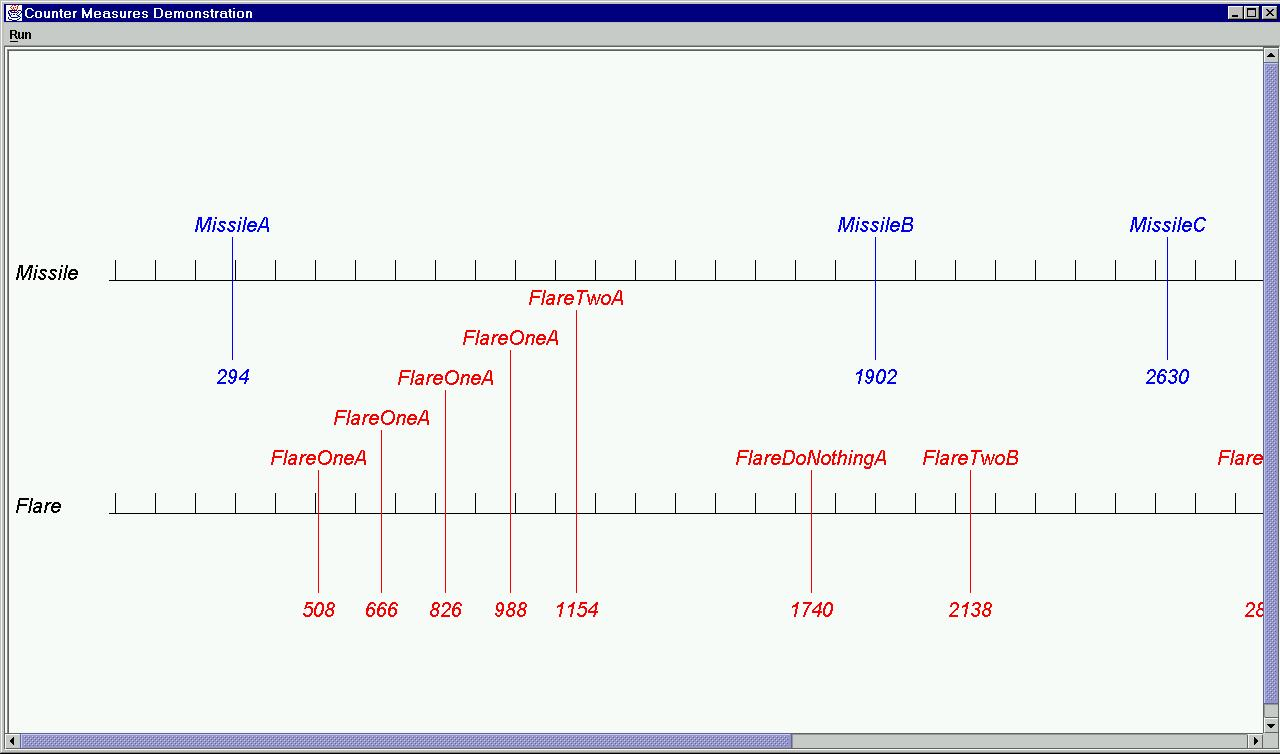
\includegraphics[width=\textwidth]{bespokemissile}
\end{center}
\caption{タイムトレースファイルの視覚化\label{fig:vistrace}}
\end{figure}

\subsubsection{タイムスタンプ表明}

タイムトレースファイルは単純な一列と考えることができる。
したがって VDM-SL 述語をこのような一列上に指定することが可能だ。

これを可能とするために、トレースファイルの抽象的な VDM-SL 表現が必要である。
それがここに述べられている。

たくさんの型が様々な分野を1つのタイムトレースファイルに表現するために、定義されている。
文字の列として文字列を、自然数としてオブジェクト参照とスレッドidsを、表現する。

\begin{lstlisting}
types

  String = seq of char;
  OBJ_Ref = nat;
  ThreadId = nat;
\end{lstlisting}

トレースはトレース事象の順付け列である。

\begin{lstlisting}
Trace = seq of TraceEvent
\end{lstlisting}

たくさんの様々な種類のトレース事象がある。

\begin{lstlisting}
TraceEvent = 
     ThreadSwapIn | ThreadSwapOut | DelayedThreadSwapIn |
     OpRequest | OpActivate | OpCompleted | ThreadCreate |
     ThreadKill |  MessageRequest | MessageActivate |
     MessageCompleted | ReplyRequest | CPUdecl | BUSdecl |
     DeployObj; 
\end{lstlisting}

事象におけるスレッド交換は、スワップインされるスレッドのid、スレッドを所有しているオブジェクト参照、そこでスレッドが定義されたクラス名、実行場所の cpu 、スレッドにおけるスワップの超過時間、その \texttt{CPU}上の時間、からなる。

\begin{lstlisting}
  ThreadSwapIn :: id       : ThreadId
                  objref   : [OBJ_Ref]
                  clnm     : String
                  cpunm    : nat 
                  overhead : nat
                  time     : nat;
\end{lstlisting}

遅滞スレッドのスワップインは遅滞を表わす余分な項目をもつ。

\begin{lstlisting}
DelayedThreadSwapIn :: id       : ThreadId
                       objref   : [OBJ_Ref]
                       clnm     : String
                       delay    : real
                       cpunm    : nat
                       overhead : nat
                       time     : nat;
\end{lstlisting}

スレッドのスワップアウトは、スレッドのスワップインと同じ情報を含む。

\begin{lstlisting}
ThreadSwapOut :: id       : ThreadId
                 objref   : [OBJ_Ref]
                 clnm     : String
                 cpunm    : nat
                 overhead : nat
                 time     : nat;
\end{lstlisting}

操作要求には、要求が成されたスレッド、操作の名称、要求が発生したオブジェクトに対する参照、このオブジェクトがインスタンスであるクラスの名称、実行中の cpu 、(もし特別なユーザーオプションがこの情報の詳細レベルの保存に対し設定されているならば)それらの操作の引数、最後にそれが非同期の操作であろうとなかろうとその \texttt{CPU}上の時刻、が含まれる。

\begin{lstlisting}
OpRequest :: id     : ThreadId
             opname : String
             objref : OBJ_Ref
             clnm   : String
             cpunm  : nat
             args   : [seq of VAL]
             async  : bool
             time   : nat;
\end{lstlisting}

操作の発動と完了では、操作要求としての情報の一部が含まれる(操作の結果は、ユーザーが明示的にこの情報のログを頼んでいた場合のみ存在するが)。

\begin{lstlisting}
OpActivate :: id     : ThreadId
              opname : String
              objref : OBJ_Ref
              clnm   : String
              cpunm  : nat
              async  : bool
              time   : nat;

OpCompleted :: id     : ThreadId
               opname : String
               objref : OBJ_Ref
               clnm   : String
               cpunm  : nat
               res    : [VAL]
               async  : bool
               time   : nat;
\end{lstlisting}

トレース事象はまた、スレッドの生成中と完了後の抹殺中には常に存在している。
スレッドの生成中は、それが周期的スレッドであるかどうかの情報も含むことに注意しよう。

\begin{lstlisting}
ThreadCreate :: id     : ThreadId
                period : bool
                objref : [OBJ_Ref]
                clnm   : [String] 
                cpunm  : nat
                time   : nat;

ThreadKill :: id    : ThreadId
              cpunm : nat
              time  : nat;
\end{lstlisting}

様々な\texttt{CPU}の間でメッセージがやり取りされるとき、たくさんの事象が現れる。操作に関しても、同様の要求、起動、完了の枠組みに従う。
しかしながら、同期の操作に対しては特別な応答要求メッセージ事象があり、様々な \texttt{CPU} 上の操作の実行結果を正しい \texttt{CPU} と同様にその正しいスレッドに導いていくことに用いられる。
それ以外では、以下で用いられている項目はむしろ自明であろう。

\begin{lstlisting}
MessageRequest ::
  busid   : nat
  fromcpu : nat
  tocpu   : nat
  msgid   : nat
  callthr : ThreadId
  opname  : String
  objref  : [OBJ_Ref]
  size    : nat
  time    : nat;

ReplyRequest ::
  busid     : nat
  fromcpu   : nat
  tocpu     : nat
  msgid     : nat
  origmsgid : nat
  callthr   : ThreadId
  calleethr : ThreadId
  size      : nat
  time      : nat;

MessageActivate ::
  msgid : nat
  time  : nat;

MessageCompleted ::
  msgid : nat
  time  : nat;
\end{lstlisting}

\texttt{CPU}と \texttt{BUS}の宣言もまた、システム構造の全体を描くことができるように、トレースファイルにログが記録される。

\begin{lstlisting}
CPUdecl ::
  id   : nat
  name : String
  expl : bool;
  
BUSdecl ::
  id   : nat
  topo : set of nat
  name : String;

DeployObj ::
  objref : OBJ_Ref
  cpunm  : nat
  time   : nat
\end{lstlisting}
 
これは、トレースファイルの表示に必要な型の定義を決定することとなる。

タイムスタンプ表明を描くために、いくつかの例を挙げる。
簡単な表明としては、遅滞するスレッドはいずれも、いくらかの目的とする最高限度内での遅滞をもつ、ということである。
これは関数\texttt{MaximumDelay}で表現されている。

\begin{lstlisting}
functions

MaximumDelay: real * Trace -> bool
MaximumDelay(maxDelay, trace) ==
  forall ti in set elems trace &
     is_DelayedThreadSwapIn(ti) => ti.delay <= maxDelay;
\end{lstlisting}

もう少し複雑な表明では実行されるべき操作に対してとられる時間に関連する。
特別な操作がいつ発動されるときはいつも、関数 \texttt{MaximumOpExecutionTime}を用いて指定の期間内に実行を完了する、ということを指定することができる。

\begin{lstlisting}
MaximumOpExecutionTime: String * real * Trace -> bool
MaximumOpExecutionTime(opname, maxExecTime, trace) ==
  forall i in set inds trace &
     is_OpActivate(trace(i)) =>
        trace(i).opname = opname =>
           let opcompleteIndex = NextOpComplete(opname, i,
                                                trace) in
             trace(opcompleteIndex).time - trace(i).time <= 
             maxExecTime;
\end{lstlisting}

\texttt{MaximumOpExecutionTime}は 補助関数\texttt{NextOpComplete}を用いる。 
これは 索引\texttt{i}で発動される操作起動に対して、相当する操作完了の索引を見つける。

\begin{lstlisting}
NextOpComplete: String * nat * Trace -> nat
NextOpComplete(opname, i, trace) ==
  hd [ j | j in set inds trace
         & j > i and
           is_OpCompleted(trace(j)) and 
           trace(j).opname = opname]
pre exists j in set inds trace & 
       is_OpCompleted(trace(j)) and
       j > i and trace(j).opname = opname
\end{lstlisting}

何れかの段階でこの種のタイムスタンプ表明分析が\texttt{showtrace} といった一般的なツールに、あるいはたぶん将来は \vdmtools\ 内に直接、組み込める、を想することもまた可能である。

\section{調整}

タイムトレースファイルの分析では、事象が起きる時刻の翻訳を含んでいる。
本書で記述されているアプローチにしたがえば、これらの時刻は、時間が対象プロセッサ上で対象のリアルタイムカーネルを用いて進行していくという方法のシミュレーションである。
対象マシンがシミュレートされた時刻に作用するこの方法は、既定時刻の使用によるものであり、これは対象プロセッサ上のアセンブり命令を実行するために取られた時刻に相当する。

しかし、これは近似である、なぜなら VDM++ インタープリタは独自の命令集合をもち、どのようなプロセッサのものとも一致しないであろうからだ。
したがって不可避的に既定時刻との調整要素が生まれ、シミュレーションの精度を改善するであろう。
この調整は \emph{calibration}として参照される。.

通常は、対象上の実際のアプリケーション実行により得られたタイムトレースを、 VDM++ モデルを実行させることで得られたものとの比較して調整する。N VDM++ モデルは決定論的であるため、実際のアプリケーションに合致させていくために、様々な既定時刻の集合ではなく1つのシナリオでもって再実行が可能である。
自然なアプローチとしては、シミュレーションは実際のアプリケーションのタイミング動作に厳密に一致させることはできないということ; 求められる性質は、アプリケーションがタイミング上のボトルネックを示すことがないということで、 VDM++ モデルではボトルネックは確認されていない。

\chapter{追記}\label{chap:postscript}

本書では、 \VDMTools を用いてどのように応答リアルタイム分散システムを開発することができるかを述べてきた。
どのように応答リアルタイムシステムの主要な特徴が \VDMTools を用いることでモデル化され分析できるかに、焦点を当ててきた。
これは便利な開発アプローチに向けて1つの発展性ある選択肢である、というのが一番のメッセージである。
初期フェーズにはさらに多くの時間が費やされるが、様々な設計における従来より早く必要なタイミング要求と出会う力から、更なる確信が得られている。
主要な疑問として挙げられるのが、初期フェーズにおける投資は価値があるのかということである。
特に最終的なハードウェアプラットフォームに対するアクセスが制限されているとか、まったくまだ決定されていないといった状況において、このことが正当と見なされると感じている。
しかし、ここで提示したアプローチが正しいシステムを常に保証する魔法の処方箋であると主張したいわけではない。
ここで述べてきたアプローチは従来の開発アプローチよりさらに厳格なものである、ということを単に提示することを望むもので、またこれは正しい方向に向けての実際的な一歩であると感じている。

%\chapter{References}

\bibliographystyle{iptes}
\bibliography{dan}

\newpage
\appendix

\chapter{用語解説}\label{app:glossary}

\begin{description}
\item[遮断された] スレッドの状態で、許可述語が真となるのを待っていて処理を進めることができない。
\item[ボトルネック] システムの一部で、このタイミング動作が決定的にシステム全体の性能に影響を与える。
\item[並列実時間分散 VDM++ 設計モデル] 特定の動的および物理的構造を定義するモデルであり、そのリアルタイム動作と複数 \texttt{CPU}に対する展開を含める。
\item[並列 VDM++ 設計モデル] 特定の動的構造を定義するモデルであり、最初のインスタンスにおいてはリアルタイム動作は考慮しない
\item[既定継続情報] 写像であり、対象プロセッサ上のアセンブリ命令の実行回数を記録する。
\item[既定スレッド] スレッドであり、モデルの実行を初期化する。
ユーザーにより \vdmtools\ インタープリタにおいてスタートさせられるか、あるいはスクリプト中のコマンドによってスタートさせられる。
\item[動的構造] プロセス(スレッド)に対する計算結果の写像。
\item[厳しい期限(Hard Deadline)] システムが、何らかのアクションを完了しなければならない時点のこと; このような期限に対する失敗は許されていない。
\item[ジッター] 周期的事象が完全に周期的ではないというプロパティで、しかし期待される出来事が何らかの時間間隔内で起きる。
\item[スケジュール化可能] スレッドに対しては、 スレッドは既にスタートしていて、現在は実行中ではないが遮断もされていないことを意味する。
システムに対しては、期限をミスするスレッドもなくシステムが実行されることが可能であることを意味する。
\item[逐次 VDM++ 設計モデル] 特定の動的構造について取り上げることはせず、計算されるべきデータとどのようにそれを静的クラスに構造化するべきかを述べなければならない。
\item[穏やかな期限(Soft Deadline)] ある時点のことで、システムはその時点までに何らかのアクションを実行しなければならない; このようなデッドラインに対する時折の失敗は許されているが、失敗が繰り返される場合にはシステムの実効性低下を導くことになる。.
\item[静的構造] オブジェクトに対するシステム動作の取り決めである。
\item[タイムトレースファイル]  \vdmtools によるリアルタイムモデルの実行中に生成されるファイルで、モデルのランタイム動作についての情報を含んでいる。
\item[トレース事象] スワップインアウトが行われるスレッドの発生、あるいは操作の要求、発動、完了の発生のこと。
\item[ユースケース] これはシステムに見込まれる利用法である。
\item[VDM-SL システム仕様] これは詳細な抽象的設計から独立したシステム記述である。
\end{description}


\chapter{設計パターン}\label{app:patterns}

この章では、設計パターンをいくつか提示する。
これらは抽象的テクニックであり、多くのリアルタイムアプリケーション開発中に役に立つと取り上げられたものである。

\section{生データパターン}

生データパターンはデータアクセスの同期のためのパターンである。
ハードウェアデバイスがモデル化されたモデルで用いられるが、そのデバイスにより生成されたデータ値はもう1つのスレッドによって明記される。
生データパターンはその後3つのスレッド間の交信を仲介する:

\begin{description}
\item[インハビタ] -- 通常はハードウェアデバイスにより生成されるデータに相当するテストデータと共にモデルにおかれているスレッド。
\item[プロキシ] -- ハードウェアデバイスのモデルであるスレッド。
実際のハードウェアデバイスが提供するものに相当するインターフェイスとアクションを提供する。
\item[コンシューマ] -- ハードウェアデバイスにより生成されるデータを消費するスレッド。インハビタとプロキシ間の関係はコンシューマには見えない。
\end{description}

 図~\ref{fig:freshdata}に見られるパターン中のmainクラス同士の関係を示すダイアグラム。

 図~\ref{fig:seqdiafresh} に見られるシーケンス図がパターンからの抜粋を描いている。
パターンは \texttt{Inhabitor`Inhabit}の周期的実行に基づいている。
シーケンス図において、前述の期間に\texttt{Proxy`WaitFreshData}への呼び出しがある。
この呼び出しは遮断されている。
次の期間は \texttt{Inhabitor`Inhabit}への呼び出しで始まる。
これはデータを獲得するために順に独自の操作である \texttt{GetData} を呼び出し、このデータを \texttt{PutData} に送るために \texttt{Proxy}を呼ぶ。 
\texttt{PutData} の呼び出しは 遮断していた\texttt{WaitFreshData}への呼び出しを自由にする。

\begin{figure}
\begin{center}
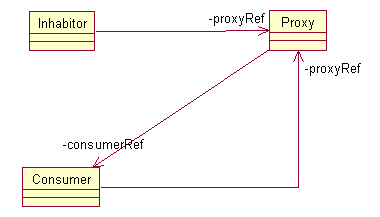
\includegraphics[width=0.5\textwidth]{freshdata}
\end{center}
\caption{生データパターンのためのクラス図\label{fig:freshdata}}
\end{figure}

 \texttt{Proxy} はその後 \texttt{Consumer} にデータが利用できることを伝えることができるが、 \texttt{Consumer}は余裕があるときにそれにアクセスできる。

\texttt{Data} クラスはそのパターン中で用いられたデータ値を表すのに用いられる。
このようにこれはまさに場所確保でありしたがってこの場合には内容はない。

\begin{lstlisting}
class Data
end Data
\end{lstlisting}

\subsection{インハビタ}

 \texttt{Inhabitor} クラスはテスト目的のデータをモデルにおくために用いられる。
このデータを \texttt{Proxy}中におくが、それに対する参照を持つ。
この参照はインスタンス変数として保存される。

\begin{lstlisting}
class Inhabitor

instance variables
  proxyRef : Proxy
\end{lstlisting}

\texttt{Proxy}に対する参照を初期化するために、コンシューマが用いられる。

\begin{lstlisting}
operations
  public Inhabitor : Proxy ==> Inhabitor
  Inhabitor (proxy) ==
    proxyRef := proxy;
\end{lstlisting}

\begin{figure}
\begin{center}
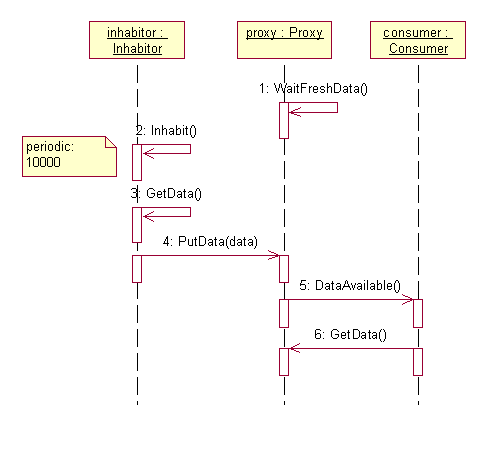
\includegraphics[width=\textwidth]{freshdataseqdiag}
\end{center}
\caption{生データパターンのためのシーケンス図\label{fig:seqdiafresh} }
\end{figure}

データは \texttt{Inhabit} 操作を用いてプロキシへ送られる。

\begin{lstlisting}
Inhabit : () ==> ()
Inhabit() ==
  proxyRef.PutData(GetData());
\end{lstlisting}

操作 \texttt{GetData} は実際にデータ値を獲得するために用いられる。
ここで指定されないで残ったのが; モデルにおいてデータをファイルから読むかもしれないということ。

\begin{lstlisting}
GetData : () ==> Data
GetData() ==
  is not yet specified
\end{lstlisting}

 \texttt{Inhabitor} スレッドは一定期間 \texttt{Inhabit} 操作を呼び出すが、ここで任意に 10000 になるまで選択されるが、ジッターと共に100時間単位、最小遅滞は9900時間単位が最低限の。

\begin{lstlisting}
thread
  periodic (10000,100,9900,0)(Inhabit)

end Inhabitor
\end{lstlisting}

\subsection{プロキシ}

 \texttt{Proxy} クラスは同じインターフェイスを提供し、実際のデバイスを意図した、しかしデバイスが \texttt{Inhabitor}から生成するデータを取る.

これは3つのインスタンス変数をもつ:

\begin{description}
\item[\texttt{d}] 最も最近に生成されたデータ値、あるいは生データが存在しなければ \texttt{nil}。
\item[\texttt{freshData}] 生データが存在するかどうかを示すブール値。
\item[\texttt{consumerRef}]  \texttt{Consumer}への参照。
\end{description}

\begin{lstlisting}
class Proxy

instance variables
  d : [Data] := nil;
  freshData : bool := false;
  consumerRef : Consumer
\end{lstlisting}

構成子は \texttt{Consumer} 参照を初期化するために用いられる。

\begin{lstlisting}
operations

public Proxy : Consumer ==> Proxy
Proxy(consumer) ==
  consumerRef := consumer;
\end{lstlisting}

\texttt{PutData} は \texttt{Inhabitor} によりデータを\texttt{Proxy}へ送るために用いられる。

\begin{lstlisting}
public PutData : Data ==> ()
PutData(newData) ==
  ( d := newData;
    freshData := true
  );
\end{lstlisting}

\texttt{GetData} は \texttt{Consumer} により \texttt{Proxy}から生データを取り戻すために用いられる。

\begin{lstlisting}
public GetData : () ==> Data
GetData() ==
  let od = d in
  ( d := nil;
    return od
  );
\end{lstlisting}

\texttt{WaitFreshData} はこのクラスのスレッドにより生データが利用できるまで待つために用いられる。

\begin{lstlisting}
WaitFreshData : () ==> ()
WaitFreshData() ==
  freshData := false;

sync
  per WaitFreshData => freshData
\end{lstlisting}

このクラスに対するスレッドは繰り返し生データを待ちそしてコンシューマへその到着を知らせる。

\begin{lstlisting}
thread

while true do
( WaitFreshData();
  consumerRef.DataAvailable()
)

end Proxy
\end{lstlisting}

\subsection{コンシューマ}

コンシューマはシステムの残りに対するインターフェイスを表す。
 \texttt{Proxy} からデータ値を取りそれらが適していることが分かるように用いる。

3つのインスタンス変数が定義されている:

\begin{description}
\item[\texttt{dataAvailable}] 生データが利用できるか否かを示すブール値。
\item[\texttt{proxyRef}]  \texttt{Proxy}への参照で、データを取り戻すのに用いられる。
\item[\texttt{d}]  \texttt{Proxy}から取り戻したデータ値。
\end{description}

\begin{lstlisting}
class Consumer

instance variables
  dataAvailable : bool := false;
  proxyRef : Proxy;
  d : Data
\end{lstlisting}

構成子が \texttt{Proxy}への参照を初期化するのに用いられる。

\begin{lstlisting}
operations
  public Consumer : Proxy ==> Consumer
  Consumer(proxy) ==
    proxyRef := proxy;
\end{lstlisting}

\texttt{DataAvailable} が生データの到着を示すために \texttt{Proxy} により用いられる。

\begin{lstlisting}
  public DataAvailable : () ==> ()
  DataAvailable() ==
    dataAvailable := true;
\end{lstlisting}

\texttt{GetData} はプロキシから生データを獲得するために用いられる。
生データが利用できない場合は常に遮断する。

\begin{lstlisting}
  GetData : () ==> ()
  GetData() ==
    (d := proxyRef.GetData();
     dataAvailable := false
    );

sync
  per GetData => dataAvailable
\end{lstlisting}

このクラスに対するスレッドは、データが利用できるときには繰り返しデータを取る。

\begin{lstlisting}
thread

  while true do
    GetData()

end Consumer
\end{lstlisting}

\section{タイムスタンプパターン}\label{sec:TimeStamp}

タイムスタンプパターンは同期システムで用いるものであり、各々の異なるスレッドは独自の実行期間をもつ。
このようなスレッドをクライアントとして参照する。
タイムスタンプパターンの main クラスは\texttt{TimeStamp} クラスで、これは 第~\ref{sec:waitnotify}章で述べた \texttt{WaitNotify}クラスの拡張である。
\texttt{TimeStamp} クラスの単一インスタンスは様々なクライアントすべての中で共有され、各クライアントがその実行期間のために起こされていることを保証するために用いられる。
描画目的で2つのクライアントクラスをもつ図~\ref{fig:classtimestamp} で例題配置が見れる。

サンプル実行は 図~\ref{fig:seqdiagtimestamp}に見られる。 
この例題中では3クライアント設定されていて: 2つの ``fast'' クライアントと1つの``slow'' クライアントである。
2つの fast クライアントはそれぞれが10 時間単位毎に実行期間をもち、一方の slow クライアントは30 時間単位毎の実行期間をもつ。
各クライアントはその実行期間と共に \texttt{TimeStamp`WaitRelative}を呼び出し、その時刻にあるいはその後すぐに起こされる。
起こされたときは各々のクライアントはその\texttt{ComputationPhase} -- 定期的に実行するように意図された計算 -- を実行する。
その \texttt{ComputationPhase} を実行するときには、待機中のクライアントを自由にするために\texttt{TimeStamp`Notify} を呼び出す。
クライアントはパターンに対しては偶然にあたるものであるから、以下の仕様にはあたらないことに注意しよう。

\subsection{タイムスタンプクラス}

 \texttt{TimeStamp} クラスは \texttt{WaitNotify} クラスを拡張する。
いつ特定のスレッドが起こされるべきかを表すことで、スレッドids から時刻への写像 (\texttt{wakeUpMap})を保持する。
したがって、この写像が正しく保持されることを確実にするため、 \texttt{WaitNotify} インターフェイスに優先する。
このクラスの他のインスタンス変数は現時刻を表す。
この概念は本書において先に述べたシミュレートされた時刻の概念に直交するものであることに注意しよう。

\begin{figure}
\begin{center}
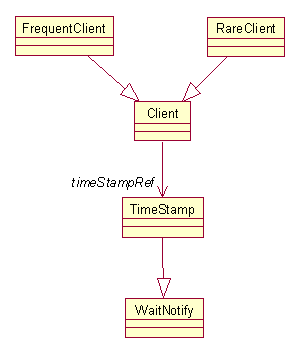
\includegraphics[width=0.5\textwidth]{timestamp}
\end{center}
\caption{タイムスタンプパターンのためのクラス図\label{fig:classtimestamp}}
\end{figure}

\begin{figure}
\begin{center}
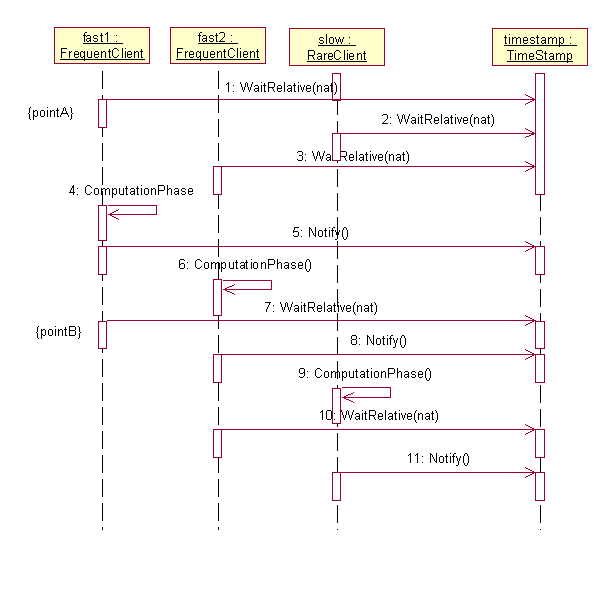
\includegraphics[width=\textwidth]{timestampseqdiag}
\end{center}
\caption{タイムスタンプパターンのためのシーケンス図\label{fig:seqdiagtimestamp}}
\end{figure}

\begin{lstlisting}
class TimeStamp is subclass of WaitNotify

instance variables
  
currentTime : nat := 0;
wakeUpMap : map nat to nat := {|->};
\end{lstlisting}

クライアントは相対的あるいは絶対的待機を要求してよい。
前者は \texttt{WaitRelative}を用いて実行される。

\begin{lstlisting}
operations

public WaitRelative : nat ==> ()
WaitRelative(val) ==
( AddToWakeUpMap(threadid, currentTime + val);
  WaitNotify`Wait();
);
\end{lstlisting}

絶対的待機は \texttt{WaitAbsolute}を用いて実行される。 
与えられた時刻が現時刻より小さいならば、クライアントが起こされることはないことに注意しよう。

\begin{lstlisting}
public WaitAbsolute : nat ==> ()
WaitAbsolute(val) ==
( AddToWakeUpMap(threadid, val);
  WaitNotify`Wait();
);
\end{lstlisting}

\texttt{AddToWakeUpMap} は \texttt{wakeUpMap}に対して新しい待機を追加するために用いられる。

\begin{lstlisting}
AddToWakeUpMap : nat * nat ==> ()
AddToWakeUpMap(tId, val) ==
  wakeUpMap := wakeUpMap ++ { tId |-> val };
\end{lstlisting}

以下の notify 操作は\texttt{WaitNotify} クラスのそれらに優先する。
特定のスレッドは \texttt{NotifyThread}を用いて早急に起こされ得る。

\begin{lstlisting}
public NotifyThread : nat ==> ()
NotifyThread(tId) ==
( wakeUpMap := {tId} <-: wakeUpMap;
  WaitNotify`NotifyThread(tId)
);
\end{lstlisting}

任意のスレッドは \texttt{Notify}を用いて早急に起こされる。

\begin{lstlisting}
public Notify : () ==> ()
Notify() ==
  let tId in set dom wakeUpMap in
    NotifyThread(tId);
\end{lstlisting}

すべての待機スレッドは\texttt{NotifyAll}を用いて早急に起こされる。

\begin{lstlisting}
public NotifyAll : () ==> ()
NotifyAll() ==
( wakeUpMap := {|->};
  WaitNotify`NotifyAll()
);
\end{lstlisting}

操作 \texttt{NotifyAndIncTime} は時刻を進め現時刻の進行を待つすべてのスレッドを起こすために用いられる。

\begin{lstlisting}
NotifyAndIncTime : () ==> ()
NotifyAndIncTime() ==
( currentTime := currentTime + 1;
  for all t in set dom (wakeUpMap :> {currentTime}) do
    NotifyThread(t)
);
\end{lstlisting}

そのクラスの現時刻は \texttt{GetTime}操作を経て得られる可能性がある。

\begin{lstlisting}
public GetTime : () ==> nat
GetTime() ==
  return currentTime;
\end{lstlisting}

\texttt{wakeUpMap} は多くの様々な操作により扱われているので、相互排除でいてそれらにアクセスを設定する必要がある。

\begin{lstlisting}
sync

  mutex(AddToWakeUpMap, Notify, NotifyThread, NotifyAll);
\end{lstlisting}

\chapter{Examples In Full}\label{app:listing}

\section{防御対策システムのための VDM-SLモデル}\label{app:VDMSLmodel}

\begin{lstlisting}
types

MissileInputs = seq of MissileInput;

MissileInput = MissileType * Angle;

MissileType = <MissileA> | <MissileB> | <MissileC> | <None>;

Angle = nat
inv num == num <= 360;

Output = map MagId to seq of OutputStep;

MagId = token;

OutputStep = FlareType * AbsTime;

Response = FlareType * Delay;

AbsTime = nat;

FlareType = <FlareOneA>  | <FlareTwoA>  | <FlareOneB> |
            <FlareTwoB>  | <FlareOneC>  | <FlareTwoC> |
            <DoNothingA> | <DoNothingB> | <DoNothingC>;

Plan = seq of (FlareType * Delay);

Delay = nat;

values

responseDB : map MissileType to Plan =
  {<MissileA> |-> [mk_(<FlareOneA>,900), mk_(<FlareTwoA>,500),
                   mk_(<DoNothingA>,100), mk_(<FlareOneA>,500)],
   <MissileB> |-> [mk_(<FlareTwoB>,500), mk_(<FlareTwoB>,700)],
   <MissileC> |-> [mk_(<FlareOneC>,400), mk_(<DoNothingC>,100),
                   mk_(<FlareTwoC>,400), mk_(<FlareOneC>,500)]
  };

missilePriority : map MissileType to nat
                = {<MissileA> |-> 1,
                   <MissileB> |-> 2,
                   <MissileC> |-> 3,
                   <None>     |-> 0};

stepLength : nat = 100;

testval1 : MissileInputs = [mk_(<MissileA>,88),
                            mk_(<MissileB>,70),
                            mk_(<MissileA>,222),
                            mk_(<MissileC>,44)];

testval2 : MissileInputs = [mk_(<MissileC>,188),
                            mk_(<MissileB>,70),
                            mk_(<MissileA>,2),
                            mk_(<MissileC>,44)];

testval3 : MissileInputs = [mk_(<MissileA>,288),
                            mk_(<MissileB>,170),
                            mk_(<MissileA>,222),
                            mk_(<MissileC>,44)];

functions

CounterMeasures: MissileInputs -> Output
CounterMeasures(missileInputs) ==
  CM(missileInputs,{|->},{|->},0);

CM: MissileInputs * Output * map MagId to [MissileType] * 
    nat -> Output
CM( missileInputs, outputSoFar, lastMissile, curTime) ==
  if missileInputs = []
  then outputSoFar
  else let mk_(curMis,angle) = hd missileInputs,
           magid = Angle2MagId(angle)
       in
         if magid not in set dom lastMissile or
            (magid in set dom lastMissile and
             missilePriority(curMis) > 
             missilePriority(lastMissile(magid)))
         then let newOutput = 
                     InterruptPlan(curTime,outputSoFar,
                                   responseDB(curMis),
                                   magid)
              in CM(tl missileInputs, newOutput, 
                    lastMissile ++ {magid |-> curMis},
                    curTime + stepLength)
         else CM(tl missileInputs, outputSoFar, 
                 lastMissile,curTime + stepLength);

InterruptPlan: nat * Output * Plan * MagId -> Output
InterruptPlan(curTime,expOutput,plan,magid) ==
  {magid |-> (if magid in set dom expOutput
              then LeavePrefixUnchanged(expOutput(magid), 
                                        curTime)
              else []) ^
              MakeOutputFromPlan(curTime, plan)} 
  munion
  ({magid} <-: expOutput);

LeavePrefixUnchanged: seq of OutputStep * nat -> 
                      seq of OutputStep
LeavePrefixUnchanged(output_l, curTime) ==
  [output_l(i) | i in set inds output_l
               & let mk_(-,t) = output_l(i) in t <= curTime];

MakeOutputFromPlan : nat * seq of Response -> seq of OutputStep
MakeOutputFromPlan(curTime, response) ==
  let output = OutputAtTimeZero(response) in
    [let mk_(flare,t) = output(i)
     in
       mk_(flare,t+curTime)
    | i in set inds output];

OutputAtTimeZero : seq of Response -> seq of OutputStep
OutputAtTimeZero(response) ==
  let absTimes = RelativeToAbsoluteTimes(response) in
    let mk_(firstFlare,-) = hd absTimes in
      [mk_(firstFlare,0)] ^
      [ let mk_(-,t) = absTimes(i-1),
            mk_(f,-) = absTimes(i) in
          mk_(f,t) | i in set {2,...,len absTimes}];

RelativeToAbsoluteTimes : seq of Response -> 
                          seq of (FlareType * Delay)
RelativeToAbsoluteTimes(ts) ==
  if ts = []
  then []
  else let mk_(f,t) = hd ts,
           ns = RelativeToAbsoluteTimes(tl ts) in
         [mk_(f,t)] ^ [ let mk_(nf, nt) = ns(i)
                        in mk_(nf, nt + t)
                      | i in set inds ns];

Angle2MagId: Angle -> MagId
Angle2MagId(angle) ==
  if angle < 90
  then mk_token("Magazine 1")
  elseif angle < 180
  then mk_token("Magazine 2")
  elseif angle < 270
  then mk_token("Magazine 3")
  else mk_token("Magazine 4");
\end{lstlisting}

\section{防御対策システムのための逐次VDM++モデル}

\subsection{CM クラス}

\begin{lstlisting}
class CM

instance variables

-- maintain a link to the detector
public static 
detector : MissileDetector := new MissileDetector();

public static sensor0 : Sensor := new Sensor(detector,0);
public static sensor1 : Sensor := new Sensor(detector,90);
public static sensor2 : Sensor := new Sensor(detector,180);
public static sensor3 : Sensor := new Sensor(detector,270);

public static 
controller0 : FlareController := new FlareController(0);
public static 
controller1 : FlareController := new FlareController(120);
public static 
controller2 : FlareController := new FlareController(240);

public static 
dispenser0 : FlareDispenser := new FlareDispenser(0);
public static 
dispenser1 : FlareDispenser := new FlareDispenser(30);
public static 
dispenser2 : FlareDispenser := new FlareDispenser(60);
public static 
dispenser3 : FlareDispenser := new FlareDispenser(90);

public static 
dispenser4 : FlareDispenser := new FlareDispenser(0);
public static 
dispenser5 : FlareDispenser := new FlareDispenser(30);
public static 
dispenser6 : FlareDispenser := new FlareDispenser(60);
public static 
dispenser7 : FlareDispenser := new FlareDispenser(90);

public static 
dispenser8 : FlareDispenser := new FlareDispenser(0);
public static 
dispenser9 : FlareDispenser := new FlareDispenser(30);
public static 
dispenser10 : FlareDispenser := new FlareDispenser(60);
public static 
dispenser11 : FlareDispenser := new FlareDispenser(90);

end CM
\end{lstlisting}

\subsection{World クラス}

\begin{lstlisting}
class World

instance variables
  
-- maintain a link to the environment
public static env : [Environment] := nil;
public static timerRef : Timer := new Timer();

operations

public World: () ==> World
World () ==
  (-- set-up the sensors
   env := new Environment("scenario.txt");
   env.addSensor(CM`sensor0);
   env.addSensor(CM`sensor1);
   env.addSensor(CM`sensor2);
   env.addSensor(CM`sensor3);

   -- add the first controller with four dispensers
   CM`controller0.addDispenser(CM`dispenser0);
   CM`controller0.addDispenser(CM`dispenser1);
   CM`controller0.addDispenser(CM`dispenser2);
   CM`controller0.addDispenser(CM`dispenser3);
   CM`detector.addController(CM`controller0);

   -- add the second controller with four dispensers
   CM`controller1.addDispenser(CM`dispenser4);
   CM`controller1.addDispenser(CM`dispenser5);
   CM`controller1.addDispenser(CM`dispenser6);
   CM`controller1.addDispenser(CM`dispenser7);
   CM`detector.addController(CM`controller1);
 
   -- add the third controller with four dispensers
   CM`controller2.addDispenser(CM`dispenser8);
   CM`controller2.addDispenser(CM`dispenser9);
   CM`controller2.addDispenser(CM`dispenser10);
   CM`controller2.addDispenser(CM`dispenser11);
   CM`detector.addController(CM`controller2);
  );

-- the run function blocks the user-interface thread
-- until all missiles in the file have been processed
public Run: () ==> ()
Run () == 
  env.Run()

end World
\end{lstlisting}

\subsection{Global クラス}

\begin{lstlisting}
class GLOBAL

values

public SENSOR_APERTURE = 90;
public FLARE_APERTURE = 120;
public DISPENSER_APERTURE = 30

types

-- there are three different types of missiles
public 
MissileType = <MissileA> | <MissileB> | <MissileC> | <None>;

-- there are nine different flare types, three per missile
public FlareType =
    <FlareOneA> | <FlareTwoA> | <DoNothingA> | 
    <FlareOneB> | <FlareTwoB> | <DoNothingB> | 
    <FlareOneC> | <FlareTwoC> | <DoNothingC>;

-- the angle at which the missile is incoming
public Angle = nat
inv num == num <= 360;

public EventId = nat

operations

public canObserve: Angle * Angle * Angle ==> bool
canObserve (pangle, pleft, psize) ==
  def pright = (pleft + psize) mod 360 in
    if pright < pleft
    -- check between [0,pright> and [pleft,360>
    then return (pangle < pright or pangle >= pleft)
    -- check between [pleft, pright>
    else return (pangle >= pleft and pangle < pright);
       
public getAperture: () ==> Angle * Angle
getAperture () == is subclass responsibility;

end GLOBAL
\end{lstlisting}

\subsection{Environment クラス}

\begin{lstlisting}
class Environment is subclass of GLOBAL

types

public inline  = EventId * MissileType * Angle * nat;
public outline = EventId * FlareType * Angle * nat * nat;

instance variables

-- access to the VDMTools stdio
io : IO := new IO();

-- the input file to process
inlines : seq of inline := [];

-- the output file to print
outlines : seq of outline := [];

-- maintain a link to all sensors
ranges : map nat to (Angle * Angle) := {|->};
sensors : map nat to Sensor := {|->};
inv dom ranges = dom sensors;

-- information about the latest event that has arrived
evid : [EventId] := nil;

busy : bool := true;

operations

public Environment: seq of char ==> Environment
Environment (fname) ==
  def mk_ (-,input) = io.freadval[seq of inline](fname) in
    inlines := input;

public addSensor: Sensor ==> ()
addSensor (psens) ==
  (dcl id : nat := card dom ranges + 1;
   atomic (
    ranges := ranges munion {id |-> psens.getAperture()};
    sensors := sensors munion {id |-> psens} 
   )
  );

public Run: () ==> ()
Run () == 
 (while not (isFinished() and 
        CM`detector.isFinished()) do
    (evid := createSignal();
     CM`detector.Step();
     World`timerRef.StepTime();
    );
 showResult()
 );

private createSignal: () ==> [EventId]
createSignal () ==
  (if len inlines > 0
   then (dcl curtime : nat := World`timerRef.GetTime(), 
             done : bool := false;
         while not done do
           def mk_ (eventid, pmt, pa, pt) = hd inlines in
             if pt <= curtime
             then (for all id in set dom ranges do
                     def mk_(papplhs,pappsize) = ranges(id) in
                       if canObserve(pa,papplhs,pappsize)
                       then sensors(id).trip(eventid,pmt,pa);
                   inlines := tl inlines;
                   done := len inlines = 0;
                   return eventid )
             else (done := true;
                   return nil ))
   else (busy := false;
         return nil));

public 
handleEvent: EventId * FlareType * Angle * nat * nat ==> ()
handleEvent (evid,pfltp,angle,pt1,pt2) ==
  (outlines := outlines ^ [mk_ (evid,pfltp, angle,pt1, pt2)] );

public showResult: () ==> ()
showResult () ==
  def - = io.writeval[seq of outline](outlines) in skip;

public isFinished : () ==> bool
isFinished () == 
  return inlines = [] and not busy;

end Environment
\end{lstlisting}

\subsection{Sensor クラス}

\begin{lstlisting}
class Sensor is subclass of GLOBAL

instance variables

-- the missile detector this sensor is connected to
private detector : MissileDetector;

-- the left hand-side of the viewing angle of the sensor
private aperture : Angle;

operations

public Sensor: MissileDetector * Angle ==> Sensor
Sensor (pmd, psa) == ( detector := pmd; aperture := psa);

-- get the left hand-side start point and opening angle
public getAperture: () ==> GLOBAL`Angle * GLOBAL`Angle
getAperture () == return mk_ (aperture, SENSOR_APERTURE);

-- trip is called asynchronously from the environment to
-- signal an event. the sensor triggers if the event is
-- in the field of view. the event is stored in the
-- missile detector for further processing
public trip: EventId * MissileType * Angle ==> ()
trip (evid, pmt, pa) ==
  -- log and time stamp the observed threat
  detector.addThreat(evid, pmt,pa,World`timerRef.GetTime())
pre canObserve(pa, aperture, SENSOR_APERTURE)

end Sensor
\end{lstlisting}

\subsection{MissileDetector クラス}

\begin{lstlisting}
class MissileDetector is subclass of GLOBAL

-- the primary task of the MissileDetector is to
-- collect all sensor data and dispatch each event
-- to the appropriate FlareController

instance variables

-- maintain a link to each controller
ranges : map nat to (Angle * Angle) := {|->};
controllers : map nat to FlareController := {|->};
inv dom ranges = dom controllers;

-- collects the observations from all attached sensors
threats : seq of (EventId * MissileType * Angle * nat) := [];

-- status of the missile detector
busy : bool := false

operations

-- addController is only used to instantiate the model
public addController: FlareController ==> ()
addController (pctrl) ==
  (dcl nid : nat := card dom ranges + 1;
   atomic
    (ranges := ranges munion {nid |-> pctrl.getAperture()};
     controllers := controllers munion {nid |-> pctrl}
    );
  );

public Step: () ==> ()
Step() ==
  (if threats <> []
   then def mk_ (evid,pmt, pa, pt) = getThreat() in
          for all id in set dom ranges do
            def mk_(papplhs, pappsize) = ranges(id) in
              if canObserve(pa, papplhs, pappsize)
              then controllers(id).addThreat(evid,pmt,pa,pt);
    busy := len threats > 0;
    for all id in set dom controllers do
      controllers(id).Step()
  );
 
-- addThreat is a helper operation to modify the event
-- list. currently events are stored first come first served.
-- one could imagine using a different ordering instead.
public addThreat: EventId * MissileType * Angle * nat ==> ()
addThreat (evid,pmt,pa,pt) == 
  (threats := threats ^ [mk_ (evid,pmt,pa,pt)];
   busy := true );

-- getThreat is a local helper operation to modify 
-- the event list
private getThreat: () ==> EventId * MissileType * Angle * nat
getThreat () ==
  (dcl res : EventId * MissileType * Angle * nat := hd threats;
   threats := tl threats;
   return res );

public isFinished: () ==> bool
isFinished () ==
  return forall id in set dom controllers &
            controllers(id).isFinished()

end MissileDetector
\end{lstlisting}

\subsection{FlareController クラス}

\begin{lstlisting}
class FlareController is subclass of GLOBAL

instance variables

-- the left hand-side of the working angle
private aperture : Angle;

-- maintain a link to each dispenser
ranges : map nat to (Angle * Angle) := {|->};
dispensers : map nat to FlareDispenser := {|->};
inv dom ranges = dom dispensers;

-- the relevant events to be treated by this controller
threats : seq of (EventId * MissileType * Angle * nat) := [];

-- the status of the controller
busy : bool := false

operations

public FlareController: Angle ==> FlareController
FlareController (papp) == aperture := papp;

public addDispenser: FlareDispenser ==> ()
addDispenser (pfldisp) ==
  let angle = aperture + pfldisp.GetAngle() in
    (dcl id : nat := card dom ranges + 1;
     atomic
     (ranges := ranges munion 
                {id |-> mk_(angle, DISPENSER_APERTURE)};
      dispensers := dispensers munion {id |-> pfldisp});
     );

public Step: () ==> ()
Step() ==
  (if threats <> []
   then def mk_ (evid,pmt, pa, pt) = getThreat() in
          for all id in set dom ranges do
            def mk_(papplhs, pappsize) = ranges(id) in
              if canObserve(pa, papplhs, pappsize)
              then dispensers(id).addThreat(evid,pmt,pt);
   busy := len threats > 0;
   for all id in set dom dispensers do
     dispensers(id).Step());
 
-- get the left hand-side start point and opening angle
public getAperture: () ==> GLOBAL`Angle * GLOBAL`Angle
getAperture () == return mk_(aperture, FLARE_APERTURE);

-- addThreat is a helper operation to modify the event
-- list. currently events are stored first come first served.
-- one could imagine using a different ordering instead
public addThreat: EventId * MissileType * Angle * nat ==> ()
addThreat (evid,pmt,pa,pt) ==
  (threats := threats ^ [mk_ (evid,pmt,pa,pt)];
   busy := true );

-- getThreat is a local helper operation to modify 
-- the event list
private getThreat: () ==> EventId * MissileType * Angle * nat
getThreat () ==
  (dcl res : EventId * MissileType * Angle * nat := hd threats;
   threats := tl threats;
   return res );

public isFinished: () ==> bool
isFinished () ==
  return forall id in set dom dispensers &
            dispensers(id).isFinished();

end FlareController
\end{lstlisting}

\subsection{FlareDispenser クラス}

\begin{lstlisting}
class FlareDispenser is subclass of GLOBAL

values

responseDB : map MissileType to Plan =
  {<MissileA> |-> [mk_(<FlareOneA>,900),
                   mk_(<FlareTwoA>,500),
                   mk_(<DoNothingA>,100),
                   mk_(<FlareOneA>,500)],
   <MissileB> |-> [mk_(<FlareTwoB>,500),
                   mk_(<FlareTwoB>,700)],
   <MissileC> |-> [mk_(<FlareOneC>,400),
                   mk_(<DoNothingC>,100),
                   mk_(<FlareTwoC>,400),
                   mk_(<FlareOneC>,500)] };

missilePriority : map MissileType to nat =
  {<None>     |-> 0,
   <MissileA> |-> 1,
   <MissileB> |-> 2,
   <MissileC> |-> 3 }

types

public Plan = seq of PlanStep;

public PlanStep = FlareType * Delay;

instance variables

public curplan : Plan := [];
curprio        : nat := 0;
busy           : bool := false;
aperture       : Angle;
eventid        : [EventId];

operations

public FlareDispenser: nat ==> FlareDispenser
FlareDispenser(ang) ==
  aperture := ang;
  
public Step: () ==> ()
Step() ==
  if len curplan > 0
  then (dcl curtime : nat := World`timerRef.GetTime(),
            first : PlanStep := hd curplan,
            next : Plan := tl curplan;
        let mk_(fltp, fltime) = first in
          (if fltime <= curtime
           then (releaseFlare(eventid,fltp,fltime,curtime);
                 curplan := next;
                 if len next = 0
                 then (curprio := 0; 
                       busy := false ) )
           )
    );

public GetAngle: () ==> nat
GetAngle() ==
  return aperture;

public addThreat: EventId * MissileType * nat ==> ()
addThreat (evid, pmt, ptime) ==
  if missilePriority(pmt) > curprio
  then (dcl newplan : Plan :=  [],
            newtime : nat := ptime;
        -- construct an absolute time plan
        for mk_(fltp, fltime) in responseDB(pmt) do
          (newplan := newplan ^ [mk_ (fltp, newtime)];
           newtime := newtime + fltime );
        -- immediately release the first action
        def mk_(fltp, fltime) = hd newplan;
            t = World`timerRef.GetTime() in
          releaseFlare(evid,fltp,fltime,t);
        -- store the rest of the plan
        curplan := tl newplan;
        eventid := evid;
        curprio := missilePriority(pmt);
        busy := true );

private releaseFlare: EventId * FlareType * nat * nat==> ()
releaseFlare (evid,pfltp, pt1, pt2) == 
  World`env.handleEvent(evid,pfltp,aperture,pt1,pt2);

public isFinished: () ==> bool
isFinished () == 
  return not busy

end FlareDispenser
\end{lstlisting}

\subsection{Timer クラス}\label{sec:timerapp}

\begin{lstlisting}
class Timer

instance variables

currentTime : nat := 0;

values

stepLength : nat = 10;

operations

public StepTime : () ==> ()
StepTime() ==
  currentTime := currentTime + stepLength;

public GetTime : () ==> nat
GetTime() ==
  return currentTime;

end Timer
\end{lstlisting}

\subsection{IO クラス}

\begin{lstlisting}
class IO

--  VDMTools STANDARD LIBRARY: INPUT/OUTPUT
--      --------------------------------------------
-- 
-- Standard library for the VDMTools Interpreter. When the 
-- interpreter evaluates the preliminary functions/operations 
-- in this file, corresponding internal functions is called 
-- instead of issuing a run time error. Signatures should not 
-- be changed, as well as name of module (VDM-SL) or class 
-- (VDM++). Pre/post conditions is fully user customisable. 
-- Dont care's may NOT be used in the parameter lists.
--
-- The in/out functions will return false if an error occurs. 
-- In this case an internal error string will be set 
-- (see 'ferror').

types
 
public
filedirective = <start>|<append> 

functions

-- Write VDM value in ASCII format to std out:
public
writeval[@p]: @p -> bool
writeval(val)==
  is not yet specified;

-- Write VDM value in ASCII format to file.
-- fdir = <start> will overwrite existing file,
-- fdir = <append> will append output to the file (created if
-- not existing).
public
fwriteval[@p]:seq1 of char * @p * filedirective -> bool
fwriteval(filename,val,fdir) ==
  is not yet specified;

-- Read VDM value in ASCII format from file
public
freadval[@p]:seq1 of char -> bool * [@p]
freadval(f) ==
  is not yet specified
  post let mk_(b,t) = RESULT in not b => t = nil;

operations

-- Write text to std out. Surrounding double quotes will be 
-- stripped, backslashed characters should be interpreted.
public
echo: seq of char ==> bool
echo(text) ==
  fecho ("",text,nil);

-- Write text to file like 'echo'
public
fecho: seq of char * seq of char * [filedirective] ==> bool
fecho (filename,text,fdir) ==
  is not yet specified
  pre filename = "" <=> fdir = nil;

-- The in/out functions  will return false if an error occur. 
-- In this case an internal error string will be set. 'ferror' 
-- returns this string and set it to "".
public
ferror:()  ==> seq of char
ferror () ==
  is not yet specified
end IO
\end{lstlisting}

\section{防御対策システムのための並列VDM++モデル}\label{app:concurCM}
\subsection{CM クラス}

\begin{lstlisting}
class CM

instance variables

-- maintain a link to the detector
public 
static detector : MissileDetector := new MissileDetector();

public static sensor0 : Sensor := new Sensor(detector,0);
public static sensor1 : Sensor := new Sensor(detector,90);
public static sensor2 : Sensor := new Sensor(detector,180);
public static sensor3 : Sensor := new Sensor(detector,270);

public static 
controller0 : FlareController := new FlareController(0);
public static 
controller1 : FlareController := new FlareController(120);
public static 
controller2 : FlareController := new FlareController(240);

public static 
dispenser0 : FlareDispenser := new FlareDispenser(0);
public static 
dispenser1 : FlareDispenser := new FlareDispenser(30);
public static 
dispenser2 : FlareDispenser := new FlareDispenser(60);
public static 
dispenser3 : FlareDispenser := new FlareDispenser(90);

public static 
dispenser4 : FlareDispenser := new FlareDispenser(0);
public static 
dispenser5 : FlareDispenser := new FlareDispenser(30);
public static 
dispenser6 : FlareDispenser := new FlareDispenser(60);
public static 
dispenser7 : FlareDispenser := new FlareDispenser(90);

public static 
dispenser8 : FlareDispenser := new FlareDispenser(0);
public static 
dispenser9 : FlareDispenser := new FlareDispenser(30);
public static 
dispenser10 : FlareDispenser := new FlareDispenser(60);
public static 
dispenser11 : FlareDispenser := new FlareDispenser(90);

end CM
\end{lstlisting}

\subsection{World クラス}

\begin{lstlisting}
class World

instance variables

-- maintain a link to the environment
public static env : [Environment] := nil;
public static timerRef : TimeStamp := new TimeStamp();

operations

public World: () ==> World
World () ==
  (-- set-up the sensors
   env := new Environment("scenario.txt");
   env.addSensor(CM`sensor0);
   env.addSensor(CM`sensor1);
   env.addSensor(CM`sensor2);
   env.addSensor(CM`sensor3);

   -- add the first controller with four dispensers
   CM`controller0.addDispenser(CM`dispenser0);
   CM`controller0.addDispenser(CM`dispenser1);
   CM`controller0.addDispenser(CM`dispenser2);
   CM`controller0.addDispenser(CM`dispenser3);
   CM`detector.addController(CM`controller0);

   -- add the second controller with four dispensers
   CM`controller1.addDispenser(CM`dispenser4);
   CM`controller1.addDispenser(CM`dispenser5);
   CM`controller1.addDispenser(CM`dispenser6);
   CM`controller1.addDispenser(CM`dispenser7);
   CM`detector.addController(CM`controller1);
 
   -- add the third controller with four dispensers
   CM`controller2.addDispenser(CM`dispenser8);
   CM`controller2.addDispenser(CM`dispenser9);
   CM`controller2.addDispenser(CM`dispenser10);
   CM`controller2.addDispenser(CM`dispenser11);
   CM`detector.addController(CM`controller2);
      
   -- start the detector
   start(CM`detector) );

-- the run function blocks the user-interface thread
-- until all missiles in the file have been processed
public Run: () ==> ()
Run () == 
  (-- start the environment
   start (env);
   -- wait for the environment to handle all input
   env.isFinished();
   -- wait for the missile detector to finish
   CM`detector.isFinished();
   -- print the result
   env.showResult())

end World
\end{lstlisting}

\subsection{Global クラス}

\begin{lstlisting}
class GLOBAL

values

public SENSOR_APERTURE = 90;
public FLARE_APERTURE = 120;
public DISPENSER_APERTURE = 30

types

-- there are three different types of missiles
public 
MissileType = <MissileA> | <MissileB> | <MissileC> | <None>;

-- there are nine different flare types, three per missile
public FlareType =
    <FlareOneA> | <FlareTwoA> | <DoNothingA> | 
    <FlareOneB> | <FlareTwoB> | <DoNothingB> | 
    <FlareOneC> | <FlareTwoC> | <DoNothingC>;

-- the angle at which the missile is incoming
public Angle = nat
inv num == num <= 360;

public EventId = nat

operations

public canObserve: Angle * Angle * Angle ==> bool
canObserve (pangle, pleft, psize) ==
  def pright = (pleft + psize) mod 360 in
    if pright < pleft
    -- check between [0,pright> and [pleft,360>
    then return (pangle < pright or pangle >= pleft)
    -- check between [pleft, pright>
    else return (pangle >= pleft and pangle < pright);
       
public getAperture: () ==> Angle * Angle
getAperture () == is subclass responsibility;

end GLOBAL
\end{lstlisting}

\subsection{Environment クラス}

\begin{lstlisting}
class Environment is subclass of GLOBAL

types

public inline  = EventId * MissileType * Angle * nat;
public outline = EventId * FlareType * Angle * nat * nat

instance variables

-- access to the VDMTools stdio
io : IO := new IO();

-- the input file to process
inlines : seq of inline := [];

-- the output file to print
outlines : seq of outline := [];

-- maintain a link to all sensors
ranges : map nat to (Angle * Angle) := {|->};
sensors : map nat to Sensor := {|->};
inv dom ranges = dom sensors;

-- information about the latest event that has arrived
evid : [EventId] := nil;

busy : bool := true;

operations

public Environment: seq of char ==> Environment
Environment (fname) ==
  def mk_ (-,input) = io.freadval[seq of inline](fname) in
    inlines := input;

public addSensor: Sensor ==> ()
addSensor (psens) ==
  (dcl id : nat := card dom ranges + 1;
   atomic (
    ranges := ranges munion {id |-> psens.getAperture()};
    sensors := sensors munion {id |-> psens} 
   )
  );

private createSignal: () ==> ()
createSignal () ==
  (if len inlines > 0
   then (dcl curtime : nat := World`timerRef.GetTime(), 
             done : bool := false;
         while not done do
           def mk_ (eventid, pmt, pa, pt) = hd inlines in
             if pt <= curtime
             then (for all id in set dom ranges do
                     def mk_(papplhs,pappsize) = ranges(id) in
                       if canObserve(pa,papplhs,pappsize)
                       then sensors(id).trip(eventid,pmt,pa);
                   inlines := tl inlines;
                   done := len inlines = 0;
                   evid := eventid;
                   return )
             else (done := true;
                   evid := nil;
                   return))
   else (busy := false;
         evid := nil;
         return));

public 
handleEvent: EventId * FlareType * Angle * nat * nat ==> ()
handleEvent (evid,pfltp,angle,pt1,pt2) ==
  (outlines := outlines ^ [mk_ (evid,pfltp,angle,pt1,pt2)] );

public showResult: () ==> ()
showResult () ==
  def - = io.writeval[seq of outline](outlines) in skip;

public isFinished : () ==> ()
isFinished () == skip;

sync

mutex (handleEvent);
per isFinished => not busy;

thread
  while true do
   (if busy
    then createSignal();
    World`timerRef.NotifyAndIncTime())

end Environment
\end{lstlisting}

\subsection{Sensor クラス}

\begin{lstlisting}
class Sensor is subclass of GLOBAL

instance variables

-- the missile detector this sensor is connected to
private detector : MissileDetector;

-- the left hand-side of the viewing angle of the sensor
private aperture : Angle;

operations

public Sensor: MissileDetector * Angle ==> Sensor
Sensor (pmd, psa) == ( detector := pmd; aperture := psa);

-- get the left hand-side start point and opening angle
public getAperture: () ==> GLOBAL`Angle * GLOBAL`Angle
getAperture () == return mk_ (aperture, SENSOR_APERTURE);

-- trip is called asynchronously from the environment to
-- signal an event. the sensor triggers if the event is
-- in the field of view. the event is stored in the
-- missile detector for further processing
public trip: EventId * MissileType * Angle ==> ()
trip (evid, pmt, pa) ==
  -- log and time stamp the observed threat
  detector.addThreat(evid, pmt,pa,World`timerRef.GetTime())
pre canObserve(pa, aperture, SENSOR_APERTURE)

end Sensor
\end{lstlisting}

\subsection{MissileDetector クラス}

\begin{lstlisting}
class MissileDetector is subclass of GLOBAL

-- the primary task of the MissileDetector is to
-- collect all sensor data and dispatch each event
-- to the appropriate FlareController

instance variables

-- maintain a link to each controller
ranges : map nat to (Angle * Angle) := {|->};
controllers : map nat to FlareController := {|->};
inv dom ranges = dom controllers;

-- collects the observations from all attached sensors
threats : seq of (EventId * MissileType * Angle * nat) := [];

-- status of the missile detector
busy : bool := false

operations

-- addController is only used to instantiate the model
public addController: FlareController ==> ()
addController (pctrl) ==
  (dcl nid : nat := card dom ranges + 1;
   atomic
    (ranges := ranges munion {nid |-> pctrl.getAperture()};
     controllers := controllers munion {nid |-> pctrl}
    );
   start (pctrl) );

-- addThreat is a helper operation to modify the event
-- list. currently events are stored first come first served.
-- one could imagine using a different ordering instead.
public addThreat: EventId * MissileType * Angle * nat ==> ()
addThreat (evid,pmt,pa,pt) == 
  (threats := threats ^ [mk_ (evid,pmt,pa,pt)];
   busy := true );

-- getThreat is a local helper operation to modify 
-- the event list
private getThreat: () ==> EventId * MissileType * Angle * nat
getThreat () ==
  (dcl res : EventId * MissileType * Angle * nat := hd threats;
   threats := tl threats;
   return res );

public isFinished: () ==> ()
isFinished () ==
  for all id in set dom controllers do
    controllers(id).isFinished()

processSensor: () ==> ()
processSensor() ==
( def mk_ (evid,pmt, pa, pt) = getThreat() in
     for all id in set dom ranges do
       def mk_(papplhs, pappsize) = ranges(id) in
         if canObserve(pa, papplhs, pappsize)
         then controllers(id).addThreat(evid,pmt,pa,pt);
   busy := len threats > 0);
 
sync

-- addThreat and getThreat modify the same instance variables
-- therefore they need to be declared mutual exclusive
mutex (addThreat,getThreat);

-- getThreat is used as a 'blocking read' from the main
-- thread of control of the missile detector
per getThreat => len threats > 0;
per isFinished => not busy

thread

-- the missile detector continuously processes sensor
-- events. getThread is automatically blocked if there
-- are no threats available
while true do
  processSensor();

end MissileDetector
\end{lstlisting}

\subsection{FlareController クラス}

\begin{lstlisting}
class FlareController is subclass of GLOBAL

instance variables

-- the left hand-side of the working angle
private aperture : Angle;

-- maintain a link to each dispenser
ranges : map nat to (Angle * Angle) := {|->};
dispensers : map nat to FlareDispenser := {|->};
inv dom ranges = dom dispensers;

-- the relevant events to be treated by this controller
threats : seq of (EventId * MissileType * Angle * nat) := [];

-- the status of the controller
busy : bool := false

operations

public FlareController: Angle ==> FlareController
FlareController (papp) == aperture := papp;

public addDispenser: FlareDispenser ==> ()
addDispenser (pfldisp) ==
  let angle = aperture + pfldisp.GetAngle() in
    (dcl id : nat := card dom ranges + 1;
     atomic
      (ranges := ranges munion 
                 {id |-> mk_(angle, DISPENSER_APERTURE)};
       dispensers := dispensers munion {id |-> pfldisp}
      );
     start (pfldisp) );

-- get the left hand-side start point and opening angle
public getAperture: () ==> GLOBAL`Angle * GLOBAL`Angle
getAperture () == return mk_(aperture, FLARE_APERTURE);

-- addThreat is a helper operation to modify the event
-- list. currently events are stored first come first served.
-- one could imagine using a different ordering instead
public addThreat: EventId * MissileType * Angle * nat ==> ()
addThreat (evid,pmt,pa,pt) ==
  (threats := threats ^ [mk_ (evid,pmt,pa,pt)];
   busy := true );

-- getThreat is a local helper operation to modify 
-- the event list
private getThreat: () ==> EventId * MissileType * Angle * nat
getThreat () ==
  (dcl res : EventId * MissileType * Angle * nat := hd threats;
   threats := tl threats;
   return res );

public isFinished: () ==> ()
isFinished () ==
  for all id in set dom dispensers do
    dispensers(id).isFinished();

processThreat: () ==> ()
processThreat() ==
  (def mk_ (evid,pmt, pa, pt) = getThreat() in
      for all id in set dom ranges do
        def mk_(papplhs, pappsize) = ranges(id) in
          if canObserve(pa, papplhs, pappsize)
          then dispensers(id).addThreat(evid,pmt,pt);
    busy := len threats > 0 );

sync

-- addThreat and getThreat modify the same instance variables
-- therefore they need to be declared mutual exclusive
mutex (addThreat,getThreat);

-- getThreat is used as a 'blocking read' from the main
-- thread of control of the missile detector
per getThreat => len threats > 0;
per isFinished => len threats = 0 --not busy

thread

-- the flare controller continuously processes sensor
-- events. getThread is automatically blocked if there
-- are no threats available
( -- first start the dispenser threads
 for all id in set dom dispensers do
   start (dispensers(id));
 -- now enter the event handling loop
 while true do
   processThreat();
)

end FlareController
\end{lstlisting}

\subsection{FlareDispenser クラス}

\begin{lstlisting}
class FlareDispenser is subclass of GLOBAL

values

responseDB : map MissileType to Plan =
  {<MissileA> |-> [mk_(<FlareOneA>,900),
                   mk_(<FlareTwoA>,500),
                   mk_(<DoNothingA>,100),
                   mk_(<FlareOneA>,500)],
   <MissileB> |-> [mk_(<FlareTwoB>,500),
                   mk_(<FlareTwoB>,700)],
   <MissileC> |-> [mk_(<FlareOneC>,400),
                   mk_(<DoNothingC>,100),
                   mk_(<FlareTwoC>,400),
                   mk_(<FlareOneC>,500)] };

missilePriority : map MissileType to nat =
  {<None>     |-> 0,
   <MissileA> |-> 1,
   <MissileB> |-> 2,
   <MissileC> |-> 3 }

types

public Plan = seq of PlanStep;

public PlanStep = FlareType * Delay;

instance variables

public curplan : Plan := [];
curprio        : nat := 0;
busy           : bool := false;
aperture       : Angle;
eventid        : [EventId];

operations

public FlareDispenser: Angle ==> FlareDispenser
FlareDispenser(ang) ==
  aperture := ang;

public GetAngle: () ==> nat
GetAngle() ==
  return aperture;

public addThreat: EventId * MissileType * nat ==> ()
addThreat (evid, pmt, ptime) ==
  if missilePriority(pmt) > curprio
  then (dcl newplan : Plan :=  [],
            newtime : nat := ptime;
        -- construct an absolute time plan
        for mk_(fltp, fltime) in responseDB(pmt) do
          (newplan := newplan ^ [mk_ (fltp, newtime)];
           newtime := newtime + fltime );
        -- immediately release the first action
        def mk_(fltp, fltime) = hd newplan;
            t = World`timerRef.GetTime() in
          releaseFlare(evid,fltp,fltime,t);
         -- store the rest of the plan
         curplan := tl newplan;
         eventid := evid;
         curprio := missilePriority(pmt);
         busy := true );

private evalQueue: () ==> ()
evalQueue () ==
  (if len curplan > 0
   then (dcl curtime : nat := World`timerRef.GetTime(),
             done : bool := false;
         while not done do
           (dcl first : PlanStep := hd curplan,
                next : Plan := tl curplan;
            let mk_(fltp, fltime) = first in
              if fltime <= curtime
              then (releaseFlare(eventid,fltp,fltime,curtime);
                    curplan := next;
                    if len next = 0
                    then (curprio := 0; 
                          done := true; 
                          busy := false ) )
              else done := true ) ) );

private releaseFlare: EventId * FlareType * nat * nat==> ()
releaseFlare (evid, pfltp, pt1, pt2) == 
  World`env.handleEvent(evid,pfltp,aperture,pt1,pt2);

public isFinished: () ==> ()
isFinished () == skip

sync

mutex (addThreat,evalQueue);
per isFinished => not busy

thread
  while true do
    (World`timerRef.WaitRelative(TimeStamp`stepLength);
     evalQueue());
     
end FlareDispenser
\end{lstlisting}

\subsection{TimeStamp クラス}

\begin{lstlisting}
class TimeStamp is subclass of WaitNotify

values

  public stepLength : nat = 10;

instance variables

currentTime  : nat   := 0;
wakeUpMap    : map nat to nat := {|->};

operations

public WaitRelative : nat ==> ()
WaitRelative(val) ==
( AddToWakeUpMap(threadid, currentTime + val);
  WaitNotify`Wait();
);

public WaitAbsolute : nat ==> ()
WaitAbsolute(val) ==
( AddToWakeUpMap(threadid, val);
  WaitNotify`Wait();
);

AddToWakeUpMap : nat * nat ==> ()
AddToWakeUpMap(tId, val) ==
  wakeUpMap := wakeUpMap ++ { tId |-> val };

public NotifyThread : nat ==> ()
NotifyThread(tId) ==
( wakeUpMap := {tId} <-: wakeUpMap;
  WaitNotify`NotifyThread(tId)
);

public Notify : () ==> ()
Notify() ==
  let tId in set dom wakeUpMap in
    NotifyThread(tId);

public NotifyAll : () ==> ()
NotifyAll() ==
( wakeUpMap := {|->};
  WaitNotify`NotifyAll()
);

public NotifyAndIncTime : () ==> ()
NotifyAndIncTime() ==
( currentTime := currentTime + stepLength;
  for all t in set dom (wakeUpMap :> {1,...,currentTime}) do
    NotifyThread(t)
);

public GetTime : () ==> nat
GetTime() ==
  return currentTime;

sync

  mutex(AddToWakeUpMap, Notify, NotifyThread, NotifyAll);

end TimeStamp
\end{lstlisting}

\subsection{WaitNotify クラス}

\begin{lstlisting}
class WaitNotify

instance variables

waitset : set of nat := {}

operations

public Wait : () ==> ()
Wait() ==
( AddToWaitSet (threadid);
  Awake()
);

public Notify : () ==> ()
Notify() ==
  let p in set waitset in
    waitset := waitset \ {p};

public NotifyThread: nat ==> ()
NotifyThread(tId) ==
  waitset :=  waitset \ {tId};

public NotifyAll: () ==> ()
NotifyAll() ==
  waitset :=  {};

private AddToWaitSet : nat ==> ()
AddToWaitSet(n) ==
  waitset := waitset union {n};

private Awake : () ==> ()
Awake() == skip

sync

  per Awake => threadid not in set waitset;

  mutex(AddToWaitSet)

end WaitNotify
\end{lstlisting}

\subsection{IO クラス}

\begin{lstlisting}
class IO

--  VDMTools STANDARD LIBRARY: INPUT/OUTPUT
--      --------------------------------------------
-- 
-- Standard library for the VDMTools Interpreter. When the 
-- interpreter evaluates the preliminary functions/operations 
-- in this file, corresponding internal functions is called 
-- instead of issuing a run time error. Signatures should not 
-- be changed, as well as name of module (VDM-SL) or class 
-- (VDM++). Pre/post conditions is fully user customisable. 
-- Dont care's may NOT be used in the parameter lists.
--
-- The in/out functions will return false if an error occurs. 
-- In this case an internal error string will be set 
-- (see 'ferror').

types
 
public
filedirective = <start>|<append> 

functions

-- Write VDM value in ASCII format to std out:
public
writeval[@p]: @p -> bool
writeval(val)==
  is not yet specified;

-- Write VDM value in ASCII format to file.
-- fdir = <start> will overwrite existing file,
-- fdir = <append> will append output to the file (created if
-- not existing).
public
fwriteval[@p]:seq1 of char * @p * filedirective -> bool
fwriteval(filename,val,fdir) ==
  is not yet specified;

-- Read VDM value in ASCII format from file
public
freadval[@p]:seq1 of char -> bool * [@p]
freadval(f) ==
  is not yet specified
  post let mk_(b,t) = RESULT in not b => t = nil;

operations

-- Write text to std out. Surrounding double quotes will be 
-- stripped, backslashed characters should be interpreted.
public
echo: seq of char ==> bool
echo(text) ==
  fecho ("",text,nil);

-- Write text to file like 'echo'
public
fecho: seq of char * seq of char * [filedirective] ==> bool
fecho (filename,text,fdir) ==
  is not yet specified
  pre filename = "" <=> fdir = nil;

-- The in/out functions  will return false if an error occur. 
-- In this case an internal error string will be set. 'ferror' 
-- returns this string and set it to "".
public
ferror:()  ==> seq of char
ferror () ==
  is not yet specified
end IO
\end{lstlisting}

\section{防御対策システムのためのリアルタイム並列VDM++モデル}

\subsection{CM クラス}

\begin{lstlisting}
system CM

instance variables

-- cpu to deploy sensor 1 and 2
cpu1 : CPU := new CPU (<FCFS>,1E6);

-- cpu to deploy sensor 3 and 4
cpu2 : CPU := new CPU (<FCFS>,1E6);

-- cpu to deploy the MissileDetector
-- and the FlareControllers
cpu3 : CPU := new CPU (<FP>,1E9);

-- cpus for the flare dispensers
cpu4 : CPU := new CPU (<FCFS>,1E6);
cpu5 : CPU := new CPU (<FCFS>,1E6);
cpu6 : CPU := new CPU (<FCFS>,1E6);

-- bus to connect sensors 1 and 2 to the missile detector
bus1 : BUS := new BUS (<FCFS>,1E6,{cpu1,cpu3});

-- bus to connect sensors 3 and 4 to the missile detector
bus2 : BUS := new BUS (<FCFS>,1E6,{cpu2,cpu3});
  
-- bus to connect flare controllers to the dispensers
bus3 : BUS := new BUS (<FCFS>,1E6,{cpu3,cpu4,cpu5,cpu6});

-- maintain a link to the detector
public static 
detector : MissileDetector := new MissileDetector();

public static sensor0 : Sensor := new Sensor(detector,0);
public static sensor1 : Sensor := new Sensor(detector,90);
public static sensor2 : Sensor := new Sensor(detector,180);
public static sensor3 : Sensor := new Sensor(detector,270);

public static 
controller0 : FlareController := new FlareController(0);
public static 
controller1 : FlareController := new FlareController(120);
public static 
controller2 : FlareController := new FlareController(240);

public static 
dispenser0 : FlareDispenser := new FlareDispenser(0);
public static 
dispenser1 : FlareDispenser := new FlareDispenser(30);
public static 
dispenser2 : FlareDispenser := new FlareDispenser(60);
public static 
dispenser3 : FlareDispenser := new FlareDispenser(90);

public static 
dispenser4 : FlareDispenser := new FlareDispenser(0);
public static 
dispenser5 : FlareDispenser := new FlareDispenser(30);
public static 
dispenser6 : FlareDispenser := new FlareDispenser(60);
public static 
dispenser7 : FlareDispenser := new FlareDispenser(90);

public static 
dispenser8 : FlareDispenser := new FlareDispenser(0);
public static 
dispenser9 : FlareDispenser := new FlareDispenser(30);
public static 
dispenser10 : FlareDispenser := new FlareDispenser(60);
public static 
dispenser11 : FlareDispenser := new FlareDispenser(90);
  
operations

public CM: () ==> CM
CM () ==
  (cpu3.deploy(detector);
   cpu3.setPriority(MissileDetector`addThreat,100);

   -- set-up sensor 0 and 1
   cpu1.deploy(sensor0);
   cpu1.setPriority(Sensor`trip,100);
   cpu1.deploy(sensor1);

   -- set-up sensor 2 and 3
   cpu2.deploy(sensor2);
   cpu2.setPriority(Sensor`trip,100);
   cpu2.deploy(sensor3);

   -- add the first controller with four dispensers
   cpu3.deploy(controller0);
   cpu3.setPriority(FlareController`addThreat,80);
   -- add the dispensers to the controller
   cpu4.deploy(dispenser0);
   cpu4.setPriority(FlareDispenser`addThreat,100);
   cpu4.setPriority(FlareDispenser`evalQueue,80);
   cpu4.deploy(dispenser1);
   cpu4.deploy(dispenser2);
   cpu4.deploy(dispenser3);

   -- add the second controller with four dispensers
   cpu3.deploy(controller1);
   -- add the dispensers to the controller
   cpu5.deploy(dispenser4);
   cpu5.setPriority(FlareDispenser`addThreat,100);
   cpu5.setPriority(FlareDispenser`evalQueue,80);
   cpu5.deploy(dispenser5);
   cpu5.deploy(dispenser6);
   cpu5.deploy(dispenser7);

   -- add the third controller with four dispensers
   cpu3.deploy(controller2);
   -- add the dispensers to the controller
   cpu6.deploy(dispenser8);
   cpu6.setPriority(FlareDispenser`addThreat,100);
   cpu6.setPriority(FlareDispenser`evalQueue,80);
   cpu6.deploy(dispenser9);
   cpu6.deploy(dispenser10);
   cpu6.deploy(dispenser11);
   )

end CM
\end{lstlisting}

\subsection{World クラス}

\begin{lstlisting}
class World

instance variables

-- maintain a link to the environment
public static env : [Environment] := nil;

operations

public World: () ==> World
World () ==
  (-- set-up the sensors
   env := new Environment("scenario.txt");
   env.addSensor(CM`sensor0);
   env.addSensor(CM`sensor1);
   env.addSensor(CM`sensor2);
   env.addSensor(CM`sensor3);

   -- add the first controller with four dispensers
   CM`controller0.addDispenser(CM`dispenser0);
   CM`controller0.addDispenser(CM`dispenser1);
   CM`controller0.addDispenser(CM`dispenser2);
   CM`controller0.addDispenser(CM`dispenser3);
   CM`detector.addController(CM`controller0);

   -- add the second controller with four dispensers
   CM`controller1.addDispenser(CM`dispenser4);
   CM`controller1.addDispenser(CM`dispenser5);
   CM`controller1.addDispenser(CM`dispenser6);
   CM`controller1.addDispenser(CM`dispenser7);
   CM`detector.addController(CM`controller1);
 
   -- add the third controller with four dispensers
   CM`controller2.addDispenser(CM`dispenser8);
   CM`controller2.addDispenser(CM`dispenser9);
   CM`controller2.addDispenser(CM`dispenser10);
   CM`controller2.addDispenser(CM`dispenser11);
   CM`detector.addController(CM`controller2);
      
   -- start the detector
   start(CM`detector) );

-- the run function blocks the user-interface thread
-- until all missiles in the file have been processed
public Run: () ==> ()
Run () == 
  (-- start the environment
   start (env);
   -- wait for the environment to handle all input
   env.isFinished();
   -- wait for the missile detector to finish
   CM`detector.isFinished();
   -- print the result
   env.showResult())

end World
\end{lstlisting}

\subsection{Global クラス}

\begin{lstlisting}
class GLOBAL

values

public SENSOR_APERTURE = 90;
public FLARE_APERTURE = 120;
public DISPENSER_APERTURE = 30

types

-- there are three different types of missiles
public MissileType = <MissileA> | <MissileB> | <MissileC>;

-- there are nine different flare types, three per missile
public FlareType =
  <FlareOneA> | <FlareTwoA> | <DoNothingA> | 
  <FlareOneB> | <FlareTwoB> | <DoNothingB> | 
  <FlareOneC> | <FlareTwoC> | <DoNothingC>;

-- the angle at which the missile is incoming
public Angle = nat
inv num == num <= 360

operations

public canObserve: Angle * Angle * Angle ==> bool
canObserve (pangle, pleft, psize) ==
  def pright = (pleft + psize) mod 360 in
    if pright < pleft
    -- check between [0,pright> and [pleft,360>
    then return (pangle < pright or pangle >= pleft)
    -- check between [pleft, pright>
    else return (pangle >= pleft and pangle < pright);
       
public getAperture: () ==> Angle * Angle
getAperture () == is subclass responsibility;

end GLOBAL
\end{lstlisting}

\subsection{Environment クラス}

\begin{lstlisting}
class Environment is subclass of GLOBAL

types

public inline  = EventId * MissileType * Angle * nat;
public outline = EventId * FlareType * Angle * nat * nat

instance variables

-- access to the VDMTools stdio
io : IO := new IO();

-- the input file to process
inlines : seq of inline := [];

-- the output file to print
outlines : seq of outline := [];

-- maintain a link to all sensors
ranges : map nat to (Angle * Angle) := {|->};
sensors : map nat to Sensor := {|->};
inv dom ranges = dom sensors;

-- information about the latest event that has arrived
evid : [EventId] := nil;

busy : bool := true;

operations

public Environment: seq of char ==> Environment
Environment (fname) ==
  def mk_ (-,input) = io.freadval[seq of inline](fname) in
    inlines := input;

public addSensor: Sensor ==> ()
addSensor (psens) ==
  (dcl id : nat := card dom ranges + 1;
   atomic (
    ranges := ranges munion {id |-> psens.getAperture()};
    sensors := sensors munion {id |-> psens} 
   )
  );

private createSignal: () ==> ()
createSignal () ==
  duration (10) 
  (if len inlines > 0
   then (dcl curtime : nat := time, done : bool := false;
         while not done do
           def mk_ (eventid, pmt, pa, pt) = hd inlines in
             if pt <= curtime
             then (for all id in set dom ranges do
                     def mk_(papplhs,pappsize) = ranges(id) in
                       if canObserve(pa,papplhs,pappsize)
                       then sensors(id).trip(eventid,pmt,pa);
                   inlines := tl inlines;
                   done := len inlines = 0;
                   evid := eventid )
             else (done := true;
                   evid := nil))
   else (busy := false;
         evid := nil));

public 
handleEvent: EventId * FlareType * Angle * nat * nat ==> ()
handleEvent (evid,pfltp,angle,pt1,pt2) ==
  duration (10) 
  (outlines := outlines ^ [mk_ (evid,pfltp,angle,pt1,pt2)] );

public showResult: () ==> ()
showResult () ==
  def - = io.writeval[seq of outline](outlines) in skip;

public isFinished : () ==> ()
isFinished () == skip;

sync

mutex (handleEvent);
per isFinished => not busy;

thread

periodic (1000,10,900,0) (createSignal)

end Environment
\end{lstlisting}

\subsection{Sensor クラス}

\begin{lstlisting}
class Sensor is subclass of GLOBAL

instance variables

-- the missile detector this sensor is connected to
private detector : MissileDetector;

-- the left hand-side of the viewing angle of the sensor
private aperture : Angle;

operations

public Sensor: MissileDetector * Angle ==> Sensor
Sensor (pmd, psa) == ( detector := pmd; aperture := psa);

-- get the left hand-side start point and opening angle
public getAperture: () ==> GLOBAL`Angle * GLOBAL`Angle
getAperture () == return mk_ (aperture, SENSOR_APERTURE);

-- trip is called asynchronously from the environment to
-- signal an event. the sensor triggers if the event is
-- in the field of view. the event is stored in the
-- missile detector for further processing
async public trip: MissileType * Angle ==> ()
trip (pmt, pa) ==
  -- log and time stamp the observed threat
  detector.addThreat(pmt,pa,time)
pre canObserve(pa, aperture, SENSOR_APERTURE)

end Sensor
\end{lstlisting}

\subsection{MissileDetector クラス}

\begin{lstlisting}
class MissileDetector is subclass of GLOBAL

-- the primary task of the MissileDetector is to
-- collect all sensor data and dispatch each event
-- to the appropriate FlareController

instance variables

-- maintain a link to each controller
ranges : map nat to (Angle * Angle) := {|->};
controllers : map nat to FlareController := {|->};
inv dom ranges = dom controllers;

-- collects the observations from all attached sensors
threats : seq of (EventId * MissileType * Angle * nat) := [];

-- status of the missile detector
busy : bool := false

operations

-- addController is only used to instantiate the model
public addController: FlareController ==> ()
addController (pctrl) ==
  (dcl nid : nat := card dom ranges + 1;
   atomic 
    (ranges := ranges munion {nid |-> pctrl.getAperture()};
     controllers := controllers munion {nid |-> pctrl}
    );
   start (pctrl) );

-- addThreat is a helper operation to modify the event
-- list. currently events are stored first come first served.
-- one could imagine using a different ordering instead.
async public
addThreat: EventId * MissileType * Angle * nat ==> ()
addThreat (evid,pmt,pa,pt) == 
  (threats := threats ^ [mk_ (evid,pmt,pa,pt)];
   busy := true );

-- getThreat is a local helper operation to modify 
-- the event list
private getThreat: () ==> EventId * MissileType * Angle * nat
getThreat () ==
  (dcl res : EventId * MissileType * Angle * nat := hd threats;
   threats := tl threats;
   return res );

public isFinished: () ==> ()
isFinished () ==
  for all id in set dom controllers do
    controllers(id).isFinished()

sync

-- addThreat and getThreat modify the same instance variables
-- therefore they need to be declared mutual exclusive
mutex (addThreat,getThreat);

-- getThreat is used as a 'blocking read' from the main
-- thread of control of the missile detector
per getThreat => len threats > 0;
per isFinished => not busy

thread

-- the missile detector continuously processes sensor
-- events. getThread is automatically blocked if there
-- are no threats available
while true do
  (def mk_ (evid,pmt, pa, pt) = getThreat() in
     for all id in set dom ranges do
       def mk_(papplhs, pappsize) = ranges(id) in
         if canObserve(pa, papplhs, pappsize)
         then controllers(id).addThreat(evid,pmt,pa,pt);
   busy := len threats > 0 )

end MissileDetector
\end{lstlisting}

\subsection{FlareController クラス}

\begin{lstlisting}
class FlareController is subclass of GLOBAL

instance variables

-- the left hand-side of the working angle
private aperture : Angle;

-- maintain a link to each dispenser
ranges : map nat to (Angle * Angle) := {|->};
dispensers : map nat to FlareDispenser := {|->};
inv dom ranges = dom dispensers;

-- the relevant events to be treated by this controller
threats : seq of (EventId * MissileType * Angle * nat) := [];

-- the status of the controller
busy : bool := false

operations

public FlareController: Angle ==> FlareController
FlareController (papp) == aperture := papp;

public addDispenser: FlareDispenser ==> ()
addDispenser (pfldisp) ==
  let angle = aperture + pfldisp.GetAngle() in
    (dcl id : nat := card dom ranges + 1;
     atomic
      (ranges := ranges munion 
                 {id |-> mk_(angle, DISPENSER_APERTURE)};
       dispensers := dispensers munion {id |-> pfldisp}
      );
      start (pfldisp) );

-- get the left hand-side start point and opening angle
public getAperture: () ==> GLOBAL`Angle * GLOBAL`Angle
getAperture () == return mk_(aperture, FLARE_APERTURE);

-- addThreat is a helper operation to modify the event
-- list. currently events are stored first come first served.
-- one could imagine using a different ordering instead
async public
addThreat: EventId * MissileType * Angle * nat ==> ()
addThreat (evid,pmt,pa,pt) ==
  (threats := threats ^ [mk_ (evid,pmt,pa,pt)];
   busy := true );

-- getThreat is a local helper operation to modify 
-- the event list
private getThreat: () ==> EventId * MissileType * Angle * nat
getThreat () ==
  (dcl res : EventId * MissileType * Angle * nat := hd threats;
   threats := tl threats;
   return res );

public isFinished: () ==> ()
isFinished () ==
  for all id in set dom dispensers do
    dispensers(id).isFinished();

sync

-- addThreat and getThreat modify the same instance variables
-- therefore they need to be declared mutual exclusive
mutex (addThreat,getThreat);

-- getThreat is used as a 'blocking read' from the main
-- thread of control of the missile detector
per getThreat => len threats > 0;
per isFinished => not busy

thread

-- the flare controller continuously processes sensor
-- events. getThread is automatically blocked if there
-- are no threats available
(-- first start the dispenser threads
 for all id in set dom dispensers do
   start (dispensers(id));
 -- now enter the event handling loop
 while true do
   (def mk_ (evid,pmt, pa, pt) = getThreat() in
      for all id in set dom ranges do
        def mk_(papplhs, pappsize) = ranges(id) in
          if canObserve(pa, papplhs, pappsize)
          then dispensers(id).addThreat(evid,pmt,pt);
    busy := len threats > 0 ) )

end FlareController
\end{lstlisting}

\subsection{FlareDispenser クラス}

\begin{lstlisting}
class FlareDispenser is subclass of GLOBAL

values

responseDB : map MissileType to Plan =
  {<MissileA> |-> [mk_(<FlareOneA>,900),
                   mk_(<FlareTwoA>,500),
                   mk_(<DoNothingA>,100),
                   mk_(<FlareOneA>,500)],
   <MissileB> |-> [mk_(<FlareTwoB>,500),
                   mk_(<FlareTwoB>,700)],
   <MissileC> |-> [mk_(<FlareOneC>,400),
                   mk_(<DoNothingC>,100),
                   mk_(<FlareTwoC>,400),
                   mk_(<FlareOneC>,500)] };

missilePriority : map MissileType to nat =
  {<MissileA> |-> 1,
   <MissileB> |-> 2,
   <MissileC> |-> 3 }

types

public Plan = seq of PlanStep;

public PlanStep = FlareType * Delay;

instance variables

public curplan : Plan := [];
curprio        : nat := 0;
busy           : bool := false;
aperture       : Angle;
eventid        : [EventId];

operations

public FlareDispenser: Angle ==> FlareDispenser
FlareDispenser(ang) ==
  aperture := ang;

public GetAngle: () ==> nat
GetAngle() ==
  return aperture;

async public addThreat: EventId * MissileType * nat ==> ()
addThreat (evid, pmt, ptime) ==
  if missilePriority(pmt) > curprio
  then (dcl newplan : Plan :=  [],
            newtime : nat := ptime;
        -- construct an absolute time plan
        for mk_(fltp, fltime) in responseDB(pmt) do
          (newplan := newplan ^ [mk_ (fltp, newtime)];
           newtime := newtime + fltime );
        -- immediately release the first action
        def mk_(fltp, fltime) = hd newplan in
          releaseFlare(evid,fltp,fltime,time);
        -- store the rest of the plan
        curplan := tl newplan;
        eventid := evid;
        curprio := missilePriority(pmt);
        busy := true );

async evalQueue: () ==> ()
evalQueue () ==
  duration (10)
  (if len curplan > 0
   then (dcl curtime : nat := time, done : bool := false;
         while not done do
           (dcl first : PlanStep := hd curplan,
                next : Plan := tl curplan;
            let mk_(fltp, fltime) = first in
              if fltime <= curtime
              then (releaseFlare(eventid,fltp,fltime,curtime);
                    curplan := next;
                    if len next = 0
                    then (curprio := 0; 
                          done := true; 
                          busy := false ) )
              else done := true ) ) );

private releaseFlare: EventId * FlareType * nat * nat==> ()
releaseFlare (evid, pfltp, pt1, pt2) == 
  World`env.handleEvent(evid,pfltp,aperture,pt1,pt2);

public isFinished: () ==> ()
isFinished () == skip

sync

mutex (addThreat,evalQueue);
per isFinished => not busy

thread

periodic (1000,0,0,0) (evalQueue)

end FlareDispenser
\end{lstlisting}

\subsection{IO クラス}

\begin{lstlisting}
class IO

--  VDMTools STANDARD LIBRARY: INPUT/OUTPUT
--      --------------------------------------------
-- 
-- Standard library for the VDMTools Interpreter. When the 
-- interpreter evaluates the preliminary functions/operations 
-- in this file, corresponding internal functions is called 
-- instead of issuing a run time error. Signatures should not 
-- be changed, as well as name of module (VDM-SL) or class 
-- (VDM++). Pre/post conditions is fully user customisable. 
-- Dont care's may NOT be used in the parameter lists.
--
-- The in/out functions will return false if an error occurs. 
-- In this case an internal error string will be set 
-- (see 'ferror').

types
 
public
filedirective = <start>|<append> 

functions

-- Write VDM value in ASCII format to std out:
public
writeval[@p]: @p -> bool
writeval(val)==
  is not yet specified;

-- Write VDM value in ASCII format to file.
-- fdir = <start> will overwrite existing file,
-- fdir = <append> will append output to the file (created if
-- not existing).
public
fwriteval[@p]:seq1 of char * @p * filedirective -> bool
fwriteval(filename,val,fdir) ==
  is not yet specified;

-- Read VDM value in ASCII format from file
public
freadval[@p]:seq1 of char -> bool * [@p]
freadval(f) ==
  is not yet specified
  post let mk_(b,t) = RESULT in not b => t = nil;

operations

-- Write text to std out. Surrounding double quotes will be 
-- stripped, backslashed characters should be interpreted.
public
echo: seq of char ==> bool
echo(text) ==
  fecho ("",text,nil);

-- Write text to file like 'echo'
public
fecho: seq of char * seq of char * [filedirective] ==> bool
fecho (filename,text,fdir) ==
  is not yet specified
  pre filename = "" <=> fdir = nil;

-- The in/out functions  will return false if an error occur. 
-- In this case an internal error string will be set. 'ferror' 
-- returns this string and set it to "".
public
ferror:()  ==> seq of char
ferror () ==
  is not yet specified
end IO
\end{lstlisting}

\section{待機通告メカニズム} \label{app:waitnotify}

待機通告メカニズムのための基本的原則は次の通り:

\begin{description}
\item[Wait:]\mbox{}\\
            \begin{itemize}
            \item 他のスレッドが \texttt{Notify}を呼び出せるオブジェクト内で用いられなければならない。
            \item 現スレッドを \texttt{Notify} 信号を待ち受けるブロックされた状態にもっていく。
            \item スレッドがブロックされたときはスケジューラーによってもう1つ他のスレッドにコントロールが渡される。
            \end{itemize}
\item[Notify:]\mbox{}\\
  \begin{itemize}
  \item 他のスレッドが \texttt{Wait}を呼び出せるオブジェクト内で使用されなければならない。
  \item ブロックされているスレッドを最大でも1つだけ起動する。
  \item しかしながら\texttt{NotifyAll} 変数は待機中のすべてのスレッドに続行する機会を与えるものである。
  \end{itemize}
\end{description}

\begin{lstlisting}
class WaitNotify

instance variables

waitset : set of nat := {}

operations

public Wait : () ==> ()
Wait() ==
( AddToWaitSet (threadid);
  Awake()
);

public Notify : () ==> ()
Notify() ==
  let p in set waitset in
    waitset := waitset \ {p};

public NotifyThread: nat ==> ()
NotifyThread(tId) ==
  waitset :=  waitset \ {tId};

public NotifyAll: () ==> ()
NotifyAll() ==
  waitset :=  {};

private AddToWaitSet : nat ==> ()
AddToWaitSet(n) ==
  waitset := waitset union {n};

private Awake : () ==> ()
Awake() == skip

sync

  per Awake => threadid not in set waitset;

  mutex(AddToWaitSet)

end WaitNotify
\end{lstlisting}
\end{document}
